\section{一维离散映射系统:Logistic映射}

Logistic映射是研究动力系统、混沌、分形等复杂系统的一个经典模型\cite{phatak1995logistic},其来源于生态学中的虫口模型,用以描述种群的变化。Logistic映射从数学形式上来看是一个非常简单的混沌映射,但却有极其复杂的动力学行为,在保密通信领域的应用十分广泛。

\subsection{Logistic映射的动力学}

Logistic是一个定义在$x\in [0,1]$的一维离散的动力系统,其动力学方程可描述为
\begin{equation}
    x_{n+1}=f(x_n)=\gamma x_n(1-x_n),\ x_n\in [0,1], n=1,2,3,\cdots
\end{equation}
Logistic映射存在两个不动点:$x_1^*=0$和$x_2^*=1-\frac{1}{\gamma}$。Logistic映射的相图描述了相空间的映射关系:
\begin{figure}[!b]
	\centering
	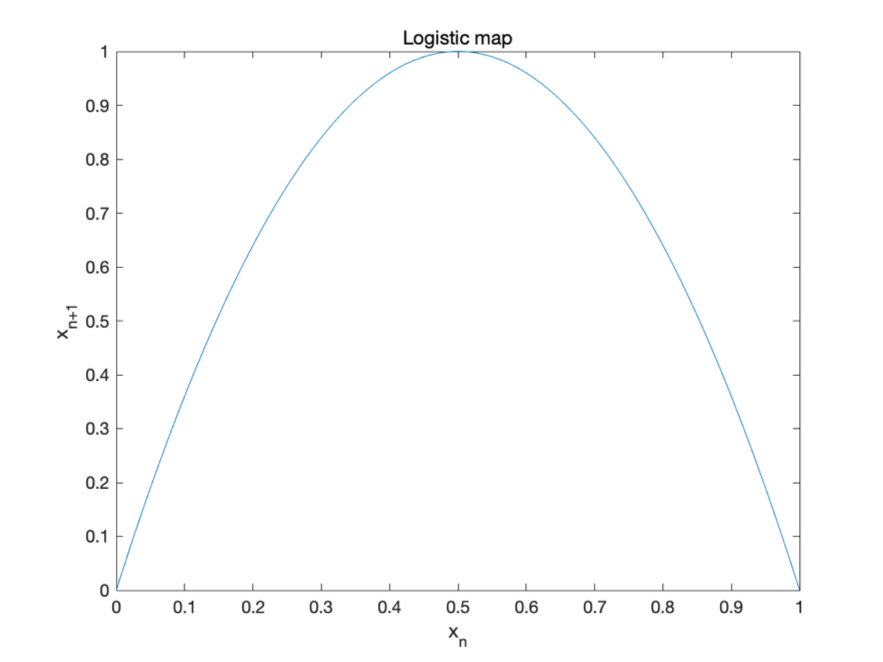
\includegraphics[scale=0.6]{logistic_phase.png}
    \caption{Logistic映射的相图($\gamma=4$)}
    \label{fig:logi_pha}
\end{figure}

Logistic映射的动力学过程可以看作是在一维相空间上的拉伸再折叠的过程。通过非线性动力学的知识\cite{strogatz2001nonlinear}可以得到,该系统在$\gamma$取不同值时表现出不同的动力学行为。当$0<\gamma<1$时,系统最终都会渐进的趋于0;当$1<\gamma<3$时,系统会收敛到一个不动点,该不动点的值为$x^*=(\gamma-1)/\gamma$,此时系统的极限行为会趋于该不动点的值;当$3<\gamma<3.57$时,系统的迭代会出现周期行为,随着$\gamma$的增大,周期的长度也会相应的增加,例如2周期,4周期,8周期轨道等,直到大约为$\gamma=3.57$时,周期的长度趋于无穷大;当$3.57<\gamma<4$时,系统的迭代会在周期类型和混沌类型之间来回切换,且大部分区域呈现混沌状态;直到$\gamma=4$时,系统处于完全混沌的状态。

Logistic映射的分岔图\cite{strogatz2001nonlinear}$x_n-\gamma$描述了系统随$\gamma$表现出的不同的动力学行为:
\begin{figure}[!]
	\centering
	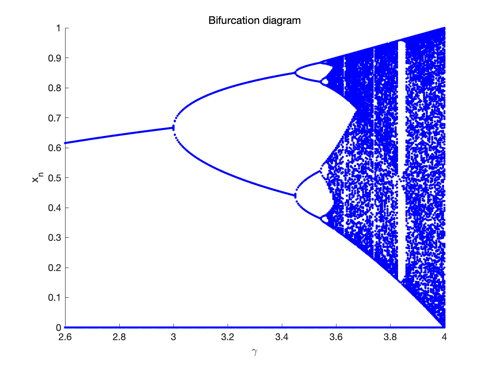
\includegraphics[scale=1]{logistic_bifurcation.png}
    \caption{Logistic映射的分岔图($2.6\leqslant\gamma\leqslant 4$)}
    \label{fig:logi_pha}
\end{figure}

李雅普诺夫指数是描述混沌现象的一个重要的指标,Logistic映射的李雅普诺夫指数图像$\lambda-\alpha$可通过式\ref{eq:lyapunov}计算,计算如下图所示:
\begin{figure}[!]
	\centering
	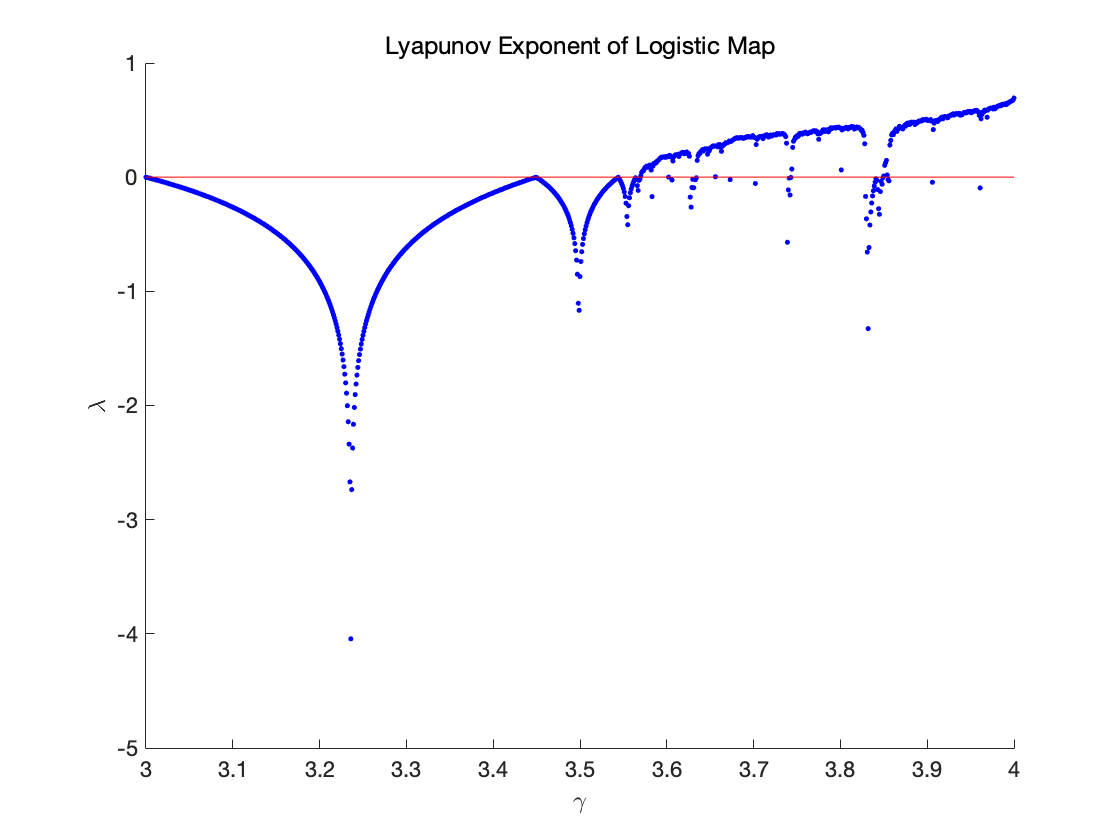
\includegraphics[scale=0.2]{logistic_lypn.png}
    \caption{Logistic映射的李雅普诺夫指数}
    \label{fig:logi_lypn}
\end{figure}
根据李雅普诺夫指数的性质\cite{strogatz2001nonlinear}:当$\lambda<0$时,映射系统收敛于某一不动点;当$\lambda=0$时,系统进行周期运动;当$\lambda>0$时,系统处于混沌状态。我们可以同样得到在$3.57<\gamma<4$区域,系统处于混沌状态(在$\gamma=3.83$处存在一三周期轨道),当$\gamma=4$时系统处于混沌状态。

不失一般性,在我们的Koopman分析中,我们取$\gamma=4$的一个特例,通过Logistic映射的动力学方程演化出一系列的数据,作为Koopman分析的源数据,以此来分析Logistic映射的系统特征。

\subsection{Logistic映射的Koopman算符本征函数}
在上一节的介绍中,我们探究了帐篷映射及其Koopman算符的本征函数。Logistic映射与帐篷映射有着非常相似的动力学特征,但其相图为非线性而非分段线性,非线性映射的一些性质会有所不同,且Logistic作为一个应用较广泛的混沌系统,其也有着丰富的研究价值。我们将探究Logistic映射Koopman算符的本征值与本征函数与动力学特征的关系及对相空间的划分,并将其与帐篷映射作一定的比较。

\subsubsection{正交完备基函数空间}

我们选取与帐篷映射相同的参数:演化格点数量$n=1000$,函数格点数量即基函数数量$m=4$,依此计算矩阵$U$的本征值与本征函数。图\ref{fig:logi_eig_RGFL}画出了$n=1000$,$m=4$时,四种不同的基函数(式\ref{fig:func_bas})下(矩形窗局函数、高斯基函数、傅里叶基函数、勒让德基函数)Logistic的本征函数,其中每个基函数下又包含4个不同的本征值对应的本征函数。

\begin{figure}[!]
    \centering
    \subfloat[矩形窗基函数]{
      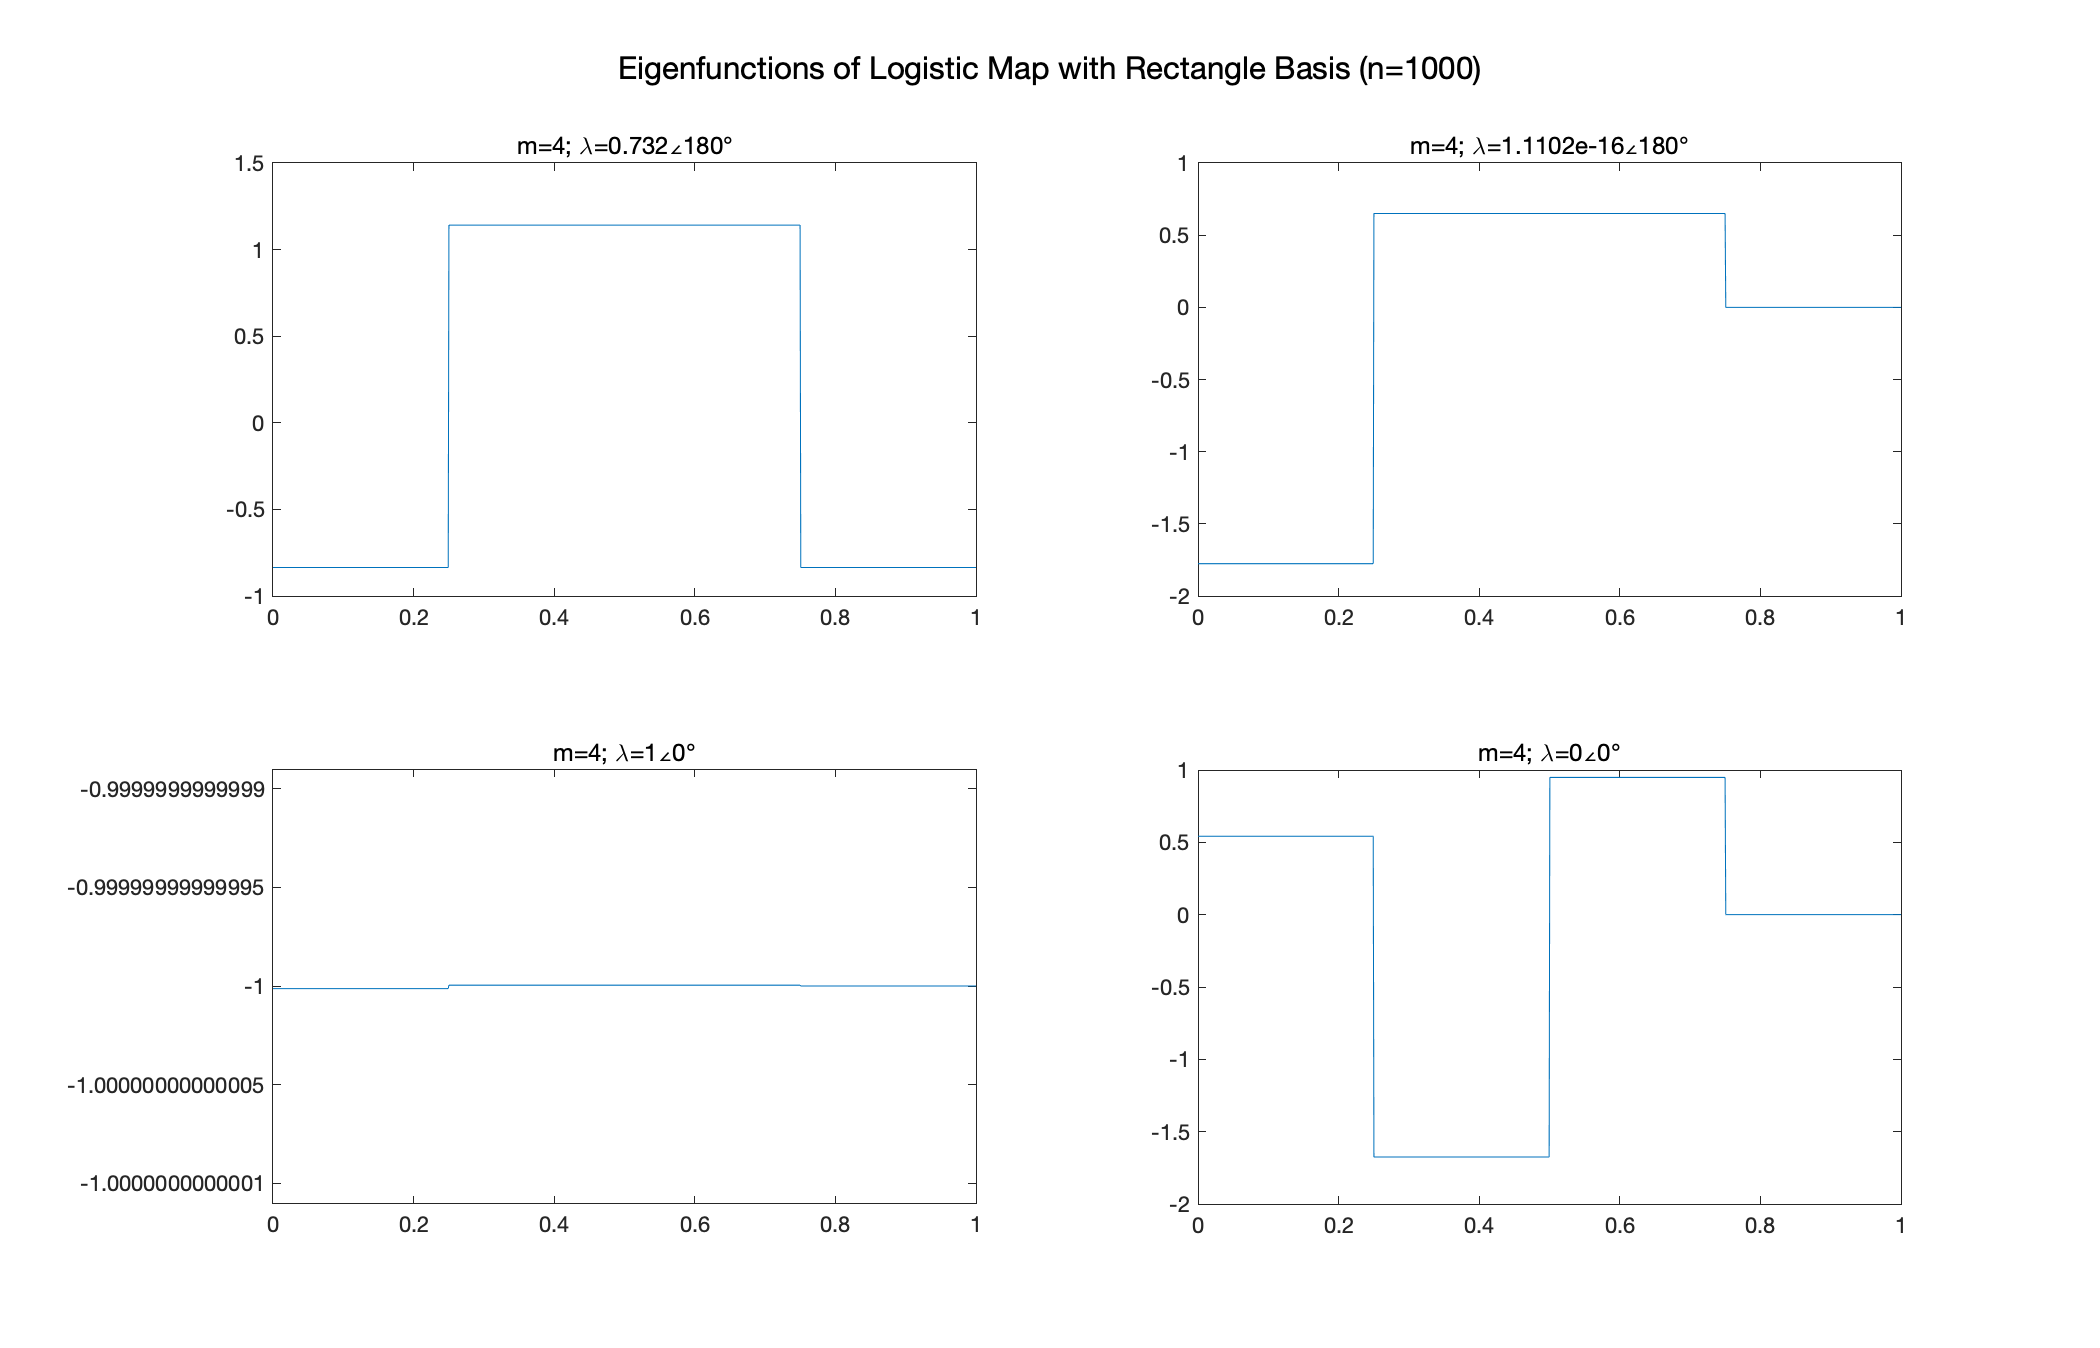
\includegraphics[scale=0.2]{logistic/Logistic_eigen_Rectangle_n1000_m4}}
    \subfloat[高斯基函数]{
      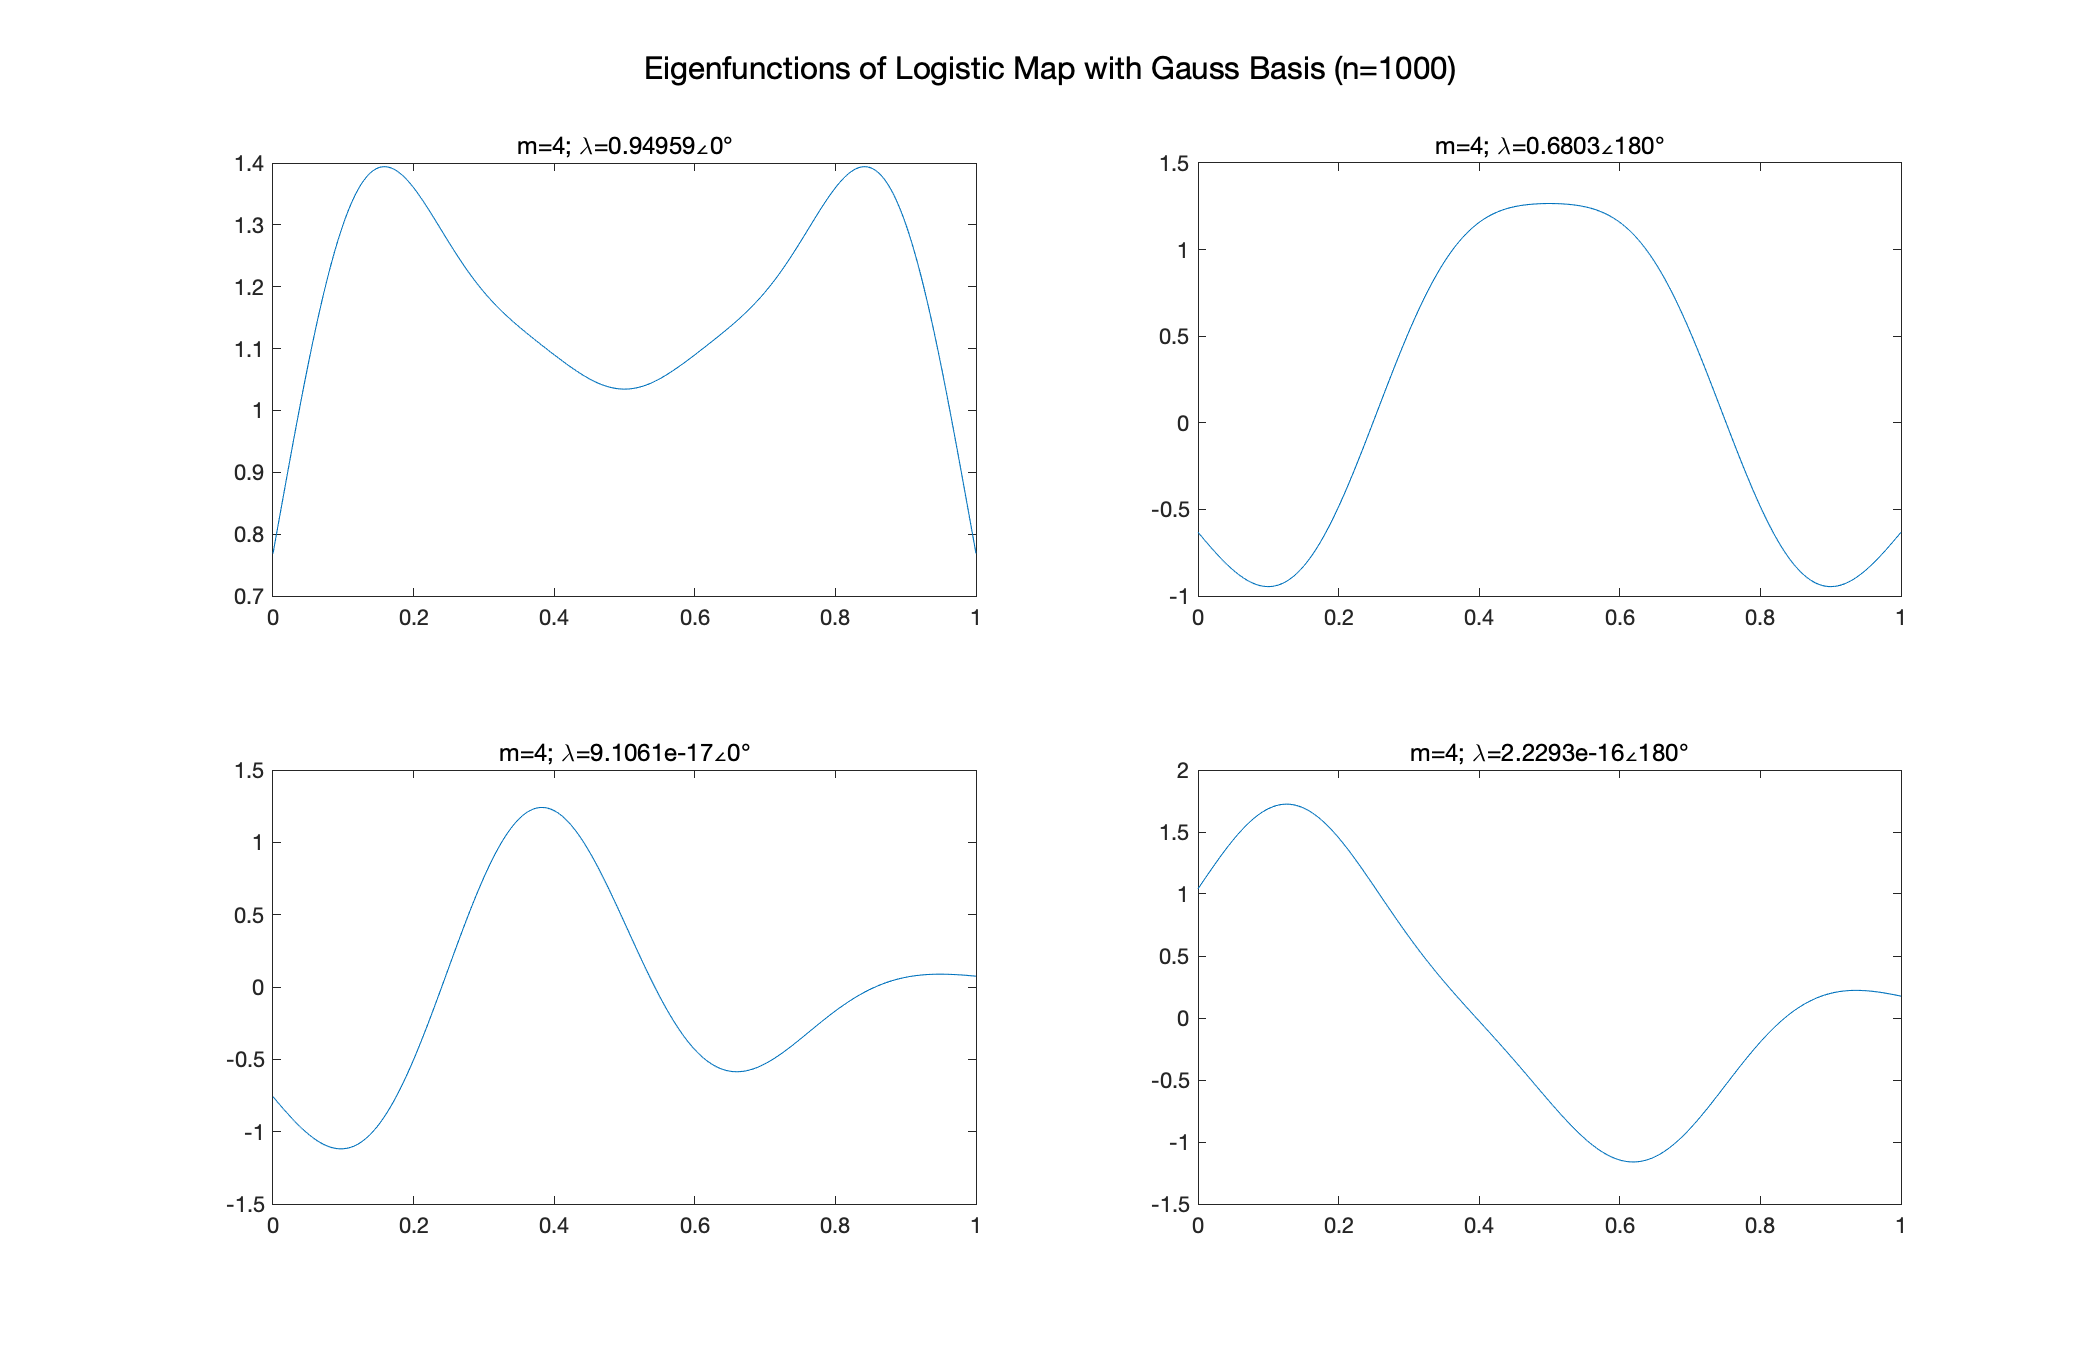
\includegraphics[scale=0.2]{logistic/Logistic_eigen_Gauss_n1000_m4}}
      \\
    \subfloat[傅里叶基函数]{
      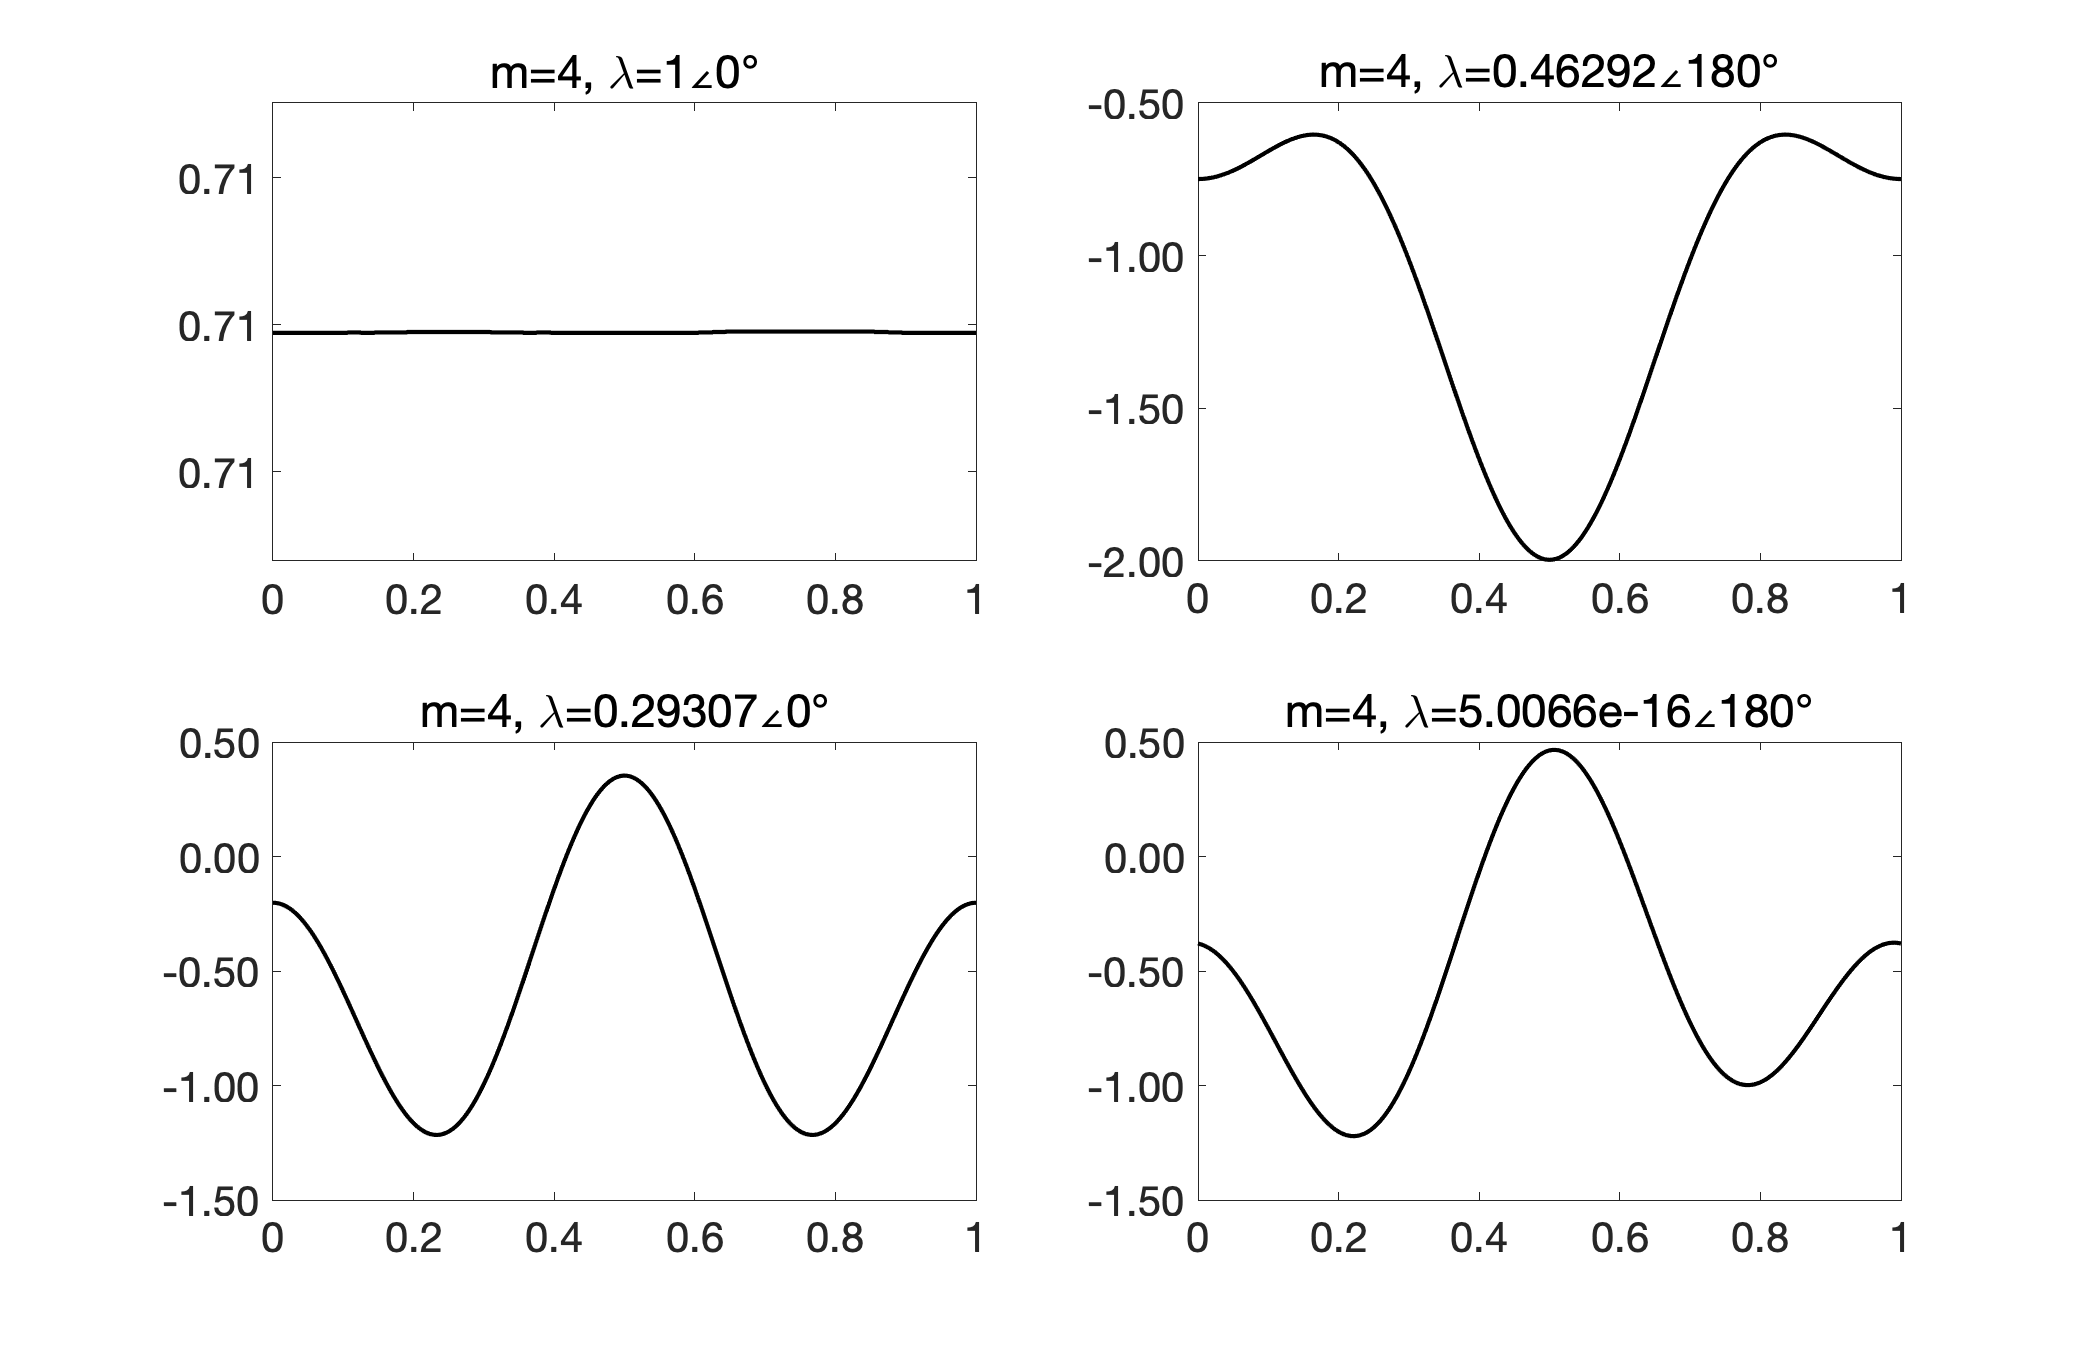
\includegraphics[scale=0.2]{logistic/Logistic_eigen_Fourier_n1000_m4}}
    \subfloat[勒让德基函数]{
      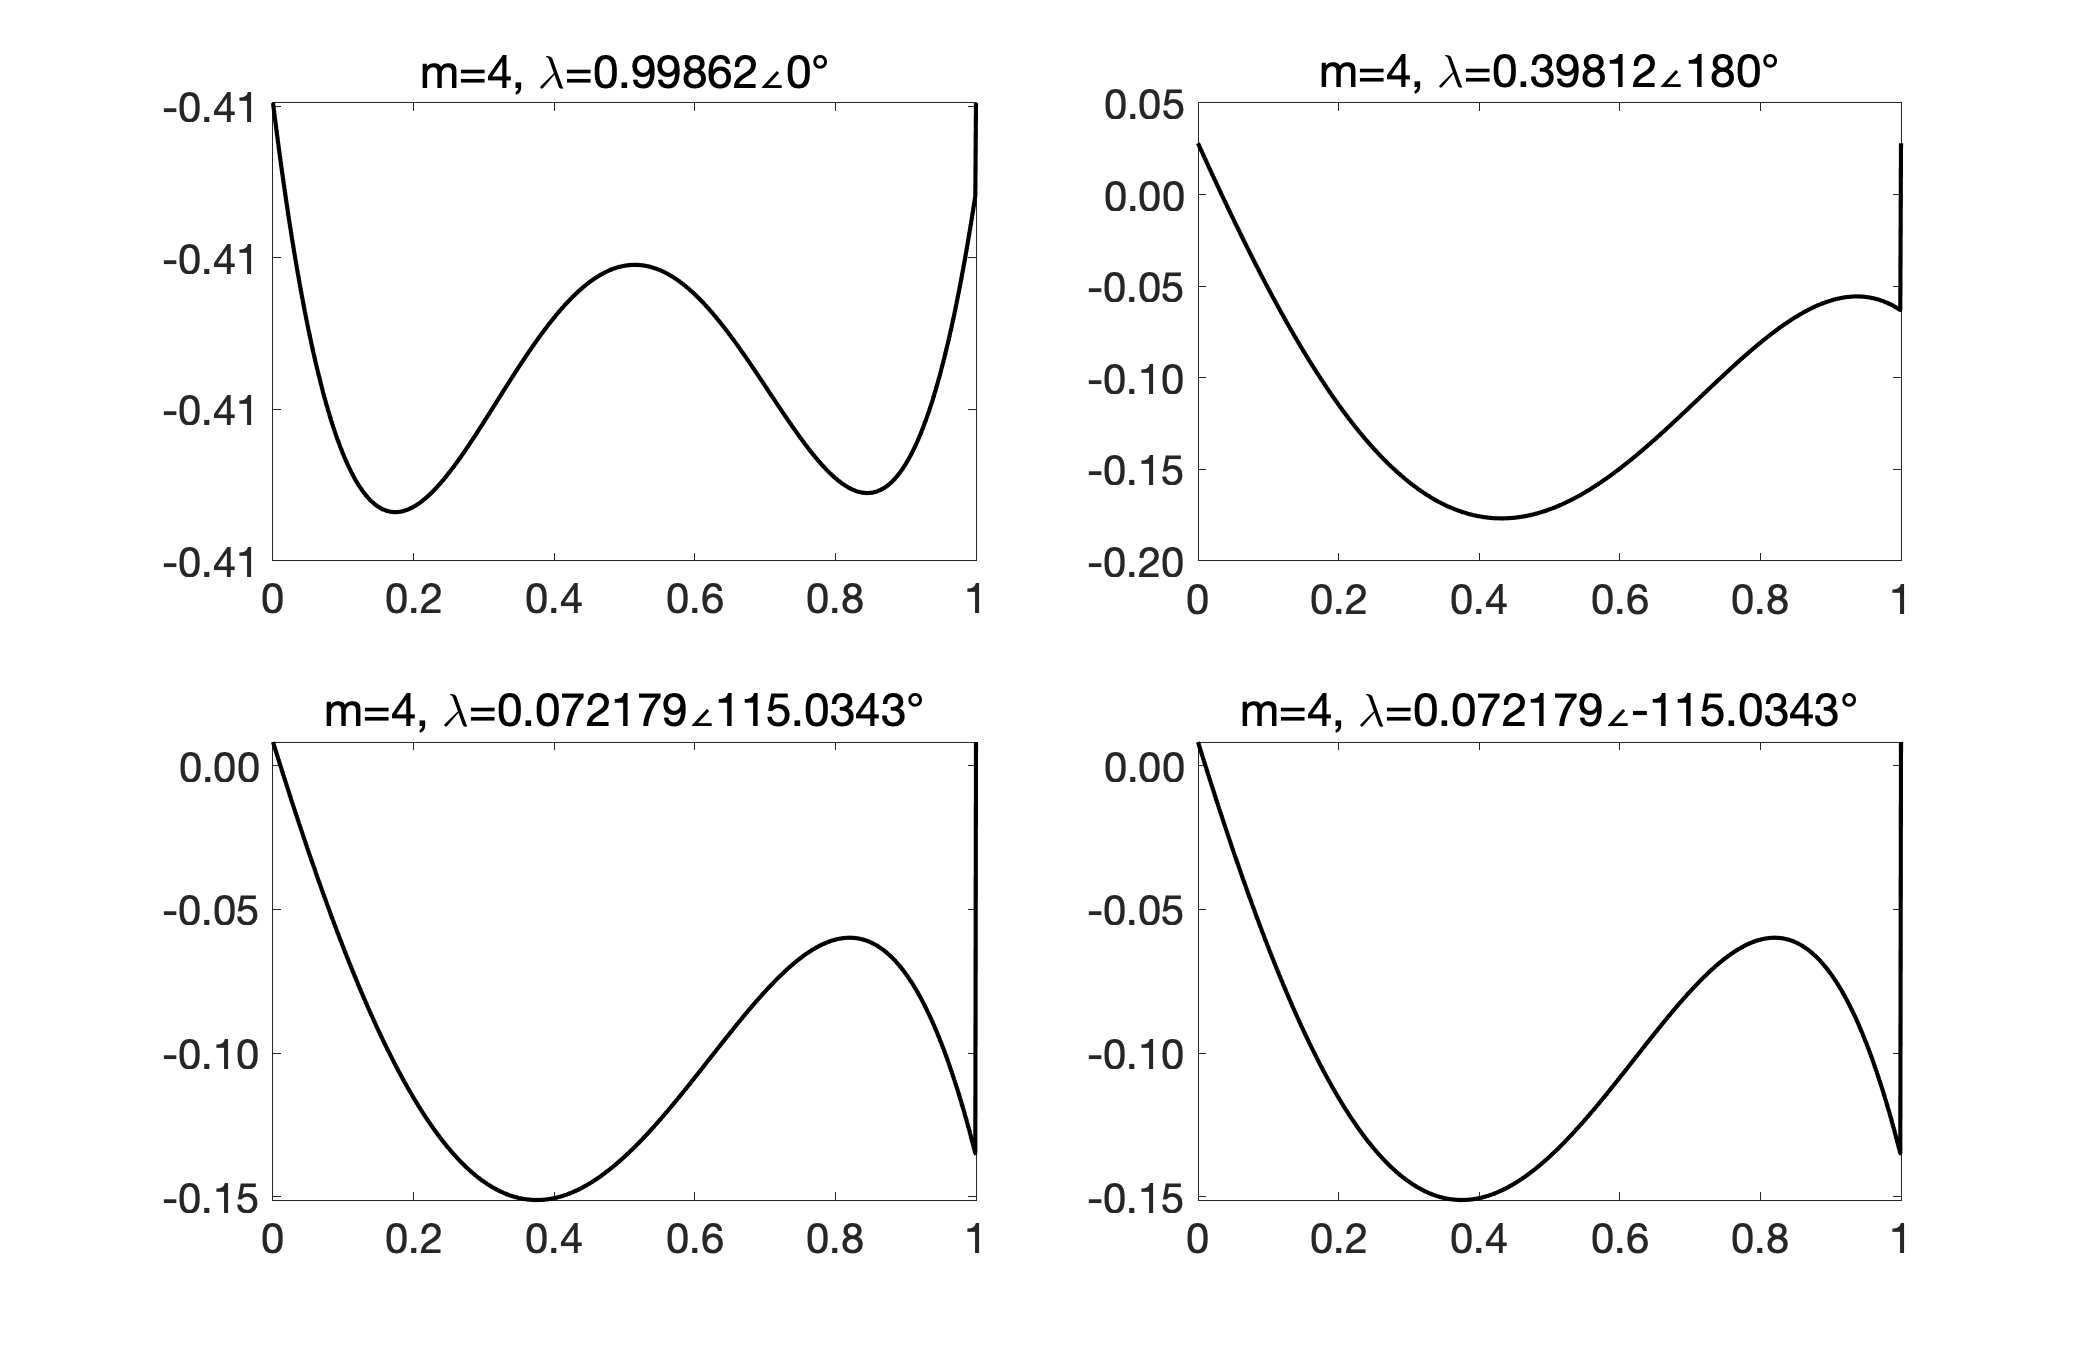
\includegraphics[scale=0.2]{logistic/Logistic_eigen_Legendre_n1000_m4}}
    \caption{四种基函数下Logistic映射的本征函数($m=4$)}\label{fig:logi_eig_RGFL}
\end{figure}

我们可以在四种基函数下Logistic映射的本征函数(图\ref{fig:logi_eig_RGFL})中得到与帐篷映射类似的结论:在不同的基函数下,Koopman算符的本征函数表现出极大的差异;本征函数总是在选取的基函数空间内,即从数学上每个本征函数都由所有的基函数线性组合而成;局部函数能通过每个基函数比例系数的大小来体现对相空间的划分,因此我们更关心这种局部函数;我们不可能选取一个完全完备的函数空间,我们的本征函数只是在此函数空间的一个近似。函数空间的维度更高,可以描述的本征函数的维度也就越高,则对于局部函数如高斯函数而言,我们描述本征函数的精细度就更高。我们取四种基函数及基函数数量$m=2,3,4,8,10,16,20,50,100$时对应的本征值与本征函数,以此来反映出随着函数空间的精细度的提高本征函数的变化。

\begin{figure}[!]
  \centering
  \subfloat[矩形窗基函数]{
    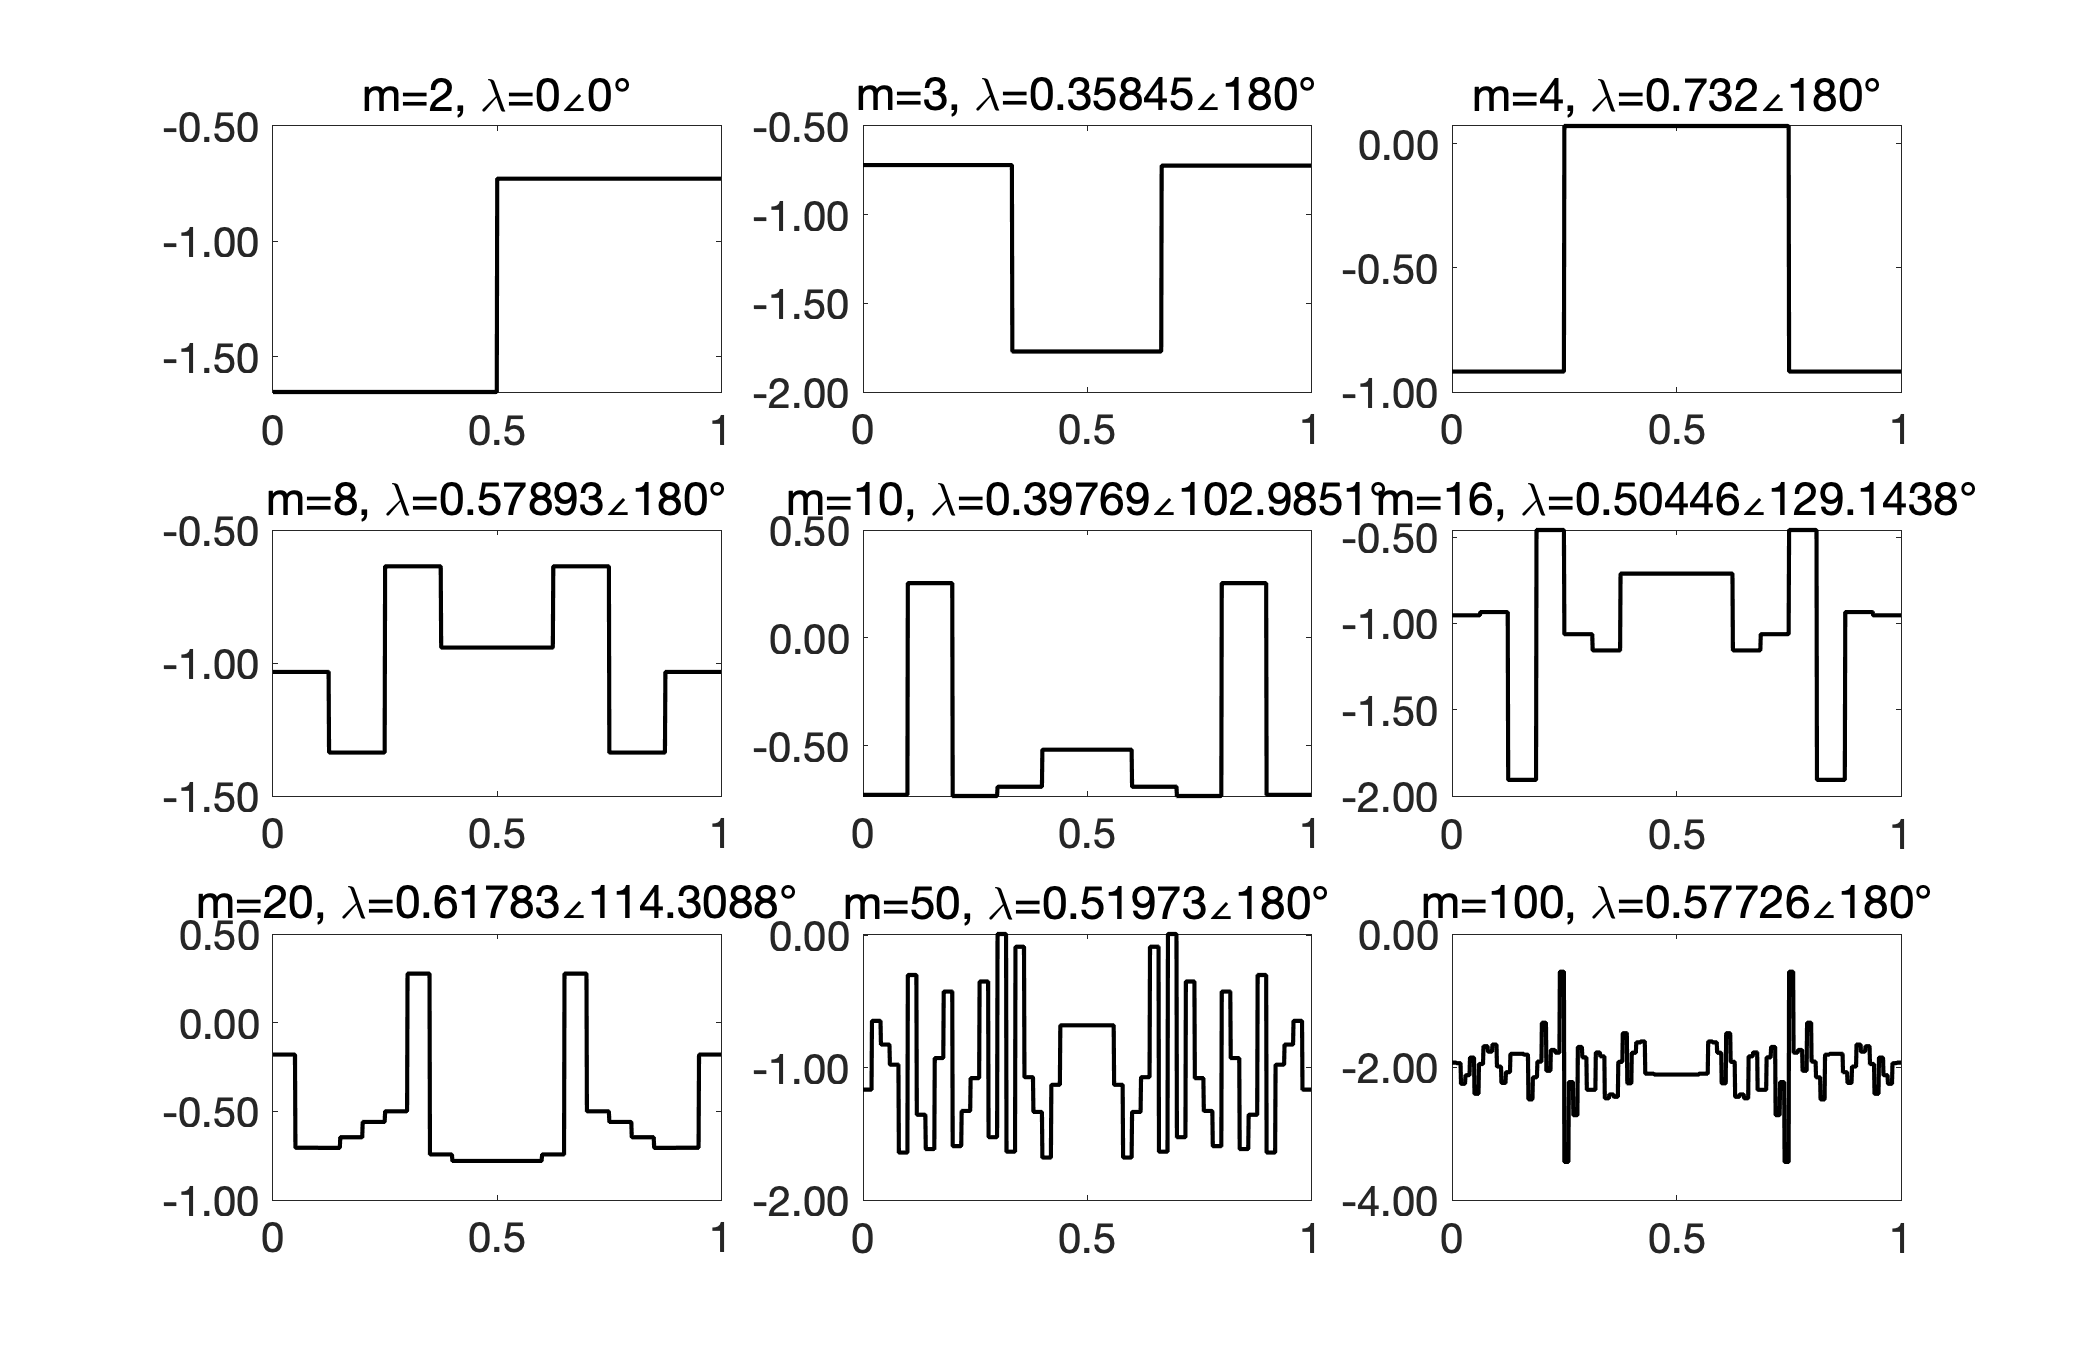
\includegraphics[scale=0.2]{logistic/Logistic_eigen_Rectangle_n1000_m2-3-4-8-10-16-20-50-100}}
  \subfloat[高斯基函数]{
    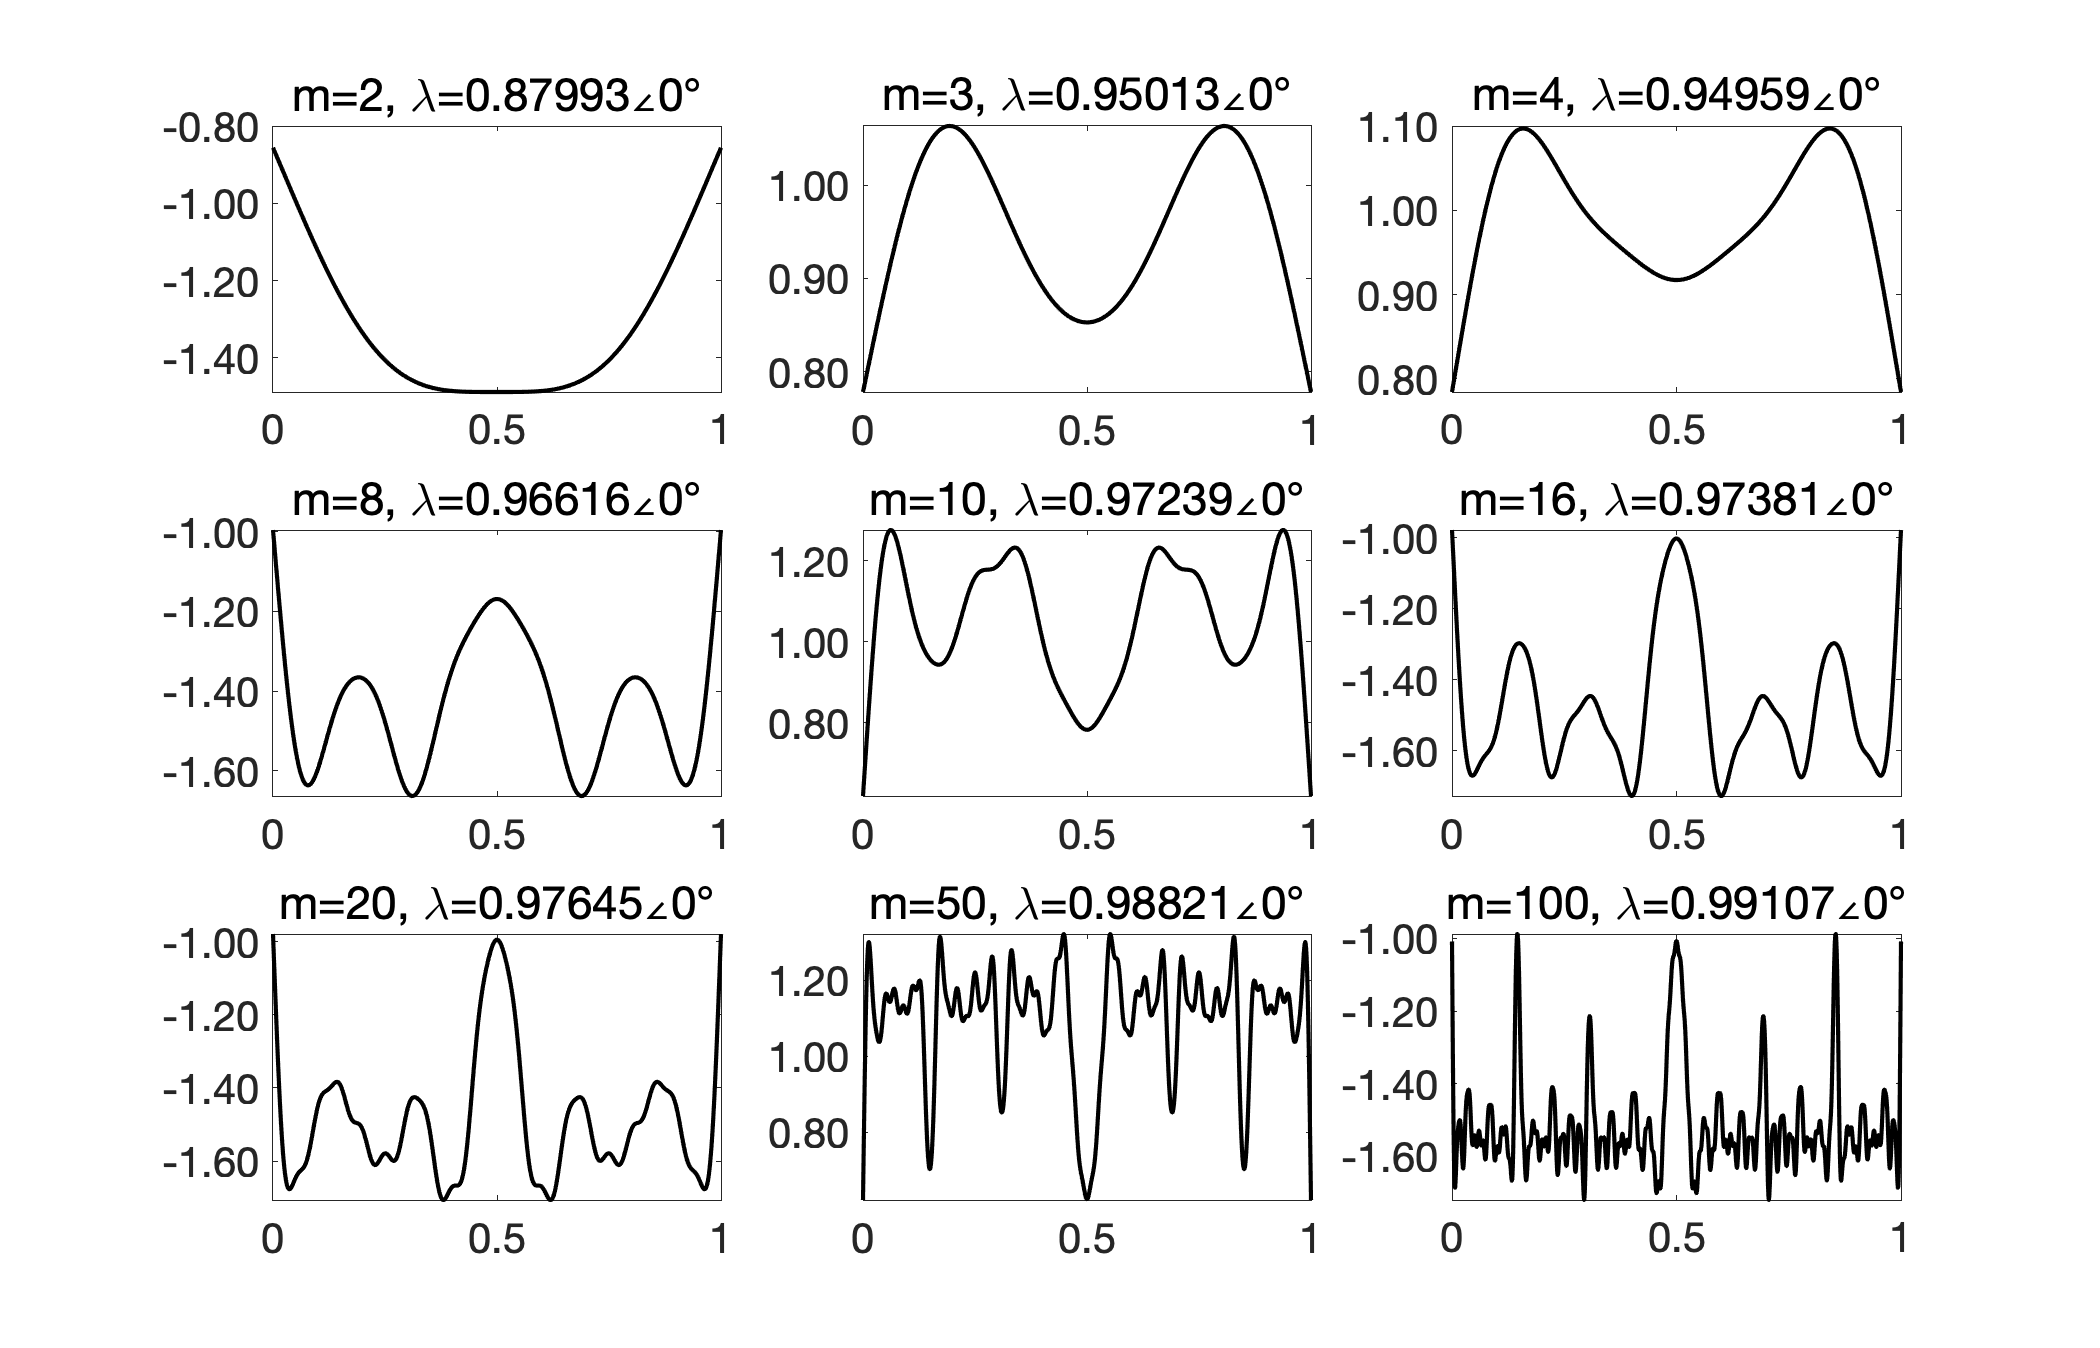
\includegraphics[scale=0.2]{logistic/Logistic_eigen_Gauss_n1000_m2-3-4-8-10-16-20-50-100}}
    \\
  \subfloat[傅里叶基函数]{
    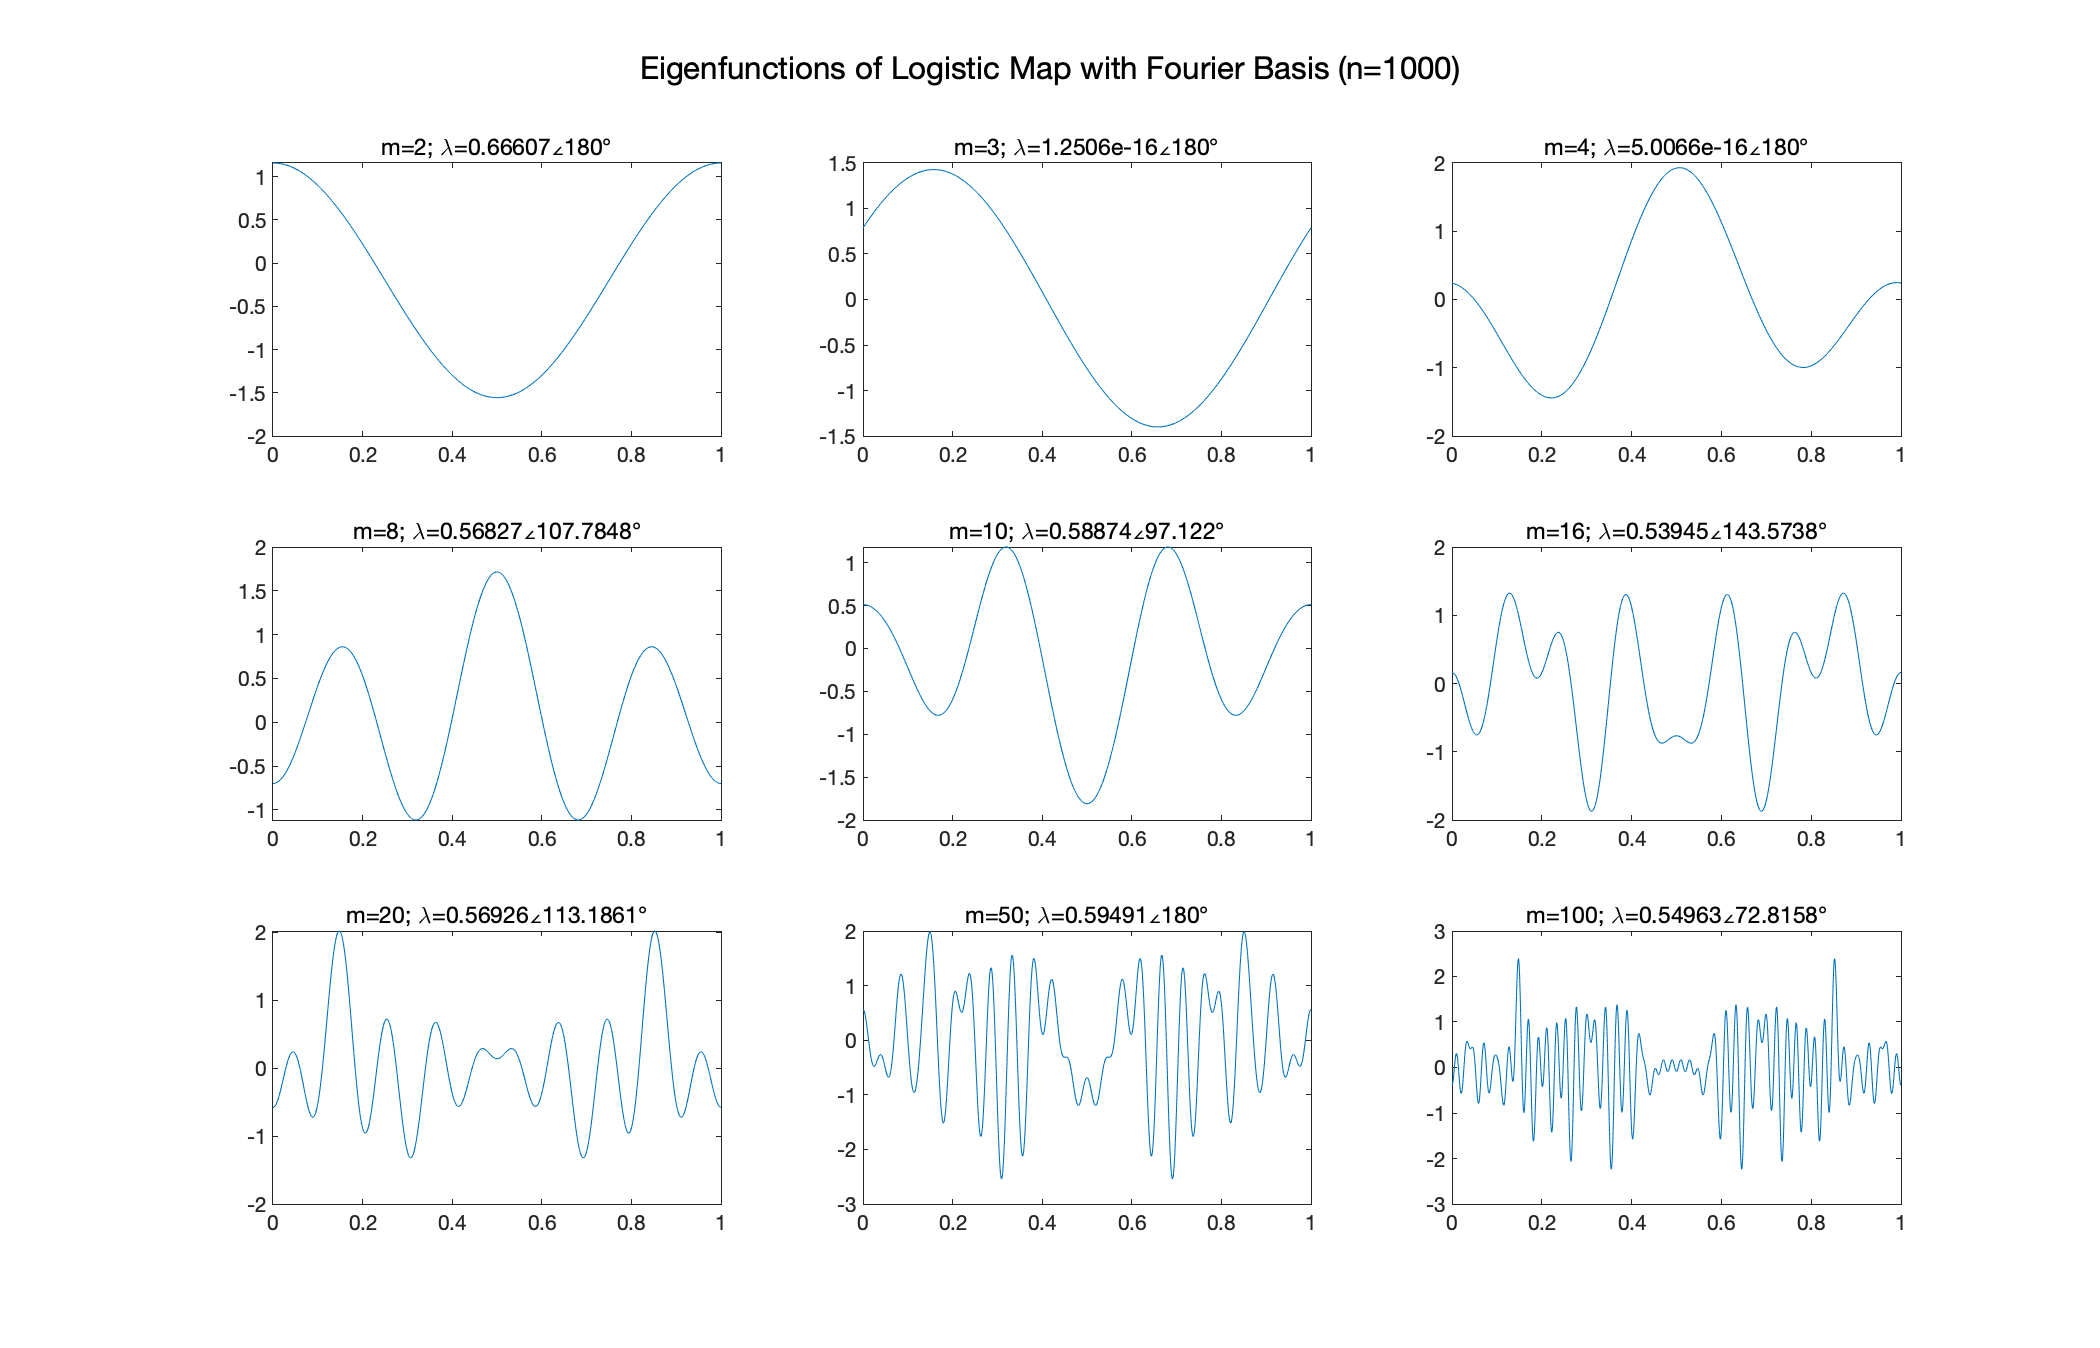
\includegraphics[scale=0.2]{logistic/Logistic_eigen_Fourier_n1000_m2-3-4-8-10-16-20-50-100}}
  \subfloat[勒让德基函数]{
    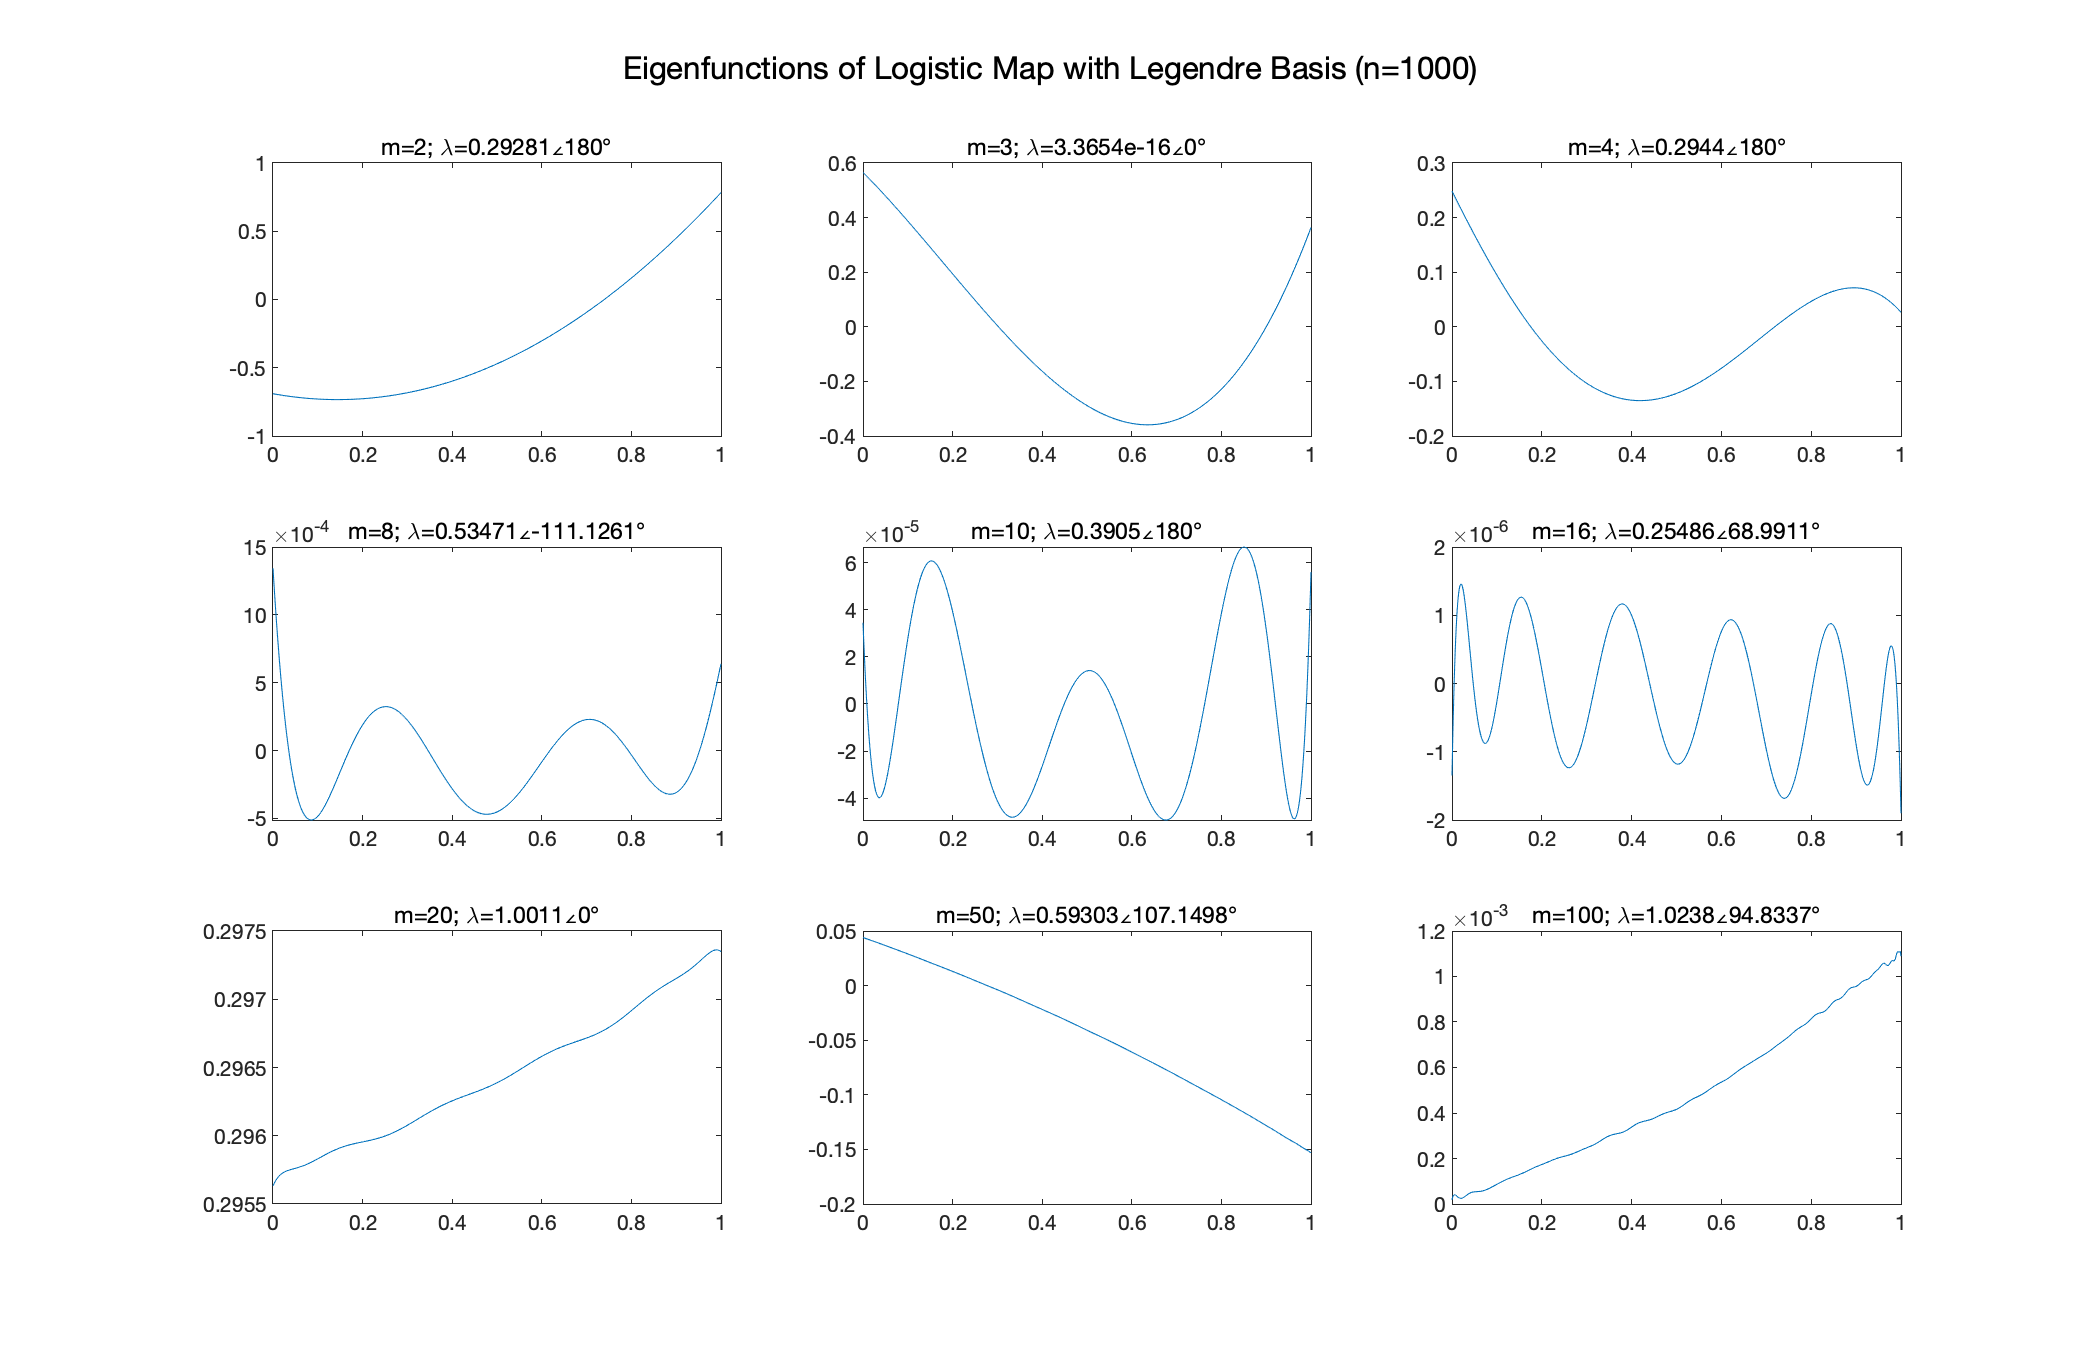
\includegraphics[scale=0.2]{logistic/Logistic_eigen_Legendre_n1000_m2-3-4-8-10-16-20-50-100}}
  \caption{不同基函数数量下Logistic映射的本征函数}\label{fig:logi_eig_RGFL_multim}
\end{figure}

在图\ref{fig:logi_eig_RGFL_multim}中,我们同样发现,当基函数数量增加时,本征函数图像的频率增加了,即描述本征函数的精细度增加了。且本征函数的变化有一定的规律:随着基函数数量的增加而使得描述本征函数的精细度的增加。在Logistic映射中,$x=\frac{1}{2}$将相空间$(0,1)$分为对称的两部分,而每部分中又有极值点将每个部分各自分为两部分,这与帐篷映射的性质较为相似,但是由于Logistic为非线性映射,其再次进行划分的边界则与帐篷映射有所区别。

\subsubsection{自然基函数空间}
在式\eqref{eq:Koop_kl2}中,我们通过构造自然基函数格点得到了Koopman算符的矩阵表示,选取合适的参数:演化格点$n=1000$,基函数数量$m=4$下,我们可以计算得到4个Koopman算符$U$的本征值与本征函数并将其画到相空间中,如图\ref{fig:Logistic_eigen_natural_n1000_m4}。我们可以发现在自然基函数空间下,本征函数的图像变得更为尖锐,但也更接近Logistic映射的相图。
\begin{figure}[!]
	\centering
	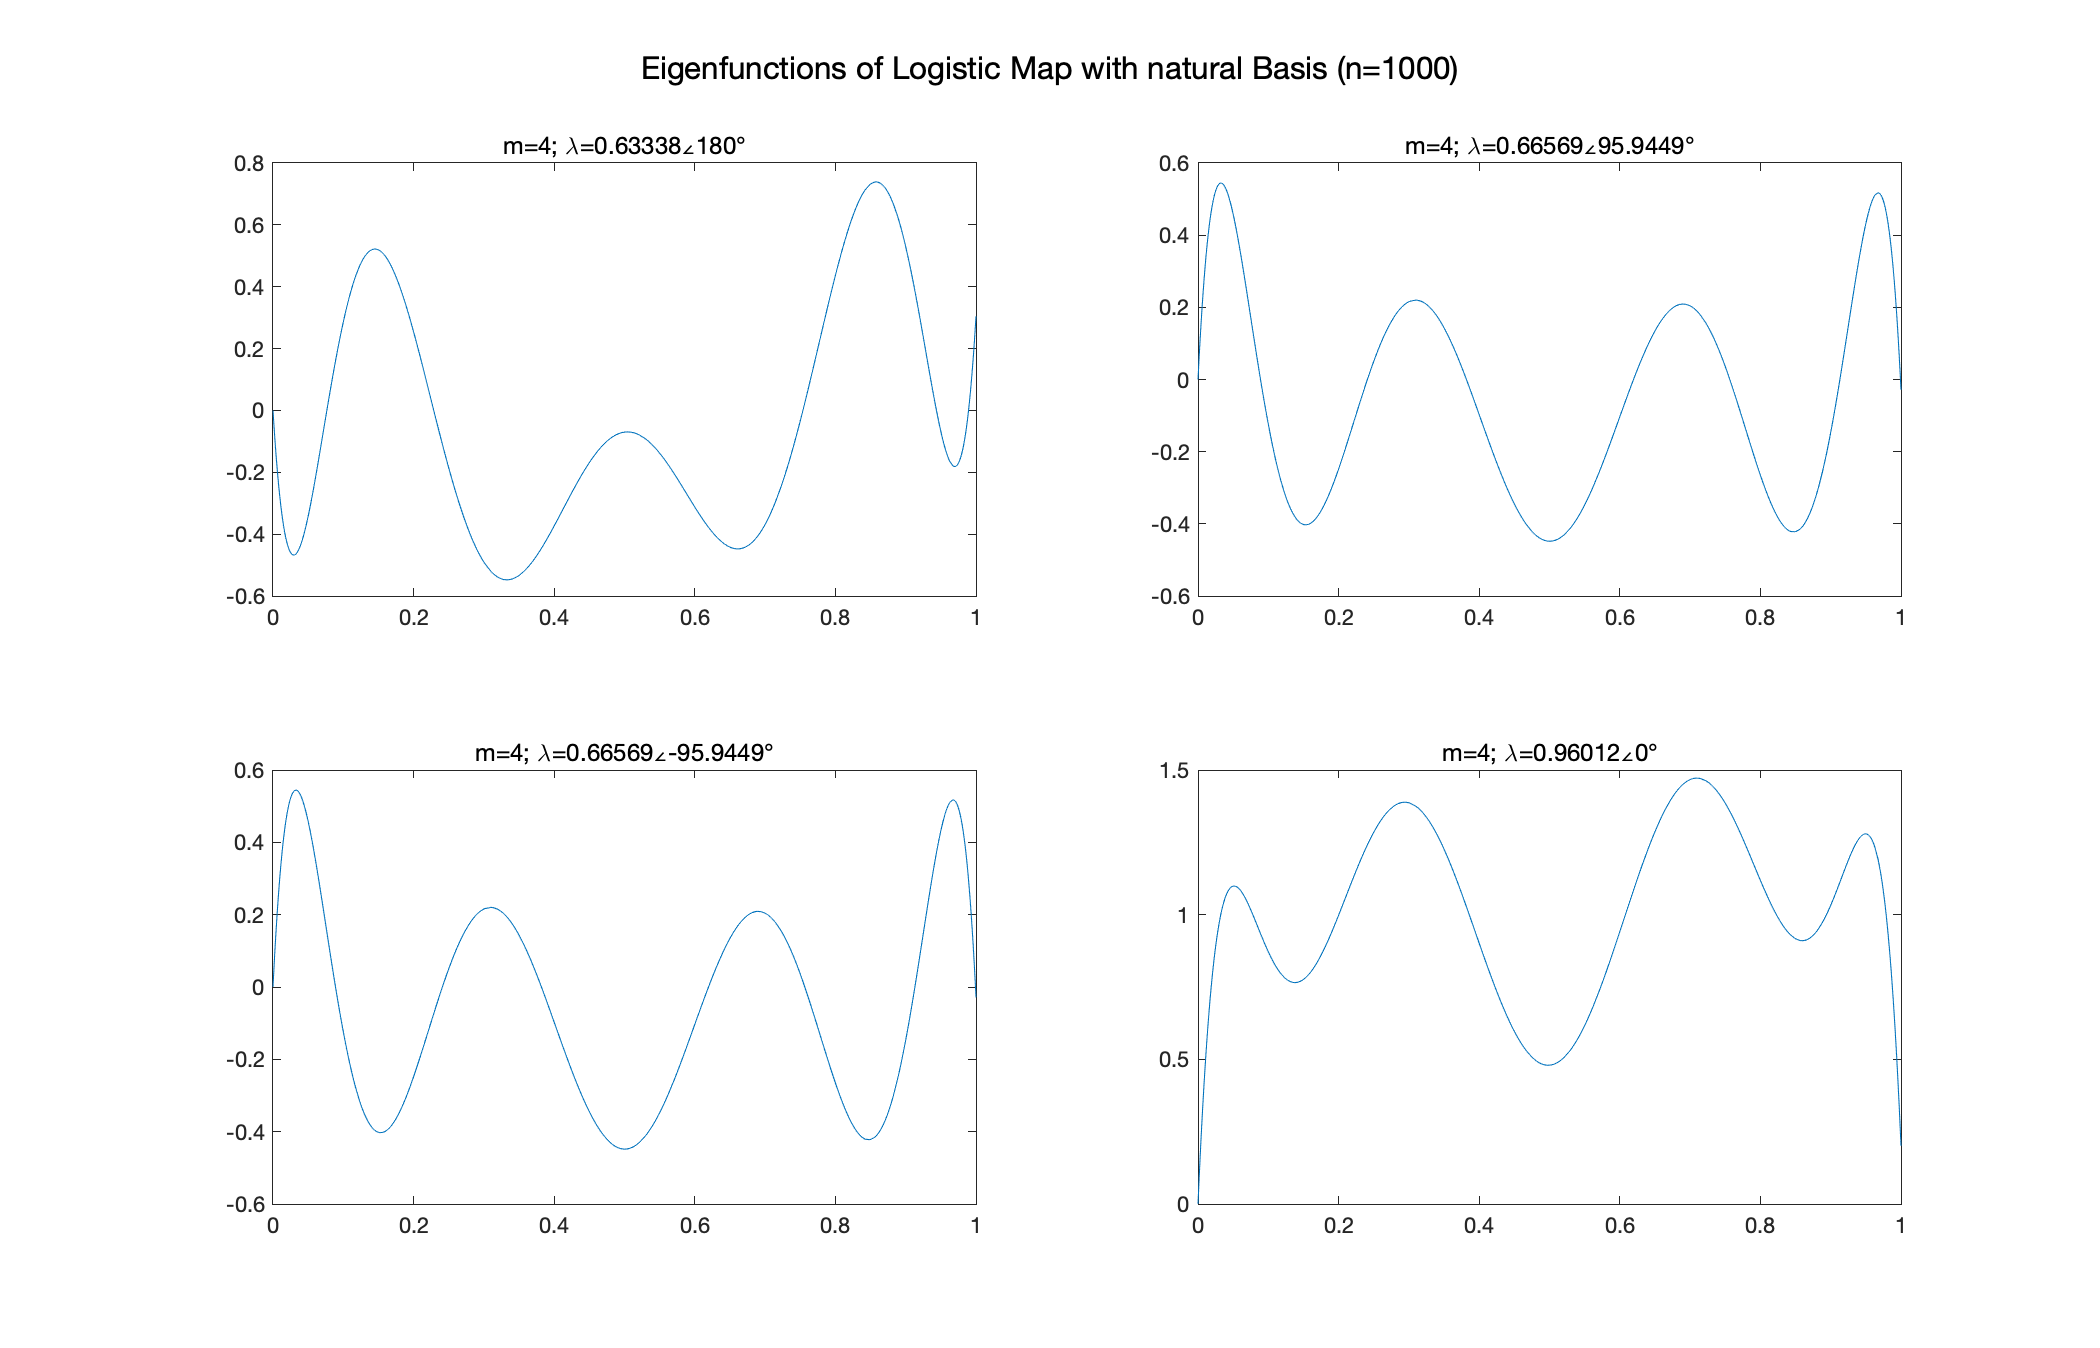
\includegraphics[scale=0.4]{logistic/Logistic_eigen_natural_n1000_m4}
    \caption{自然基函数下Logistic映射的本征函数($m=4$)}\label{fig:Logistic_eigen_natural_n1000_m4}
\end{figure}
当我们取不同的基函数数量$m=1,2,3,4,5,6,7,8,9$且取$\lambda\approx 1$的本征函数,我们可以得到图\ref{Logistic_eigen_natural_n5000_m1-2-3-4-5-6-7-8-9}。从图中我们可以发现,基函数数量每增加1,极值点出现的个数近似增加两倍。而我们又考虑到Logistic映射$T$及其多次映射$T^n$的关系:映射次数$n$每增加一次,$T^n$的相图变多增加一次弯折,即极值点的数量增加一倍。这与我们看到的本征函数图像的极值点较为相似。
\begin{figure}[!]
	\centering
	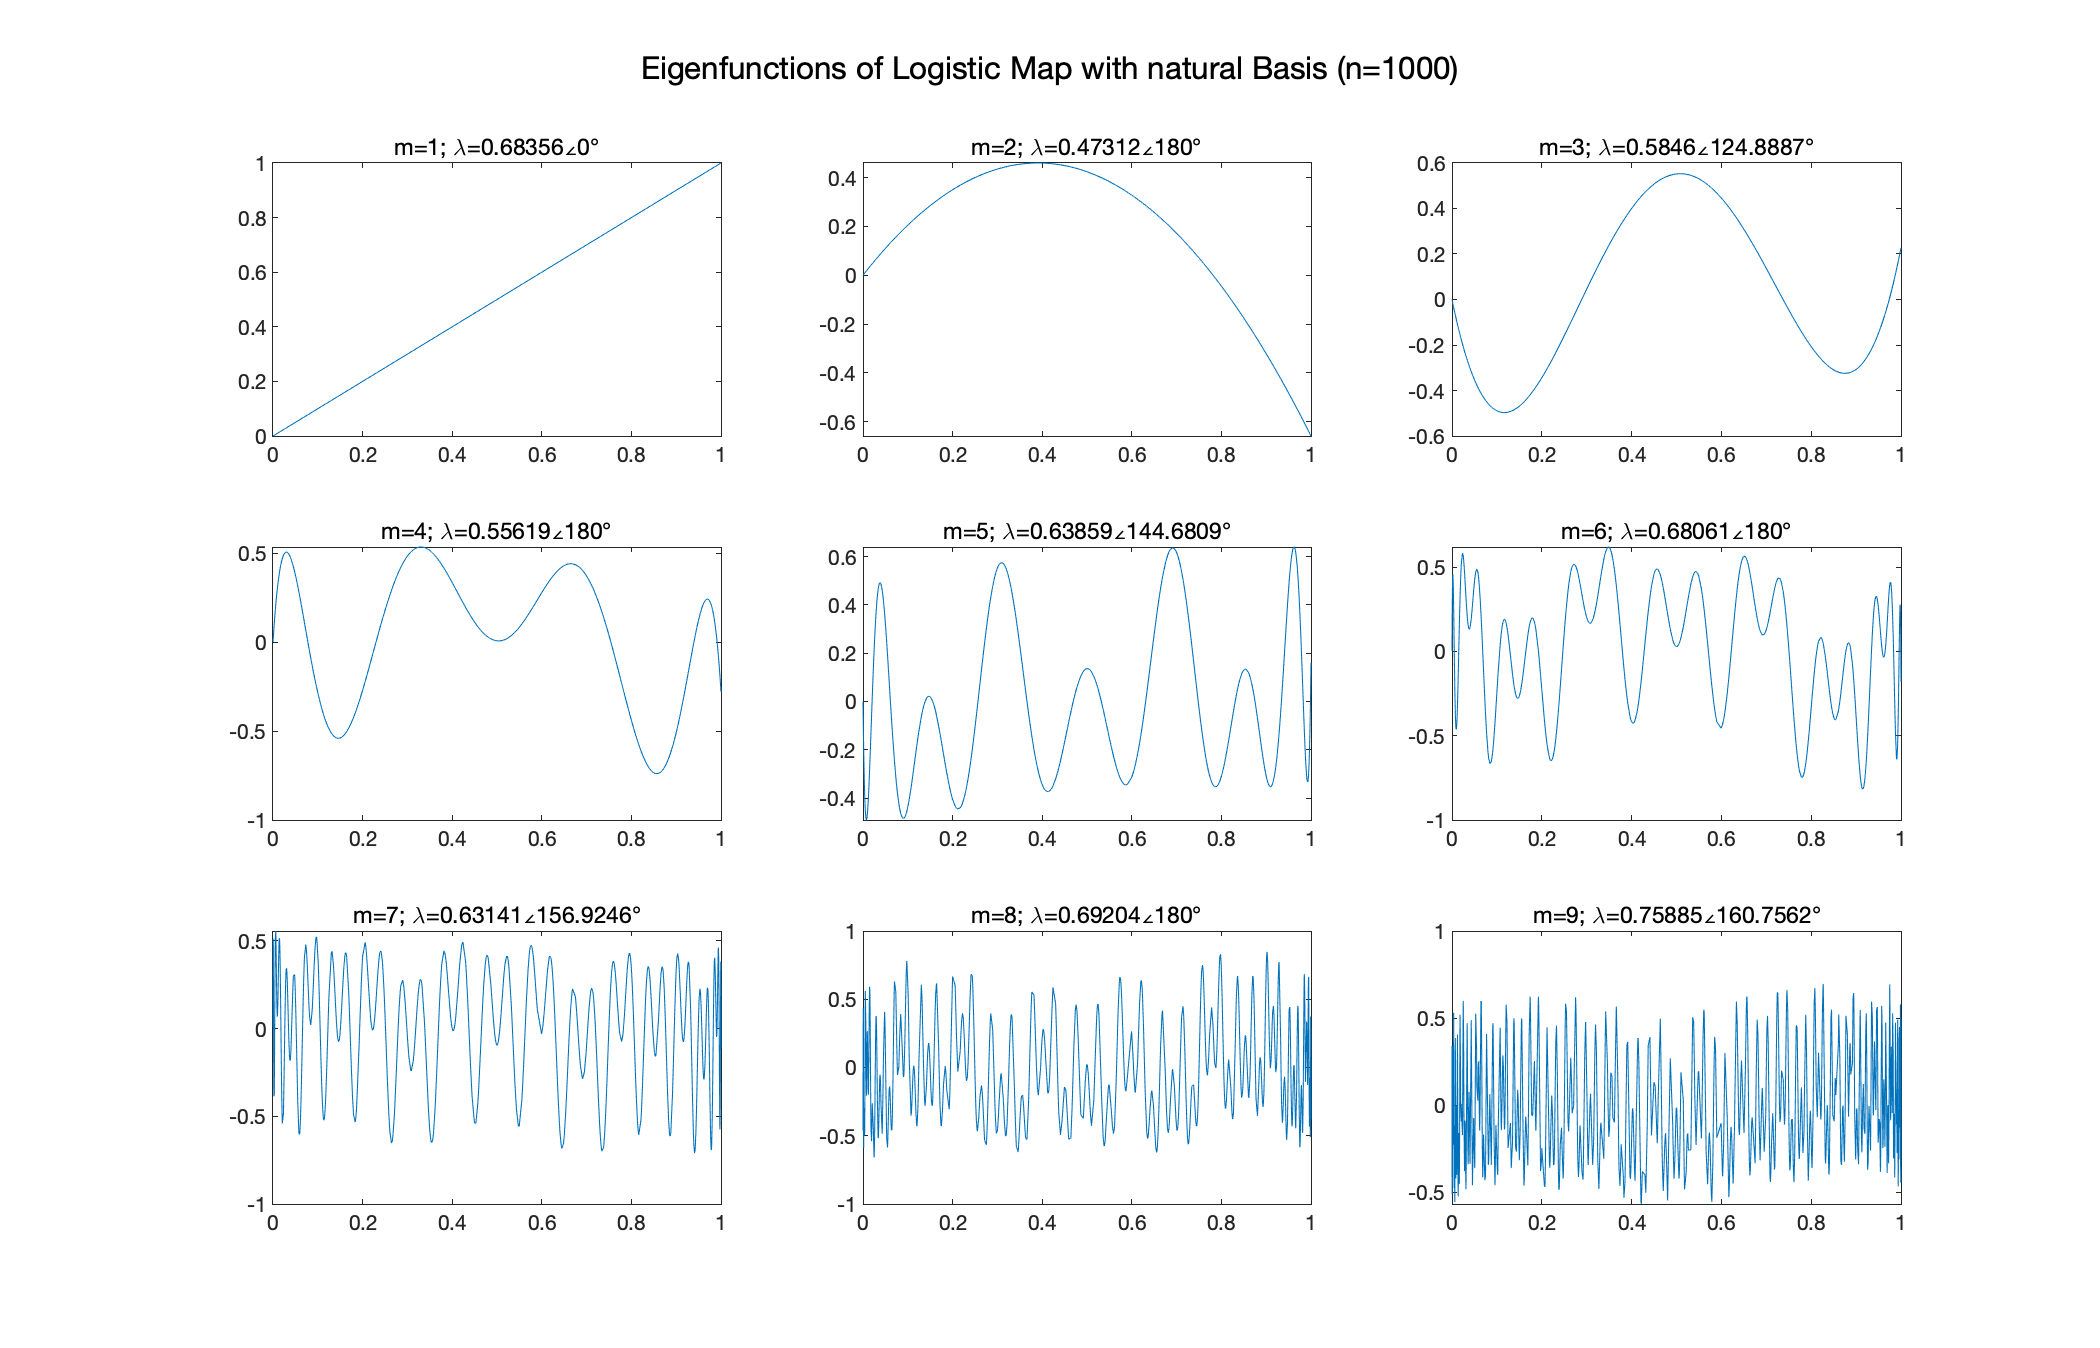
\includegraphics[scale=0.4]{logistic/Logistic_eigen_natural_n1000_m1-2-3-4-5-6-7-8-9}
    \caption{不同基函数数量下Logistic映射的本征函数}\label{Logistic_eigen_natural_n5000_m1-2-3-4-5-6-7-8-9}
\end{figure}
无论是在正交完备基函数族还是在自然基函数中,我们都发现了在本征函数中的一些特殊的极值点,在帐篷映射在我们已经得到了结论:我们可以通过Koopman算符确定动力学系统的边界点,且可以通过增加函数格点数量来精确的寻找重要的边界点,而其他层次的边界点也可以通过迭代关系来确定。在Logistic映射中我们也有充分的理由相信其满足同样类似的规律。

\subsection{Koopman算符对Logistic映射的相空间划分}
Logistic映射存在两个不动点$x=\frac{1}{2}$和$x=\frac{3}{4}$,类似于帐篷映射,我们可以得到Logistic映射一系列的边界点。不动点$x=0$的一系列原像点如表\ref{tab:logi_bound0}所示。将其按照\textbf{层次}(经过多少次演化才达到不动点)作出图像,如图\ref{fig:logi_bound0}。

\begin{table}[]
    \centering
    \begin{tabular}{|c|c|}
    \hline
    迭代次数 & 边界点($x=0$) \\ \hline
    1 & 0,\textbf{\underline{1}} \\ \hline
    2 & 0,\textbf{\underline{0.5}},1 \\ \hline
    3 & 0,\textbf{\underline{0.1464}},0.5,\textbf{\underline{0.8536}},1 \\ \hline
    4 & 0,\textbf{\underline{0.0381}},0.1464,\textbf{\underline{0.3087}},0.5,\textbf{\underline{0.6913}},0.8536,\textbf{\underline{0.9619}},1 \\ \hline
    5 & \begin{tabular}[c]{@{}l@{}}0,\textbf{\underline{0.0096}},0.0381,\textbf{\underline{0.0843}},0.1464,\textbf{\underline{0.2222}},0.3087,\textbf{\underline{0.4024}},\\ 0.5,\textbf{\underline{0.5975}},0.6913,\textbf{\underline{0.7778}},0.8536,\textbf{\underline{0.9157}},0.9619,\textbf{\underline{0.9904}},1\end{tabular} \\ \hline
    \end{tabular}
    \caption[Logistic映射的边界点($x=0$)]{Logistic映射的边界点($x=0$):经过多少次迭代可以到达不动点$x=\frac{3}{4}$,下划线的点是每层次的新增点}\label{tab:logi_bound0}
\end{table}

\begin{figure}[!]
	\centering
	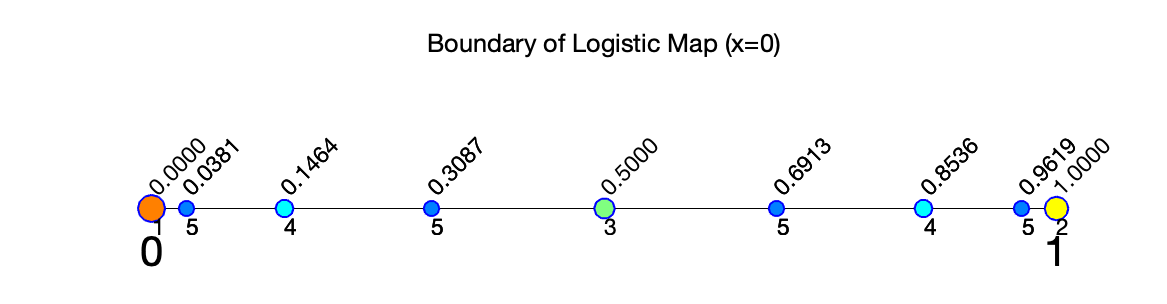
\includegraphics[scale=0.6]{logistic/Logistic_boundarys_x0}
    \caption[Logistic映射的边界点($x=0$)]{Logistic映射的边界点($x=0$):相同大小和颜色的点同属于一个层次}\label{fig:logi_bound0}
\end{figure}
同样,对于另一个不动点$x=\frac{3}{4}$,我们同样作出其一系列原像点(表\ref{tab:logi_bound3-4}),且按层次绘制其在相空间的位置(图\ref{fig:logi_bound3-4})。
\begin{table}[]
    \centering
    \begin{tabular}{|c|c|}
    \hline
    迭代次数 & 边界点($x=\frac{3}{4}$) \\ \hline
    0 & 0.75 \\ \hline
    1 & \textbf{\underline{0.25}},0.75 \\ \hline
    2 & \textbf{\underline{0.0670}},0.25,0.75,\textbf{\underline{0.9330}} \\ \hline
    3 & \textbf{\underline{0.0170}},0.0670,0.25,\textbf{\underline{0.3706}},\textbf{\underline{0.6294}},0.75,0.9330,\textbf{\underline{0.9830}} \\ \hline
    4 & \begin{tabular}[c]{@{}l@{}}\textbf{\underline{0.0043}},0.0170,0.0670,\textbf{\underline{0.1033}},\textbf{\underline{0.1956}},0.25,0.3706,\textbf{\underline{0.4347}},\\ \textbf{\underline{0.5653}},0.6294,0.75,\textbf{\underline{0.8044}},\textbf{\underline{0.8967}},0.9330,0.9830,\textbf{\underline{0.9957}}\end{tabular} \\ \hline
    \end{tabular}
    \caption[Logistic映射的边界点($x=\frac{3}{4}$)]{Logistic映射的边界点($x=\frac{3}{4}$):经过多少次迭代可以到达不动点$x=\frac{3}{4}$,下划线的点是每层次的新增点}\label{tab:logi_bound3-4}
\end{table}

\begin{figure}[!]
	\centering
	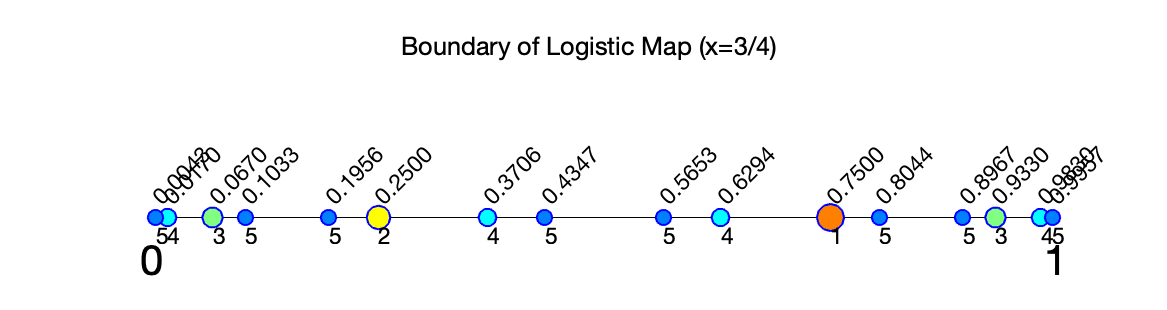
\includegraphics[scale=0.6]{logistic/Logistic_boundarys_x3-4}
    \caption[Logistic映射的边界点]{Logistic映射的边界点($x=\frac{3}{4}$):相同大小和颜色的点同属于一个层次}\label{fig:logi_bound3-4}
\end{figure}

类比帐篷映射,我们将本征函数和边界点的位置进行对比观察:在图\ref{fig:Logistic_eigen_noise_n1000m2d0}中,我们取不同的基函数数量$m=2,3,4,5,8,10,15,20$,并绘制最多9个本征函数图像,将本征函数图像的极值点标出,并将Logistic的边界点同时标出,以此来对比二者之间的关系。

\begin{figure}[!]
    \centering%[2,3,4,5,8,10,15,20]
    \subfloat[m=2]{
      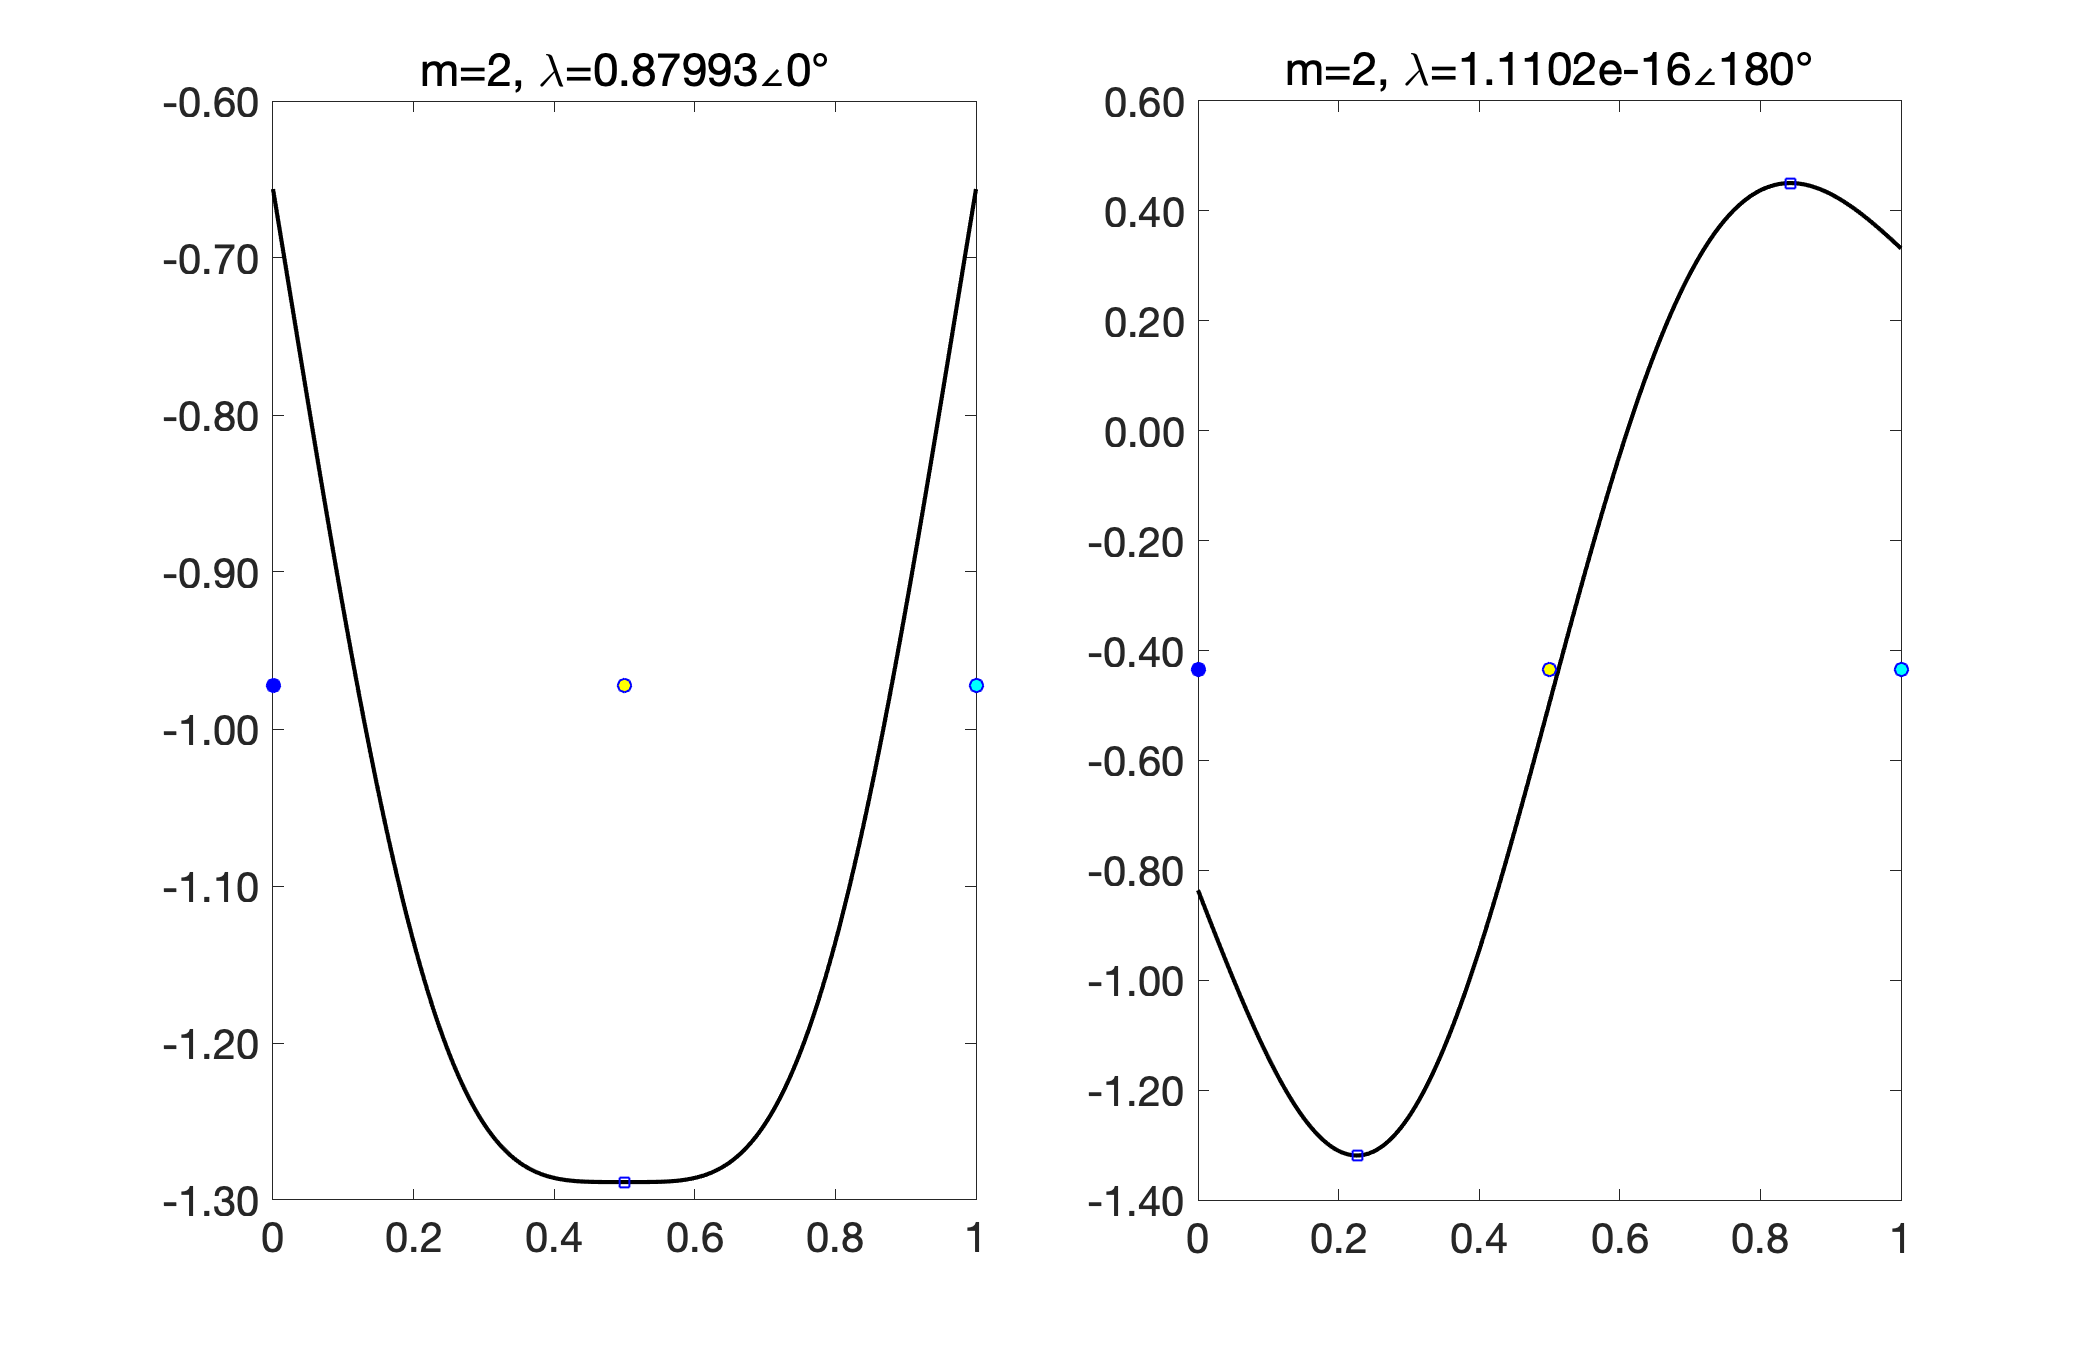
\includegraphics[scale=0.2]{logistic/noise/Logistic_eigen_noise_Gauss_d0_n1000_m2}}
    \subfloat[m=3]{
      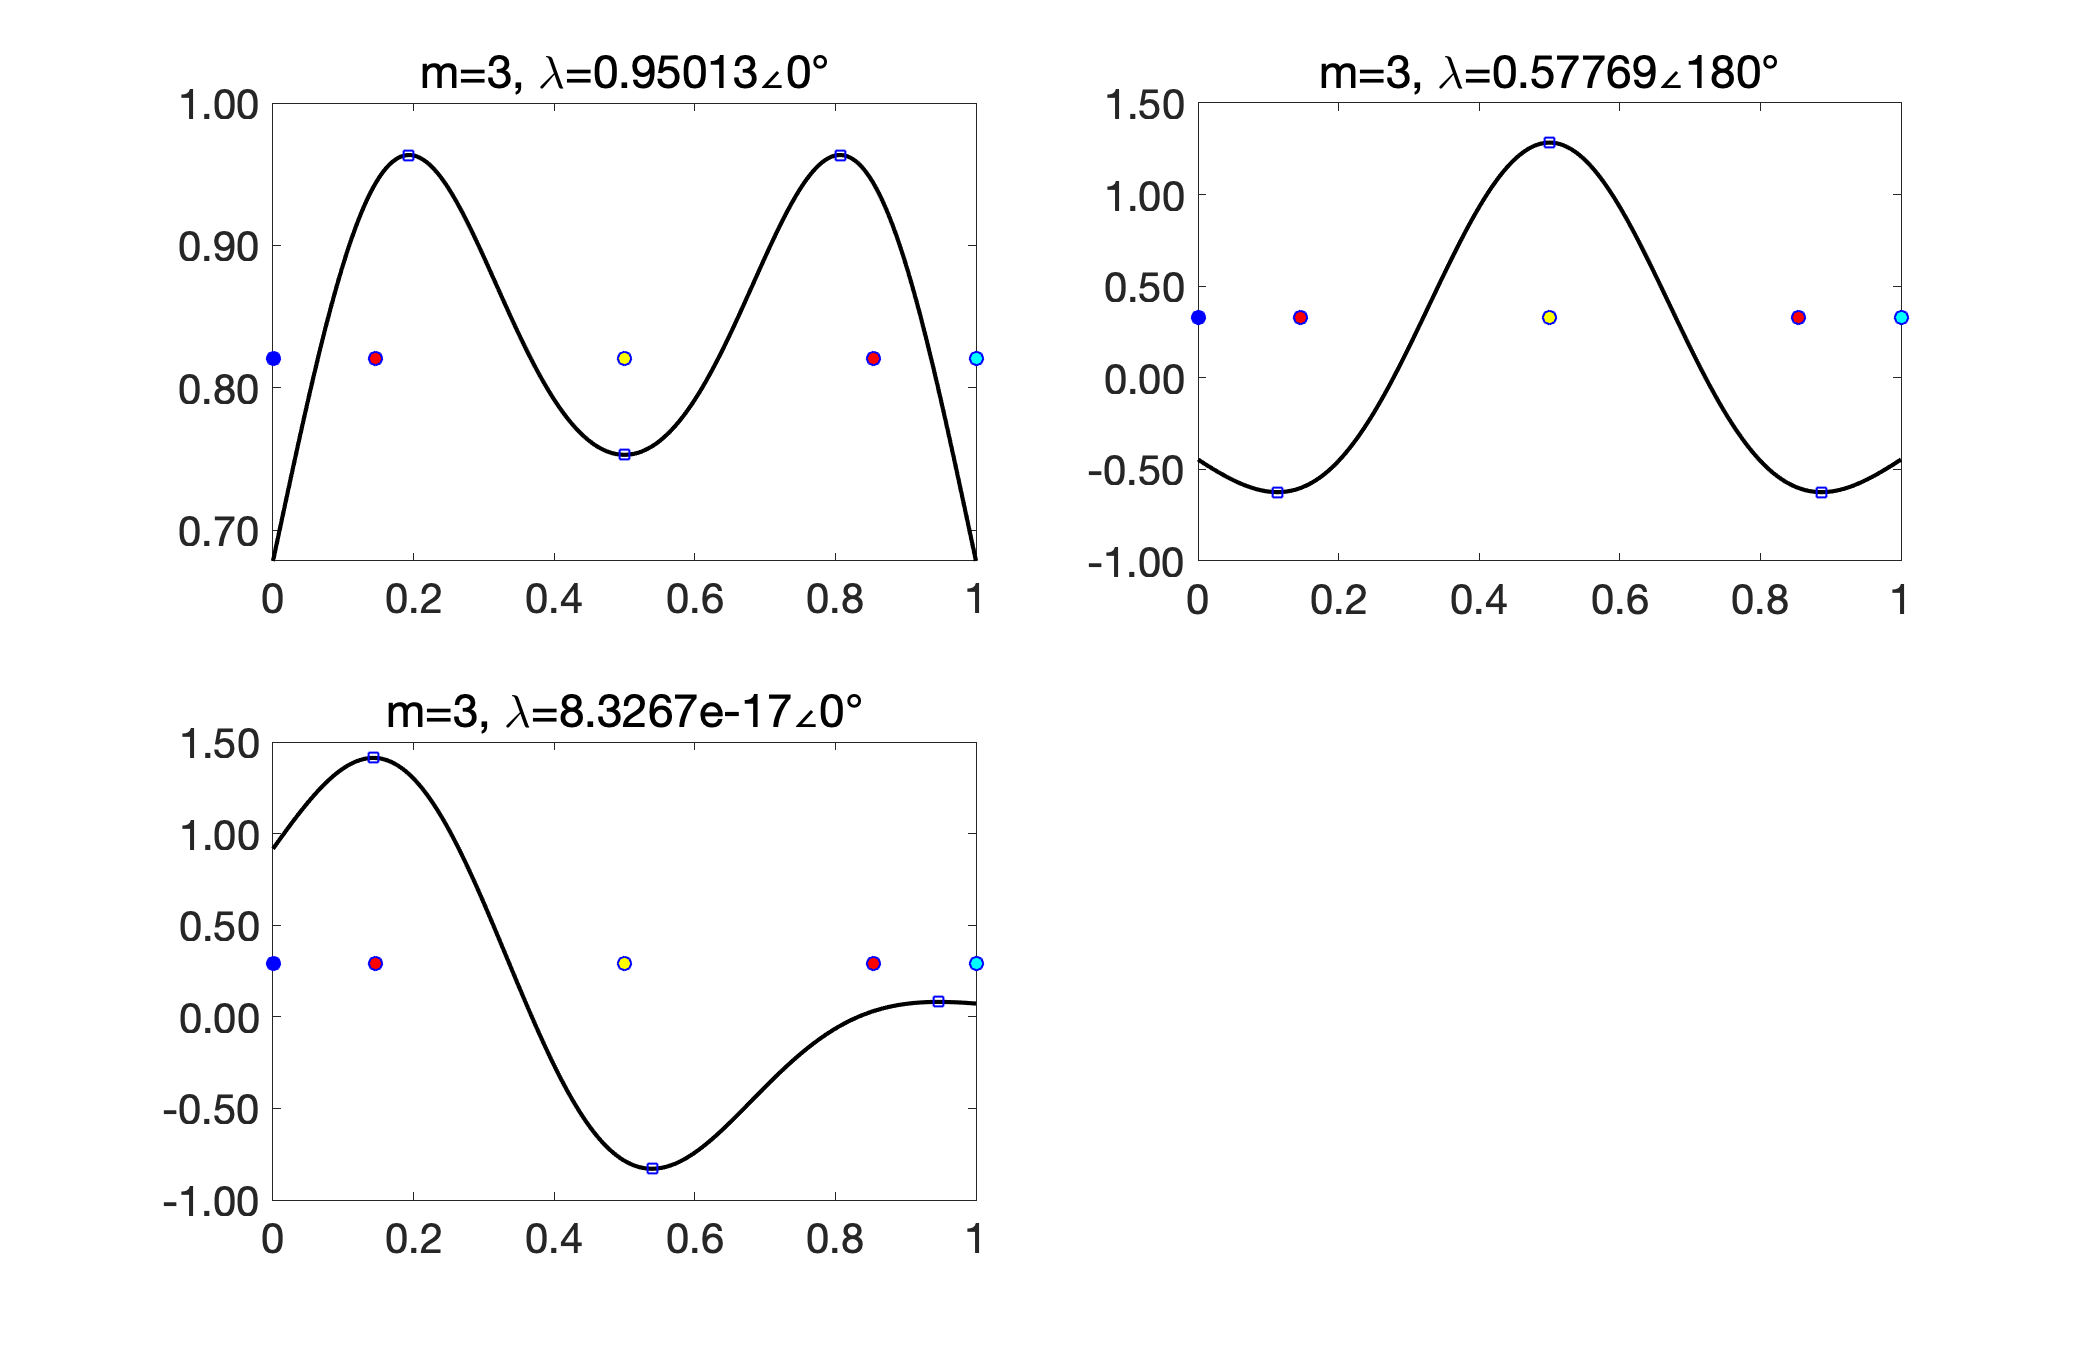
\includegraphics[scale=0.2]{logistic/noise/Logistic_eigen_noise_Gauss_d0_n1000_m3}}
      \\
    \subfloat[m=4]{
      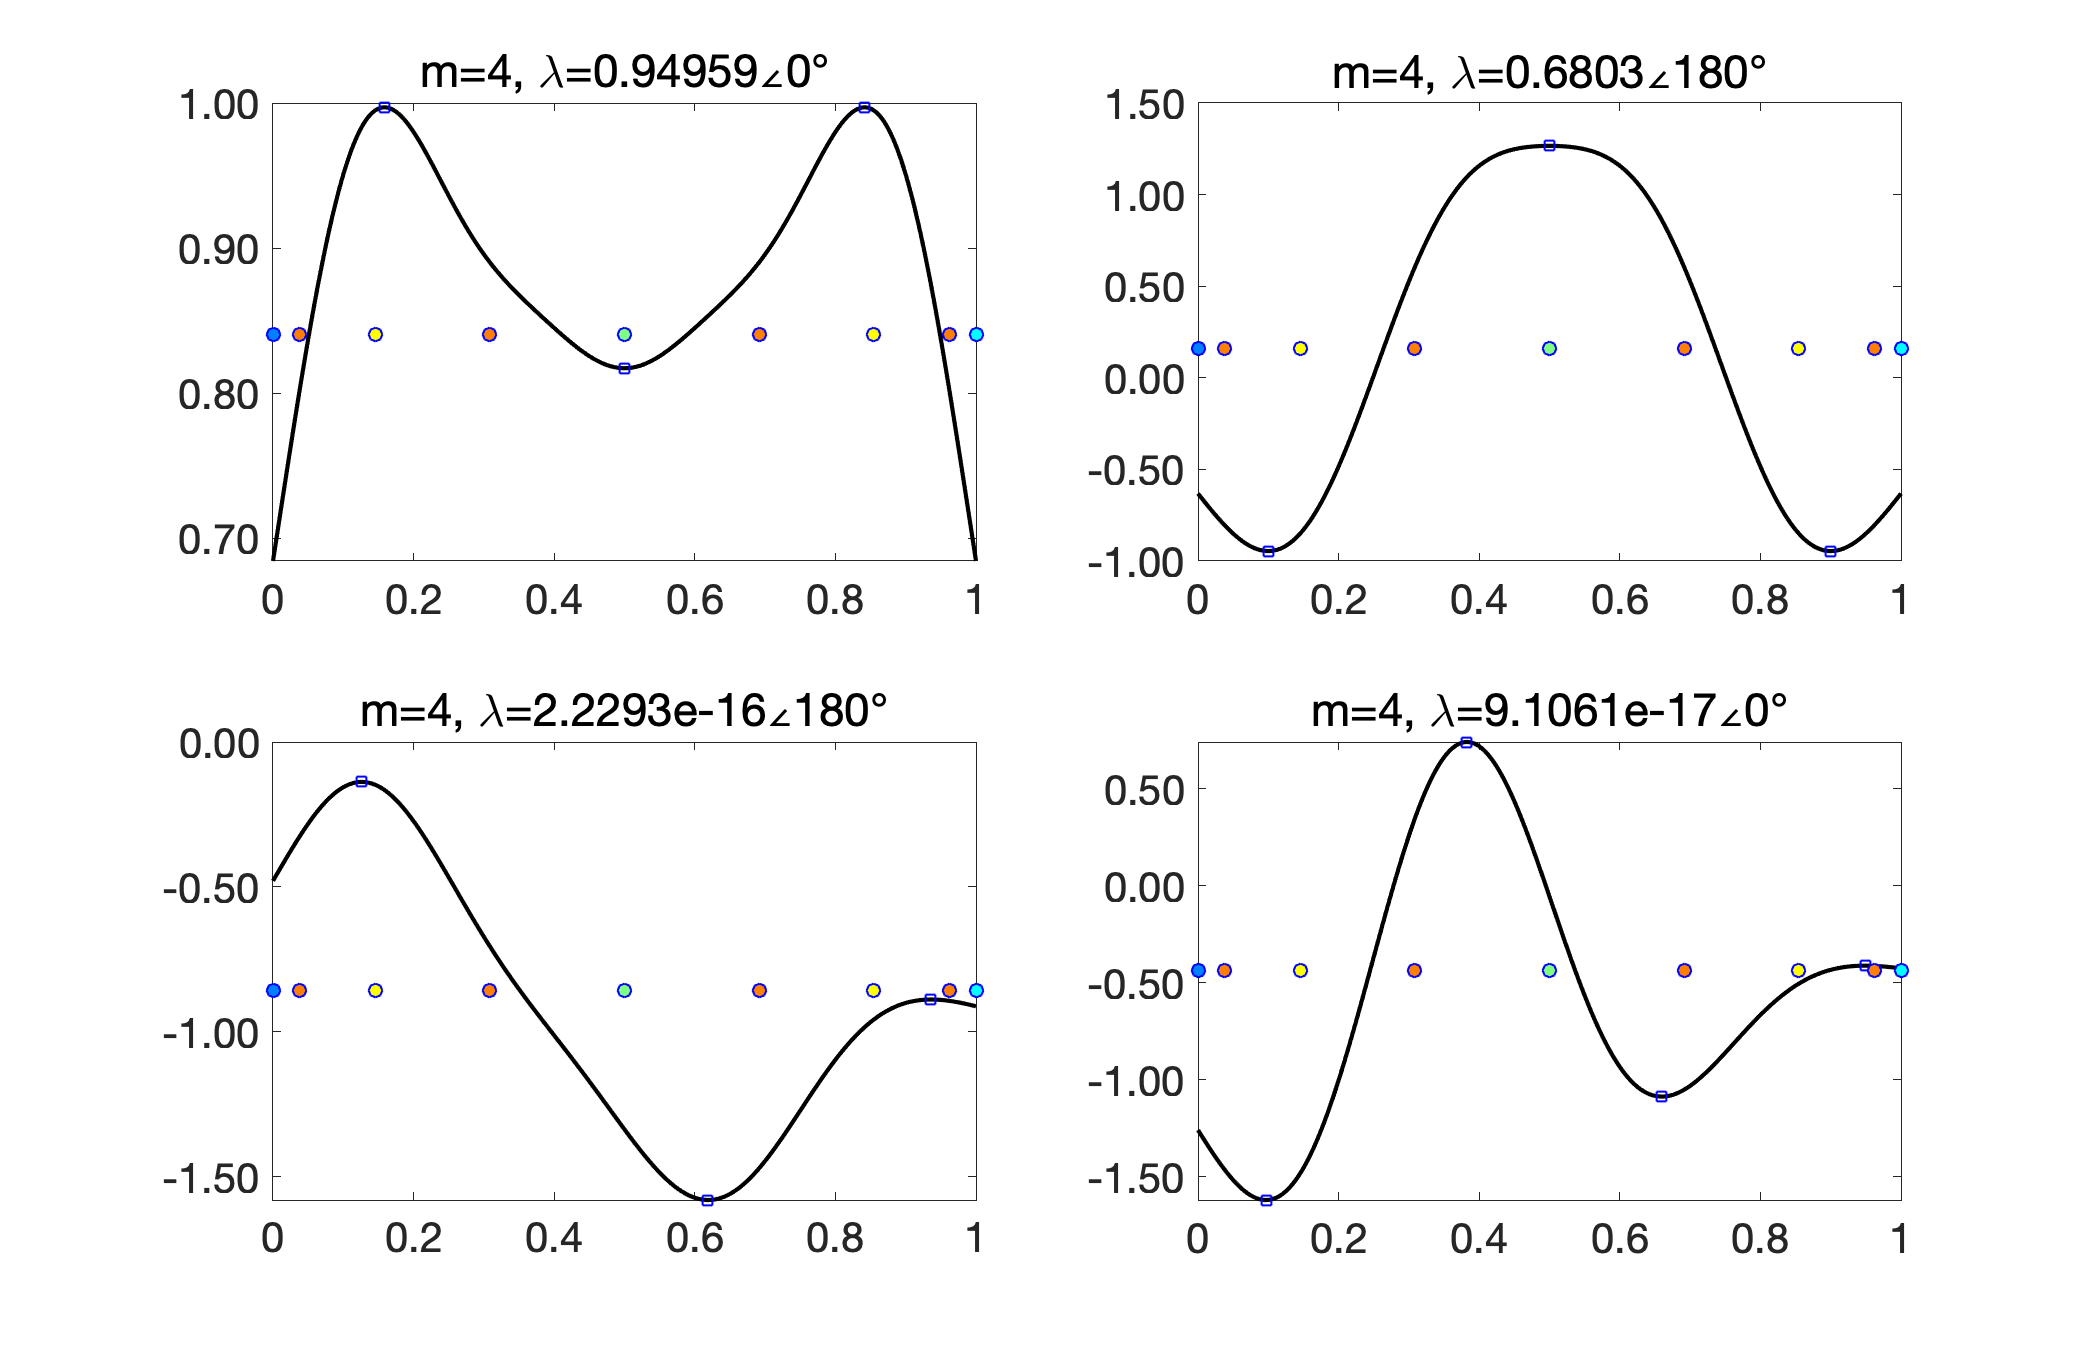
\includegraphics[scale=0.2]{logistic/noise/Logistic_eigen_noise_Gauss_d0_n1000_m4}}
    \subfloat[m=5]{
      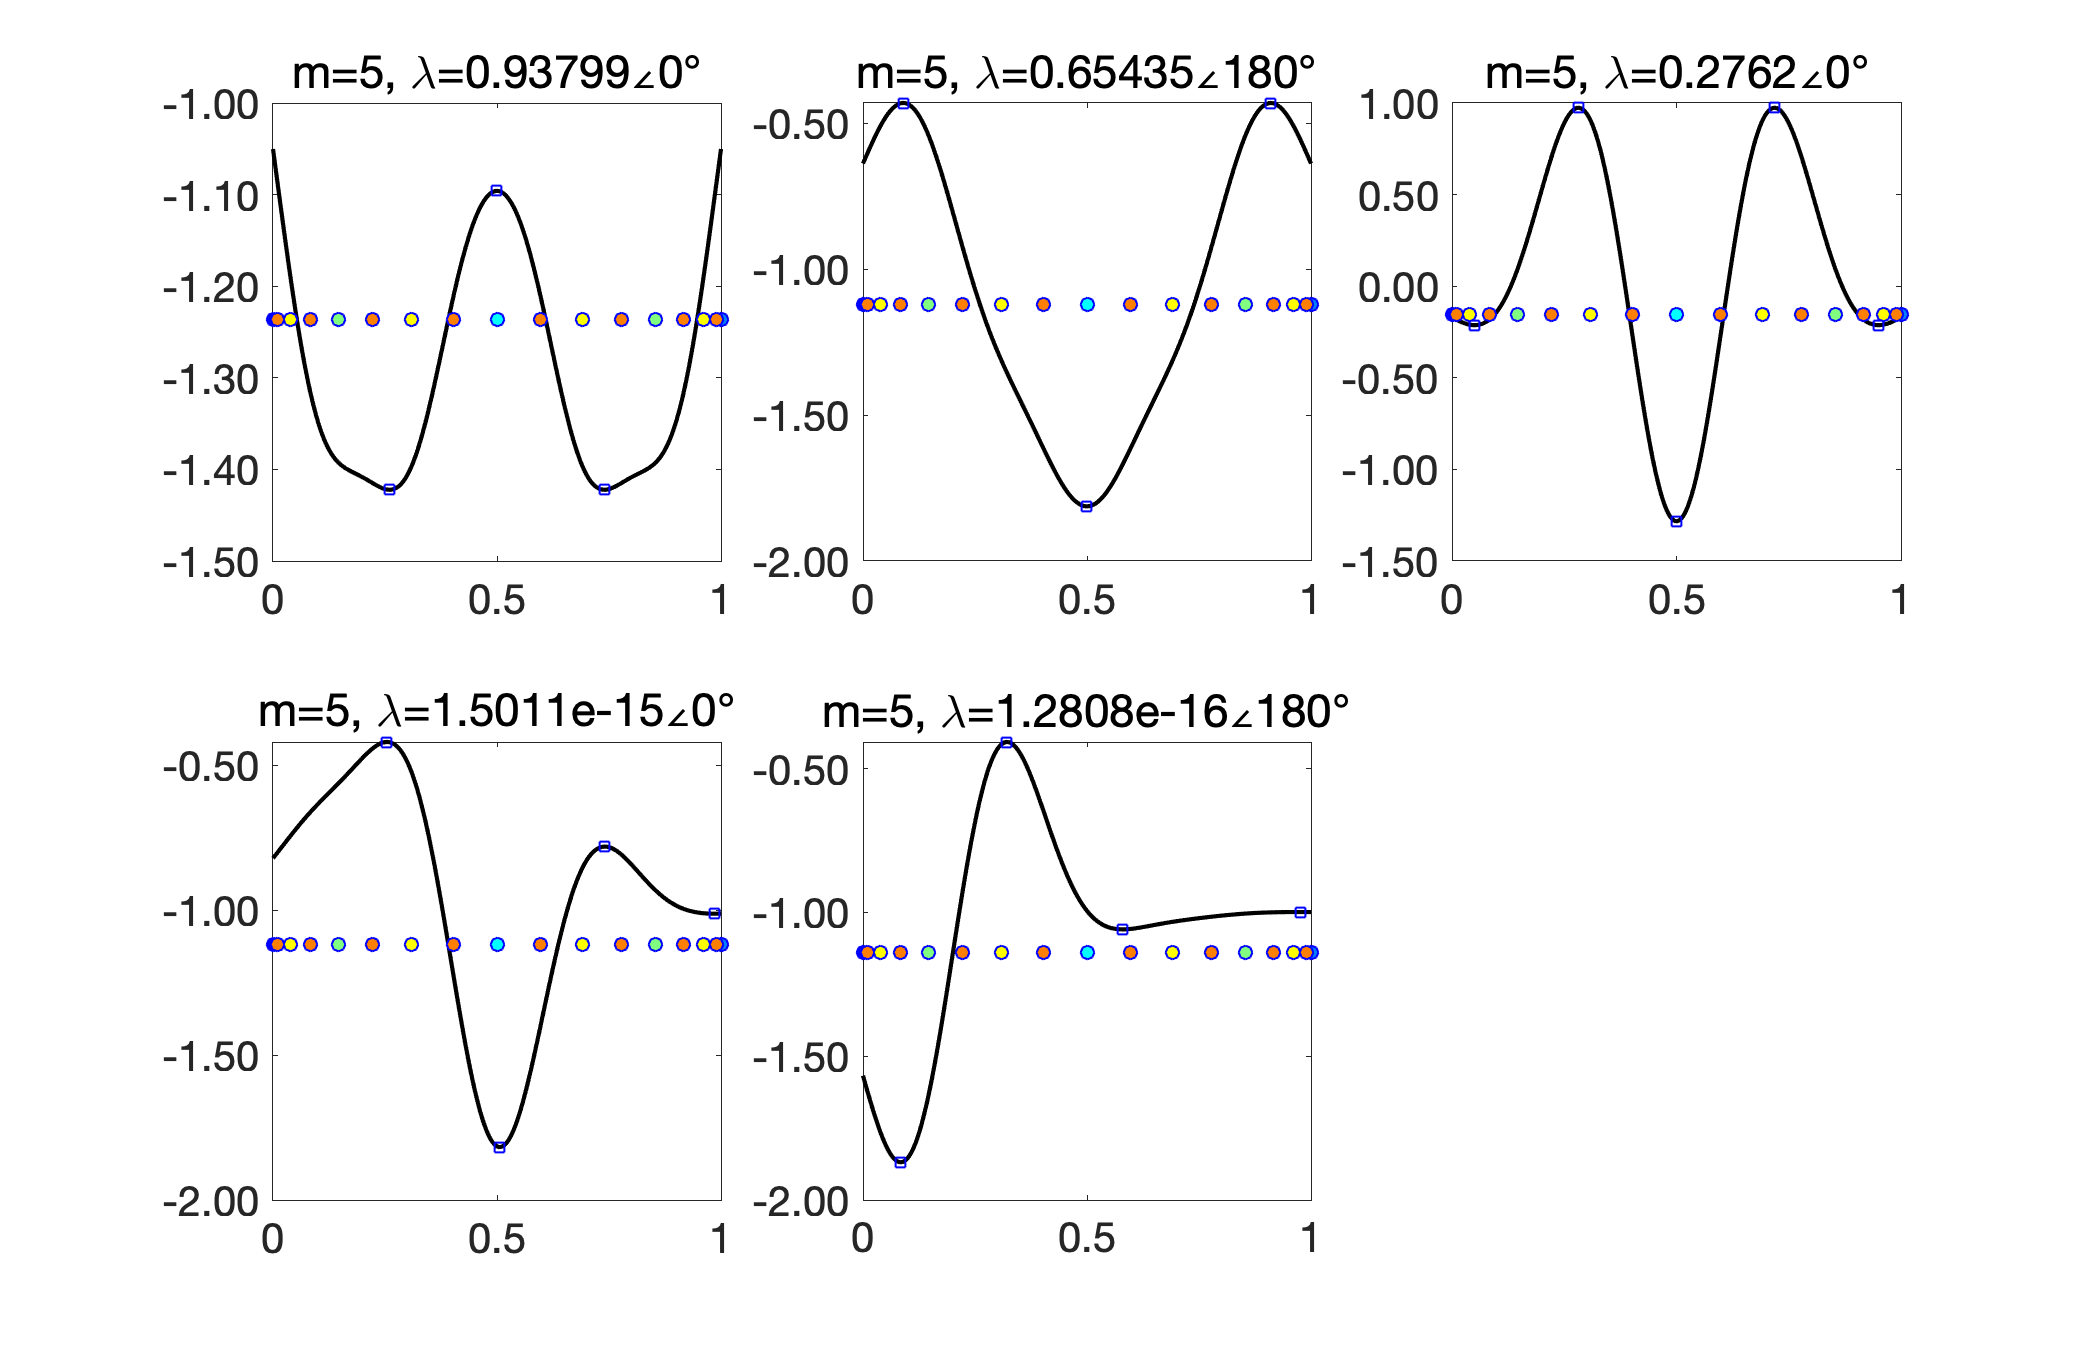
\includegraphics[scale=0.2]{logistic/noise/Logistic_eigen_noise_Gauss_d0_n1000_m5}}
      \\
    \subfloat[m=8]{
      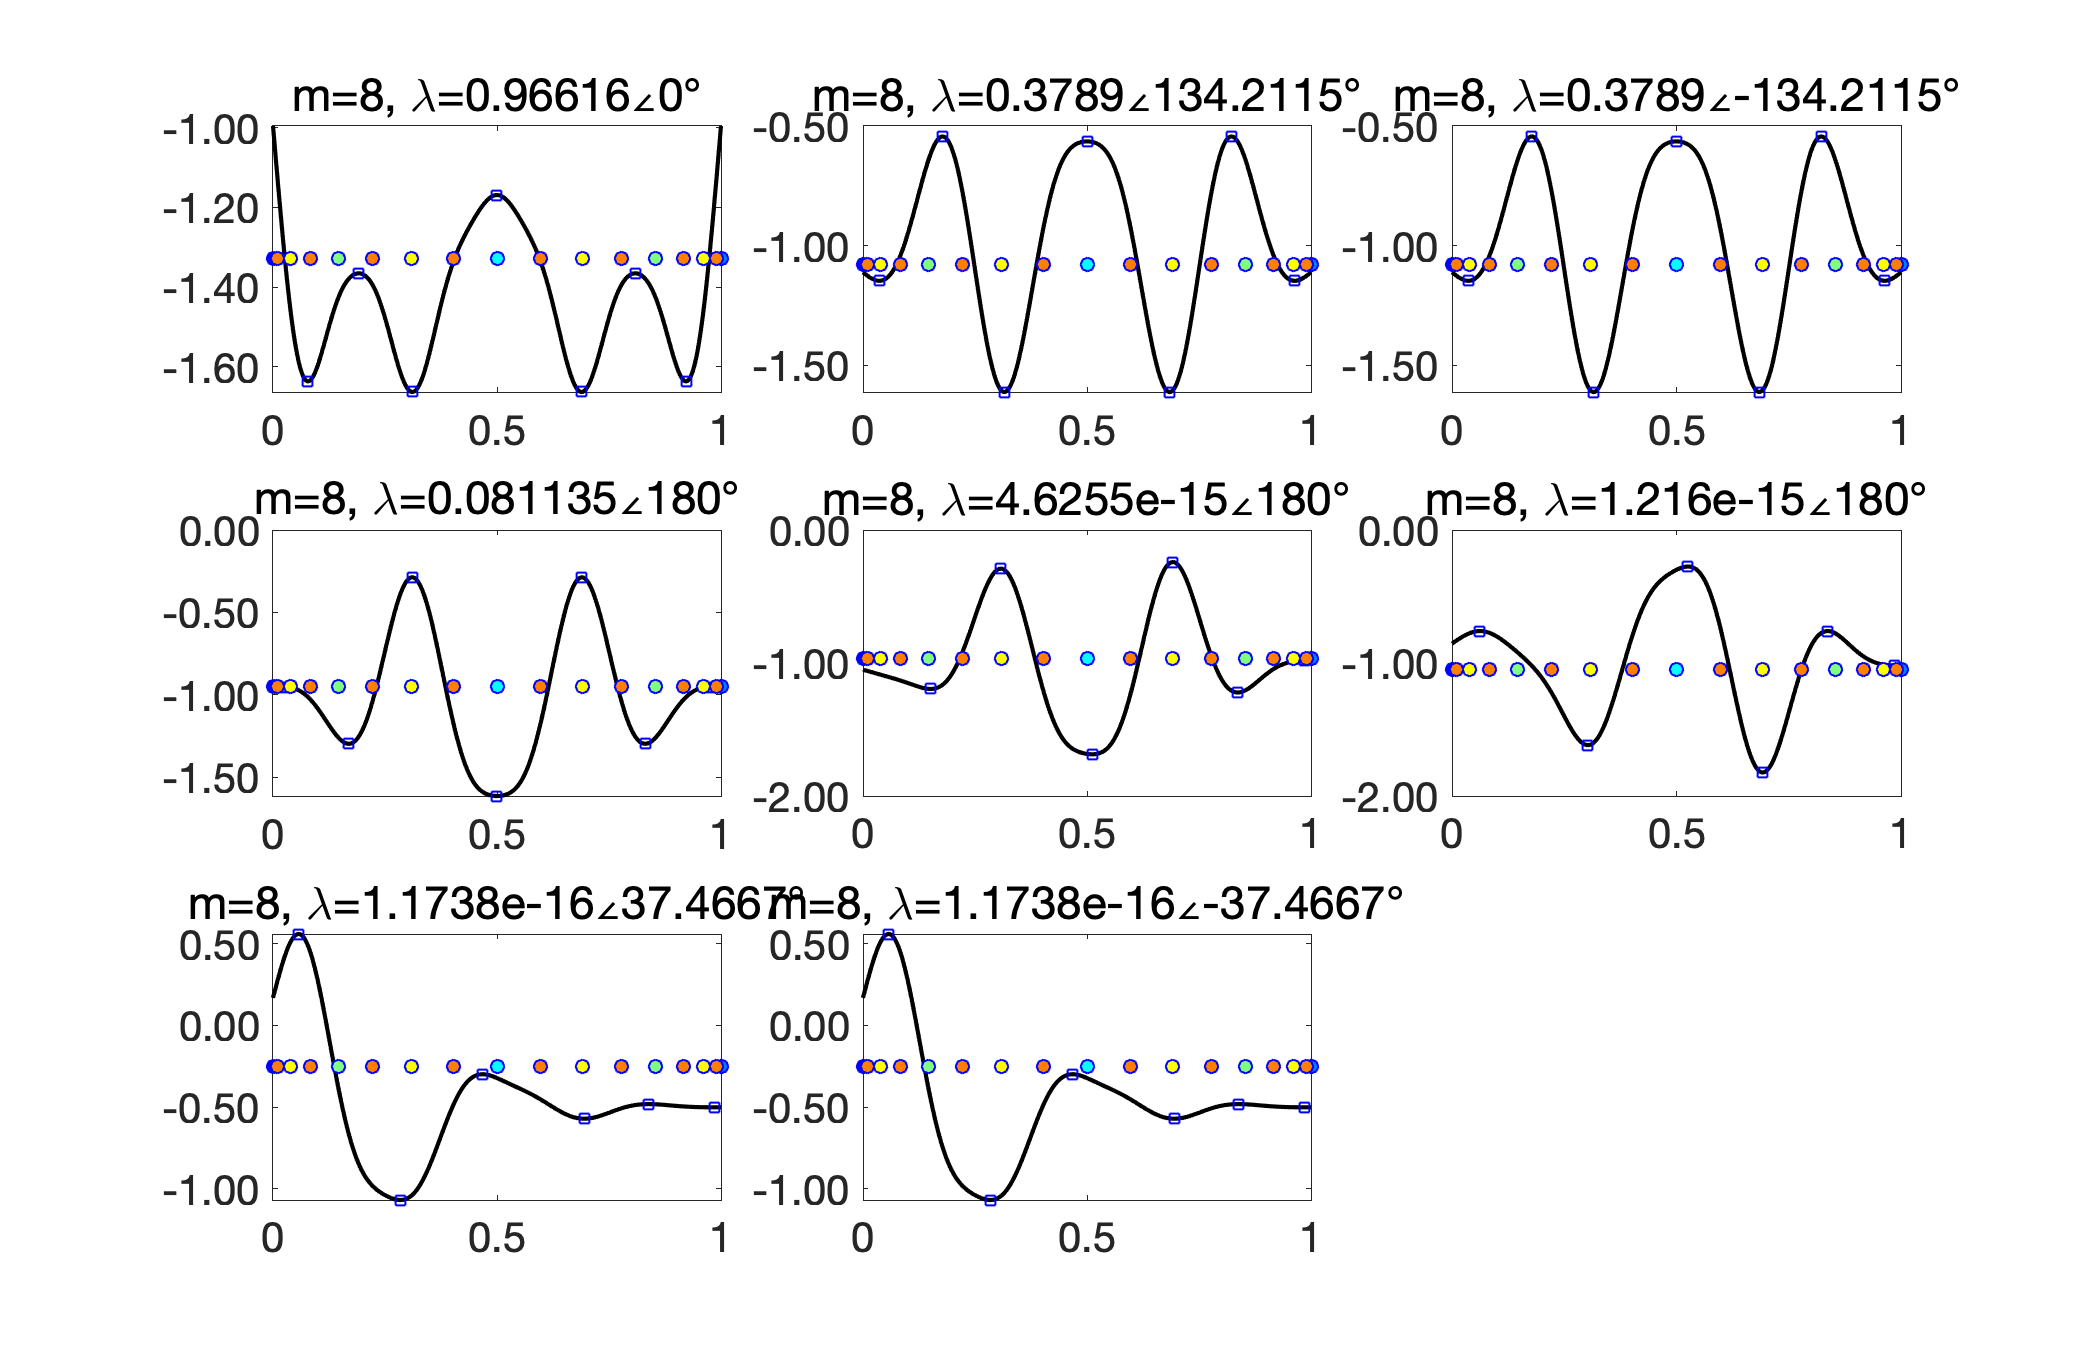
\includegraphics[scale=0.2]{logistic/noise/Logistic_eigen_noise_Gauss_d0_n1000_m8}}
    \subfloat[m=10]{
      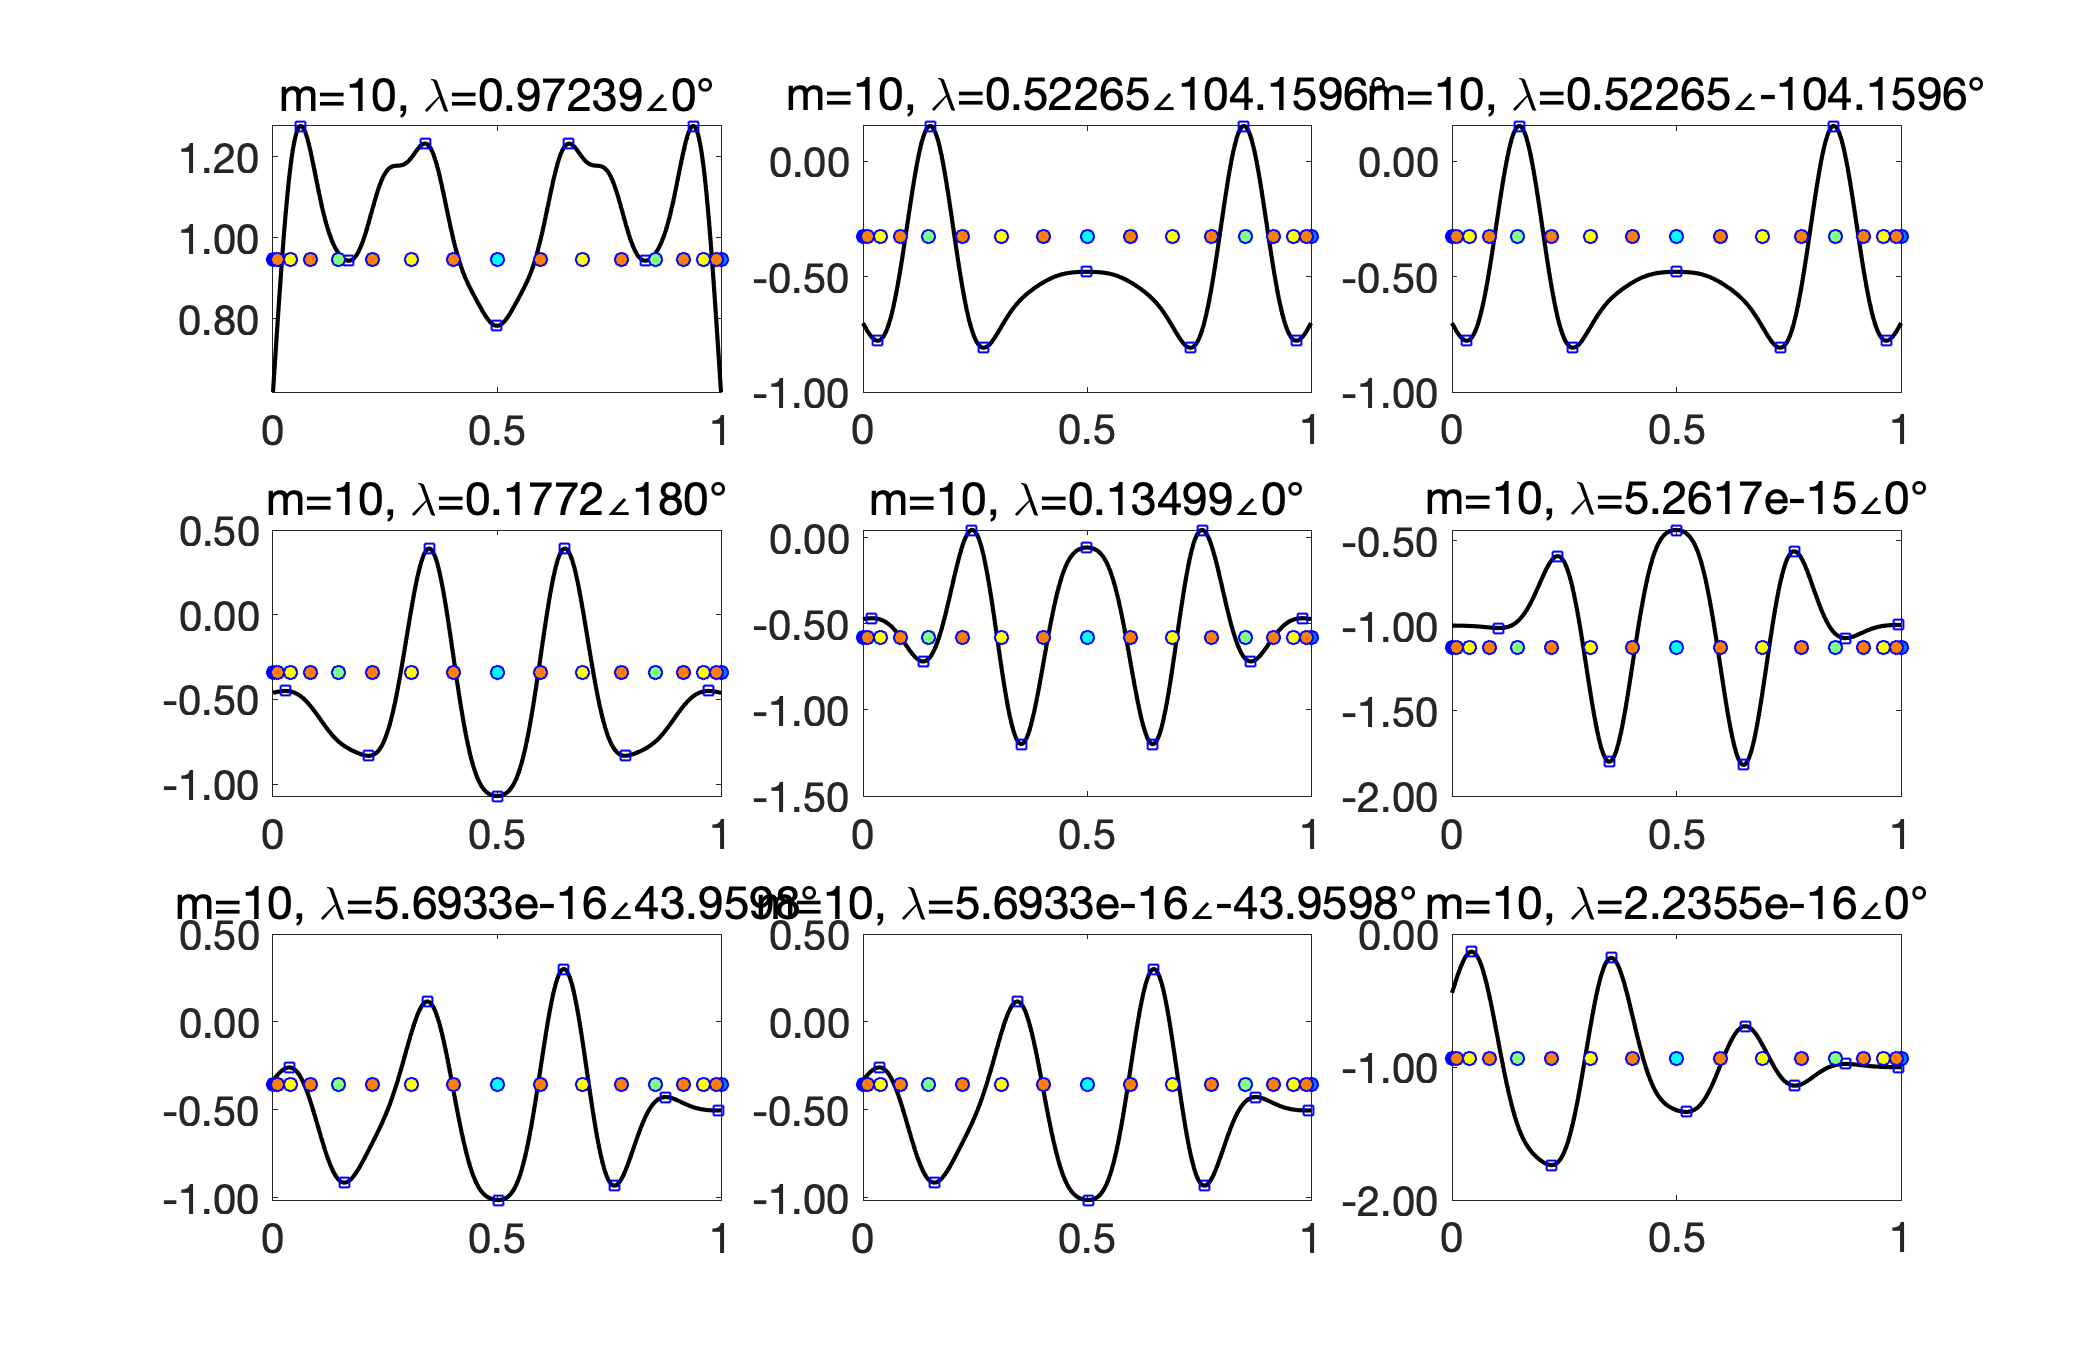
\includegraphics[scale=0.2]{logistic/noise/Logistic_eigen_noise_Gauss_d0_n1000_m10}}
      \\
    \subfloat[m=15]{
      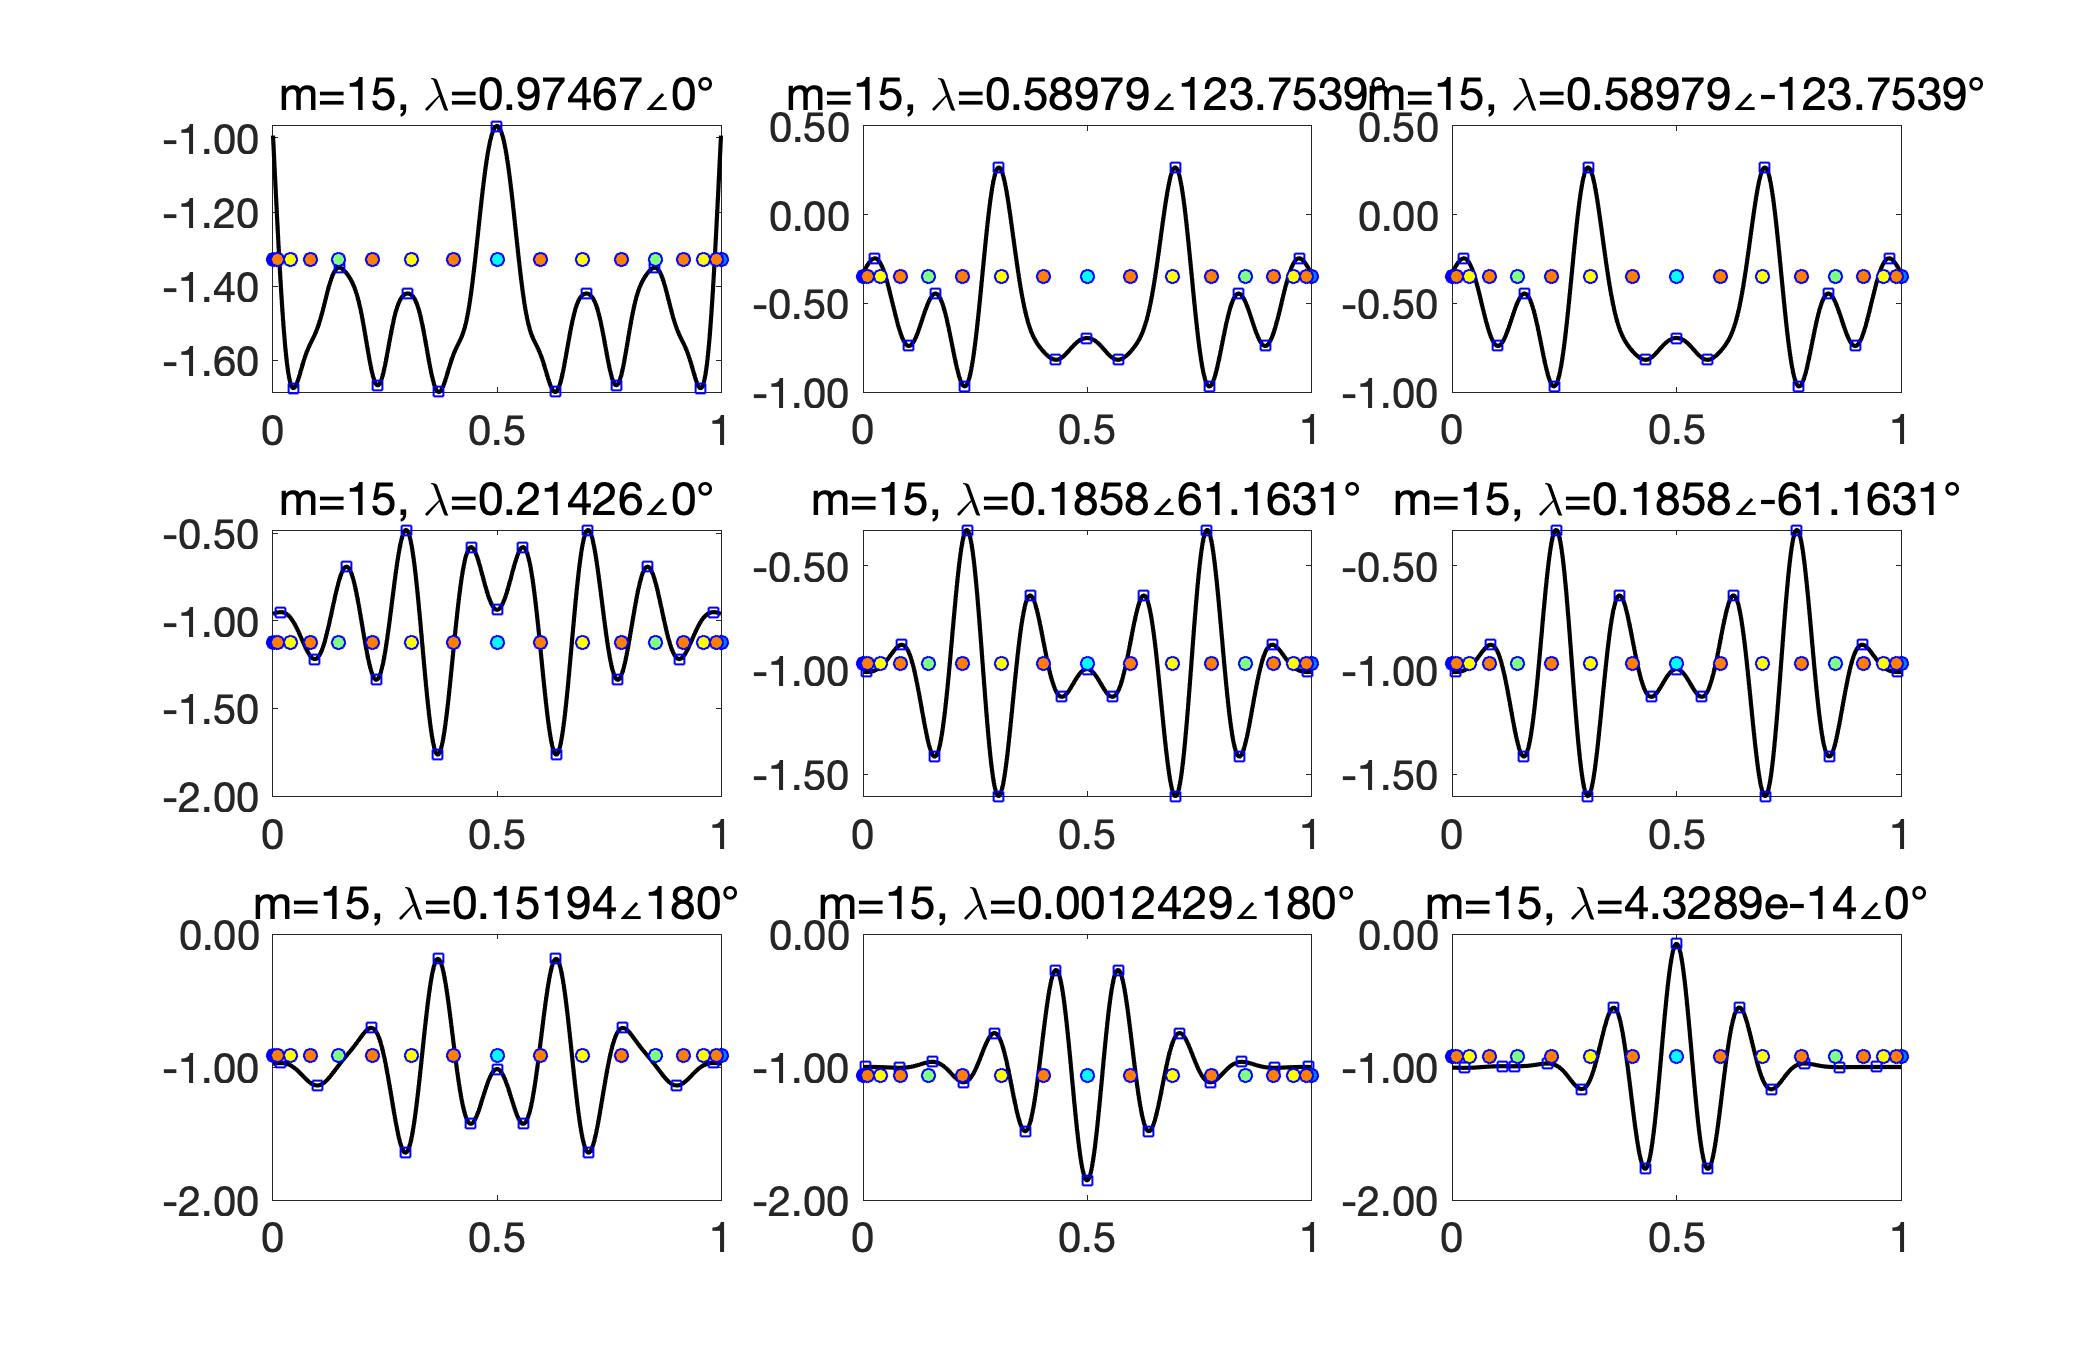
\includegraphics[scale=0.2]{logistic/noise/Logistic_eigen_noise_Gauss_d0_n1000_m15}}
    \subfloat[m=20]{
      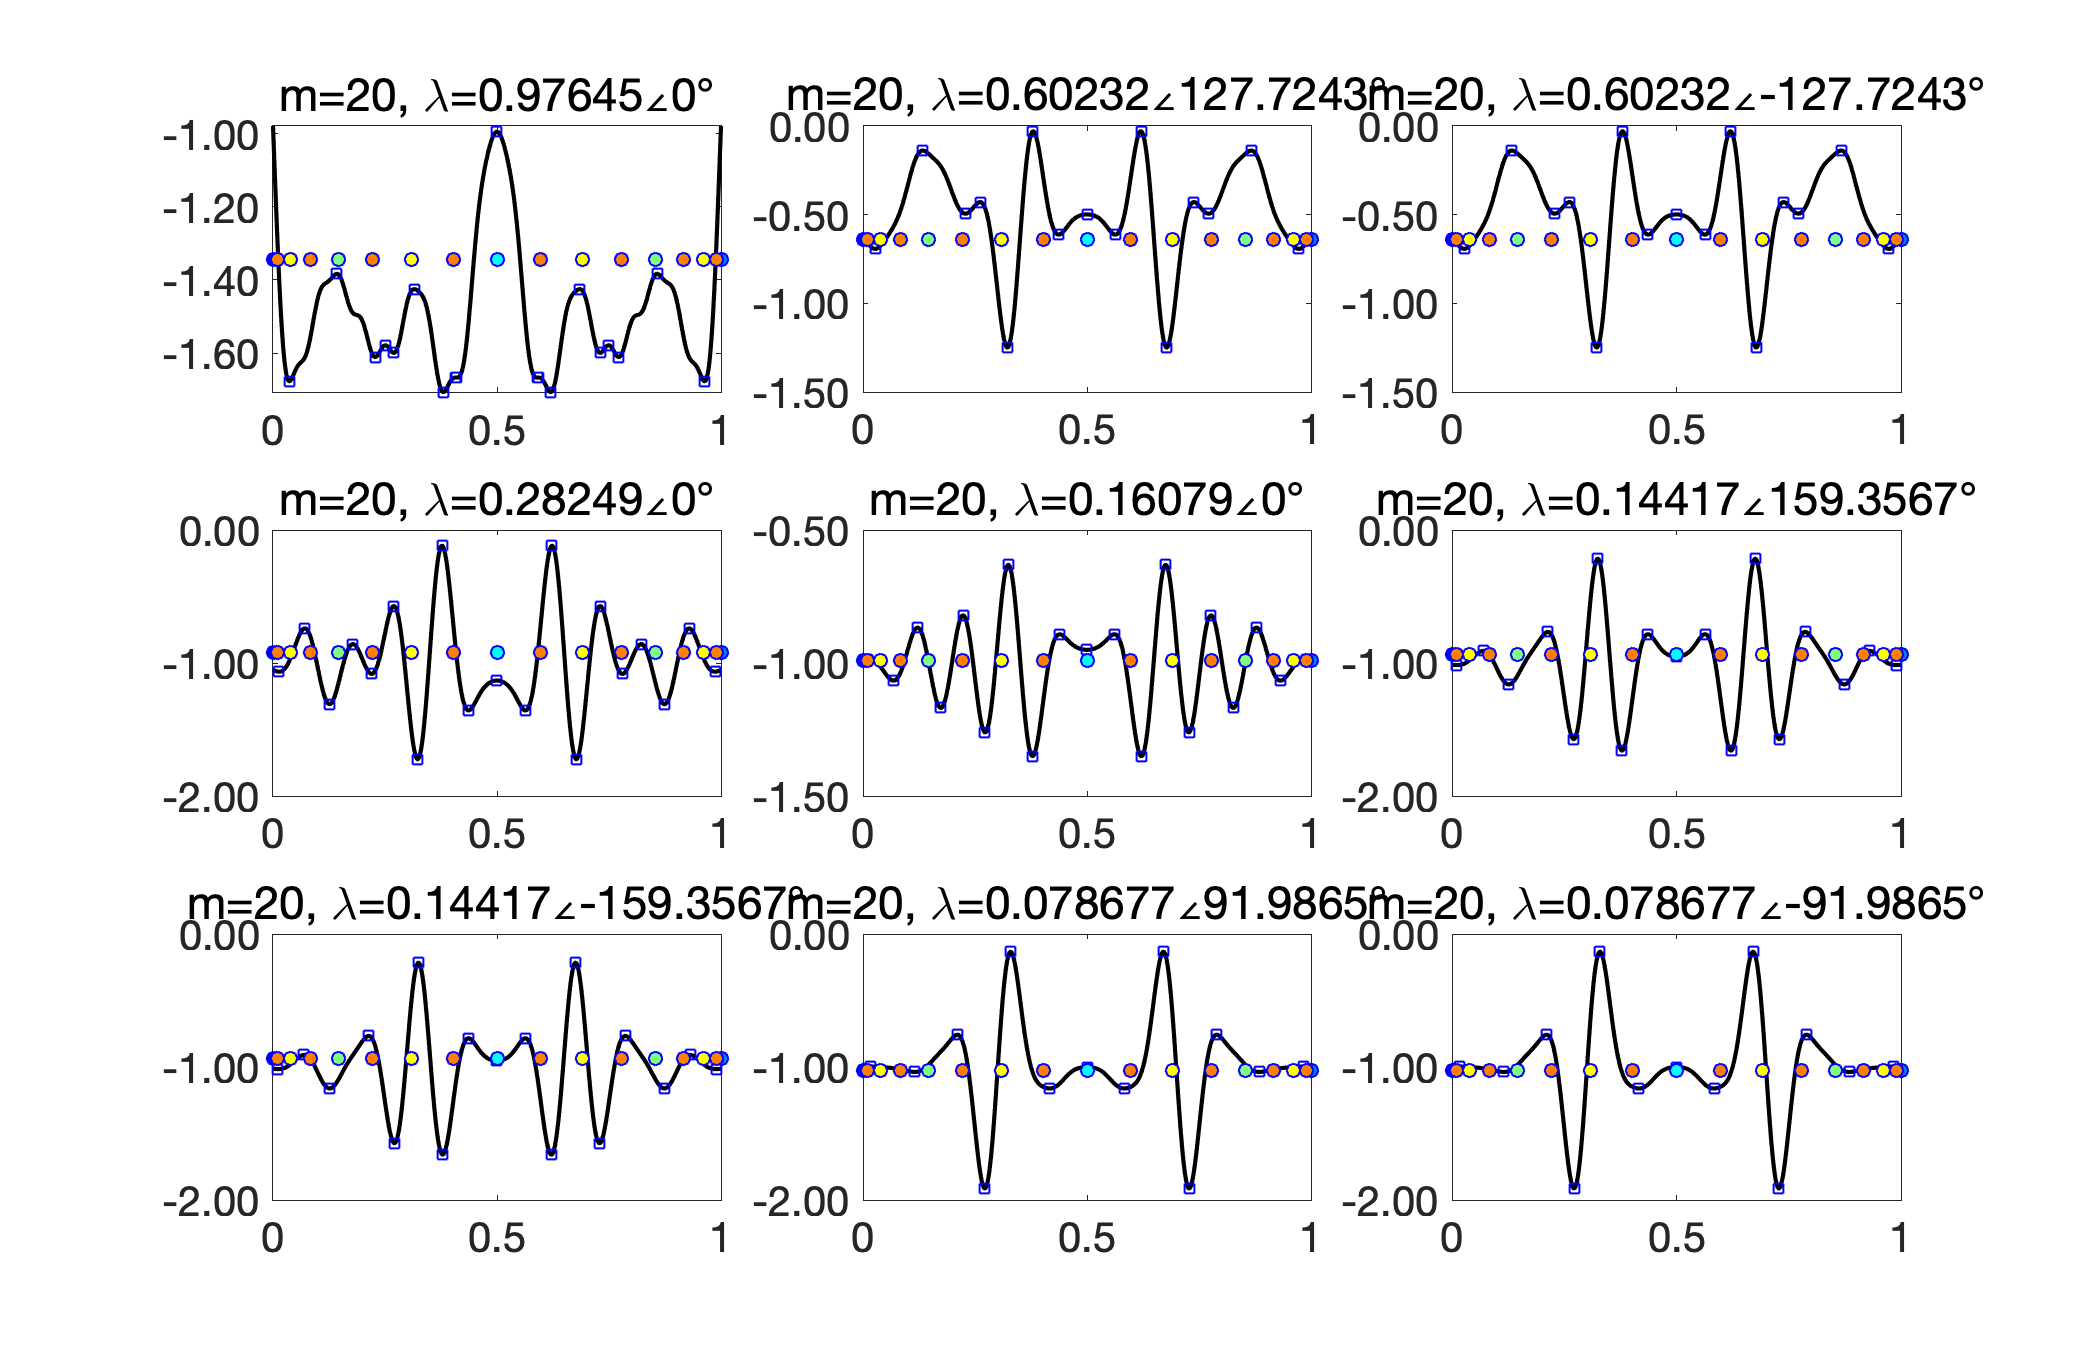
\includegraphics[scale=0.2]{logistic/noise/Logistic_eigen_noise_Gauss_d0_n1000_m20}}
      \\
    \caption[Logistic映射的边界点与本征函数]{Logistic映射的边界点与本征函数:每个图中不同颜色的点表示不同层次的边界点,且本征函数的极值点用空心方块标出}\label{fig:Logistic_eigen_noise_n1000m2d0}
  \end{figure}

  我们观察本征函数的极值点与Logistic的边界点,在图\ref{fig:Tent_eigen_noise_n1000m2d0}(a)的第二个小图中,我们观察到基函数$m=2$时本征函数存在一个极值点,其与边界点$x=\frac{1}{2}$是比较吻合的。随着基函数数量的增加$m=3,4,5,8,10$时,$x=0.1464,0.8536$处附近的极值点越来越逼近这两个边界点,当$m=15$时,$x=0.1464,0.8536$处附近各存在一个极值点;当$m=20$时,极值点与边界点吻合的较好。

  结合帐篷映射我们可以得出与之一致的结论:Koopman算符的本征函数的极值点反映了Logistic映射的边界点,且随着本征函数基函数数量的增加,函数格点的增加使本征函数的精细度增加,从而能更精确的刻画Logistic映射的边界点;我们可以依本征函数的极值点对相空间区域进行划分;Koopman算符的本征函数极值点可以反映符号动力学的分界点。
  
  通过帐篷映射与Logistic映射中一致的结论,我们可以大胆的将此结论应用到更复杂的系统中,当我们面对一个较复杂的系统时,我们可以通过Koopman算符的本征函数寻找其极值点,来寻找该系统对应的符号动力学的分界点。且随着我们增加基函数的数量,我们便能更精细的刻画符号动力学的分界点。从而使我们对该动力学的特征能够有着粗粒度的认识。

\subsection{更多的讨论}

在帐篷映射中我们对Koopman算符的本征函数的极值点反映了帐篷映射的边界点的结论作了一定的探究,为了揭示此规律的普遍性,在本小节中我们将对噪声下的Logistic映射和寻找更精细的边界点这两个问题进行讨论,同时与帐篷映射进行对比。

在噪声情况下,假设我们的涨落符合高斯白噪声分布,将Logistic映射加入噪声项得到含噪声的Logistic映射:
\begin{equation}
  x_{n+1}=f(x_n)=\gamma x_n(1-x_n)+\xi
\end{equation}
其中高斯分布的方差作为信噪比的参数可供调节,Logistic映射在不同噪声大小下的相图如图\ref{fig:Logistic_noise_phase_d0}所示。若Koopman算符对边界点的划分具有鲁棒性,则在此噪声影响下,Koopman算符对边界点的划分应与之前相同。


\begin{figure}[!]
    \centering
    \subfloat[noise=0]{
      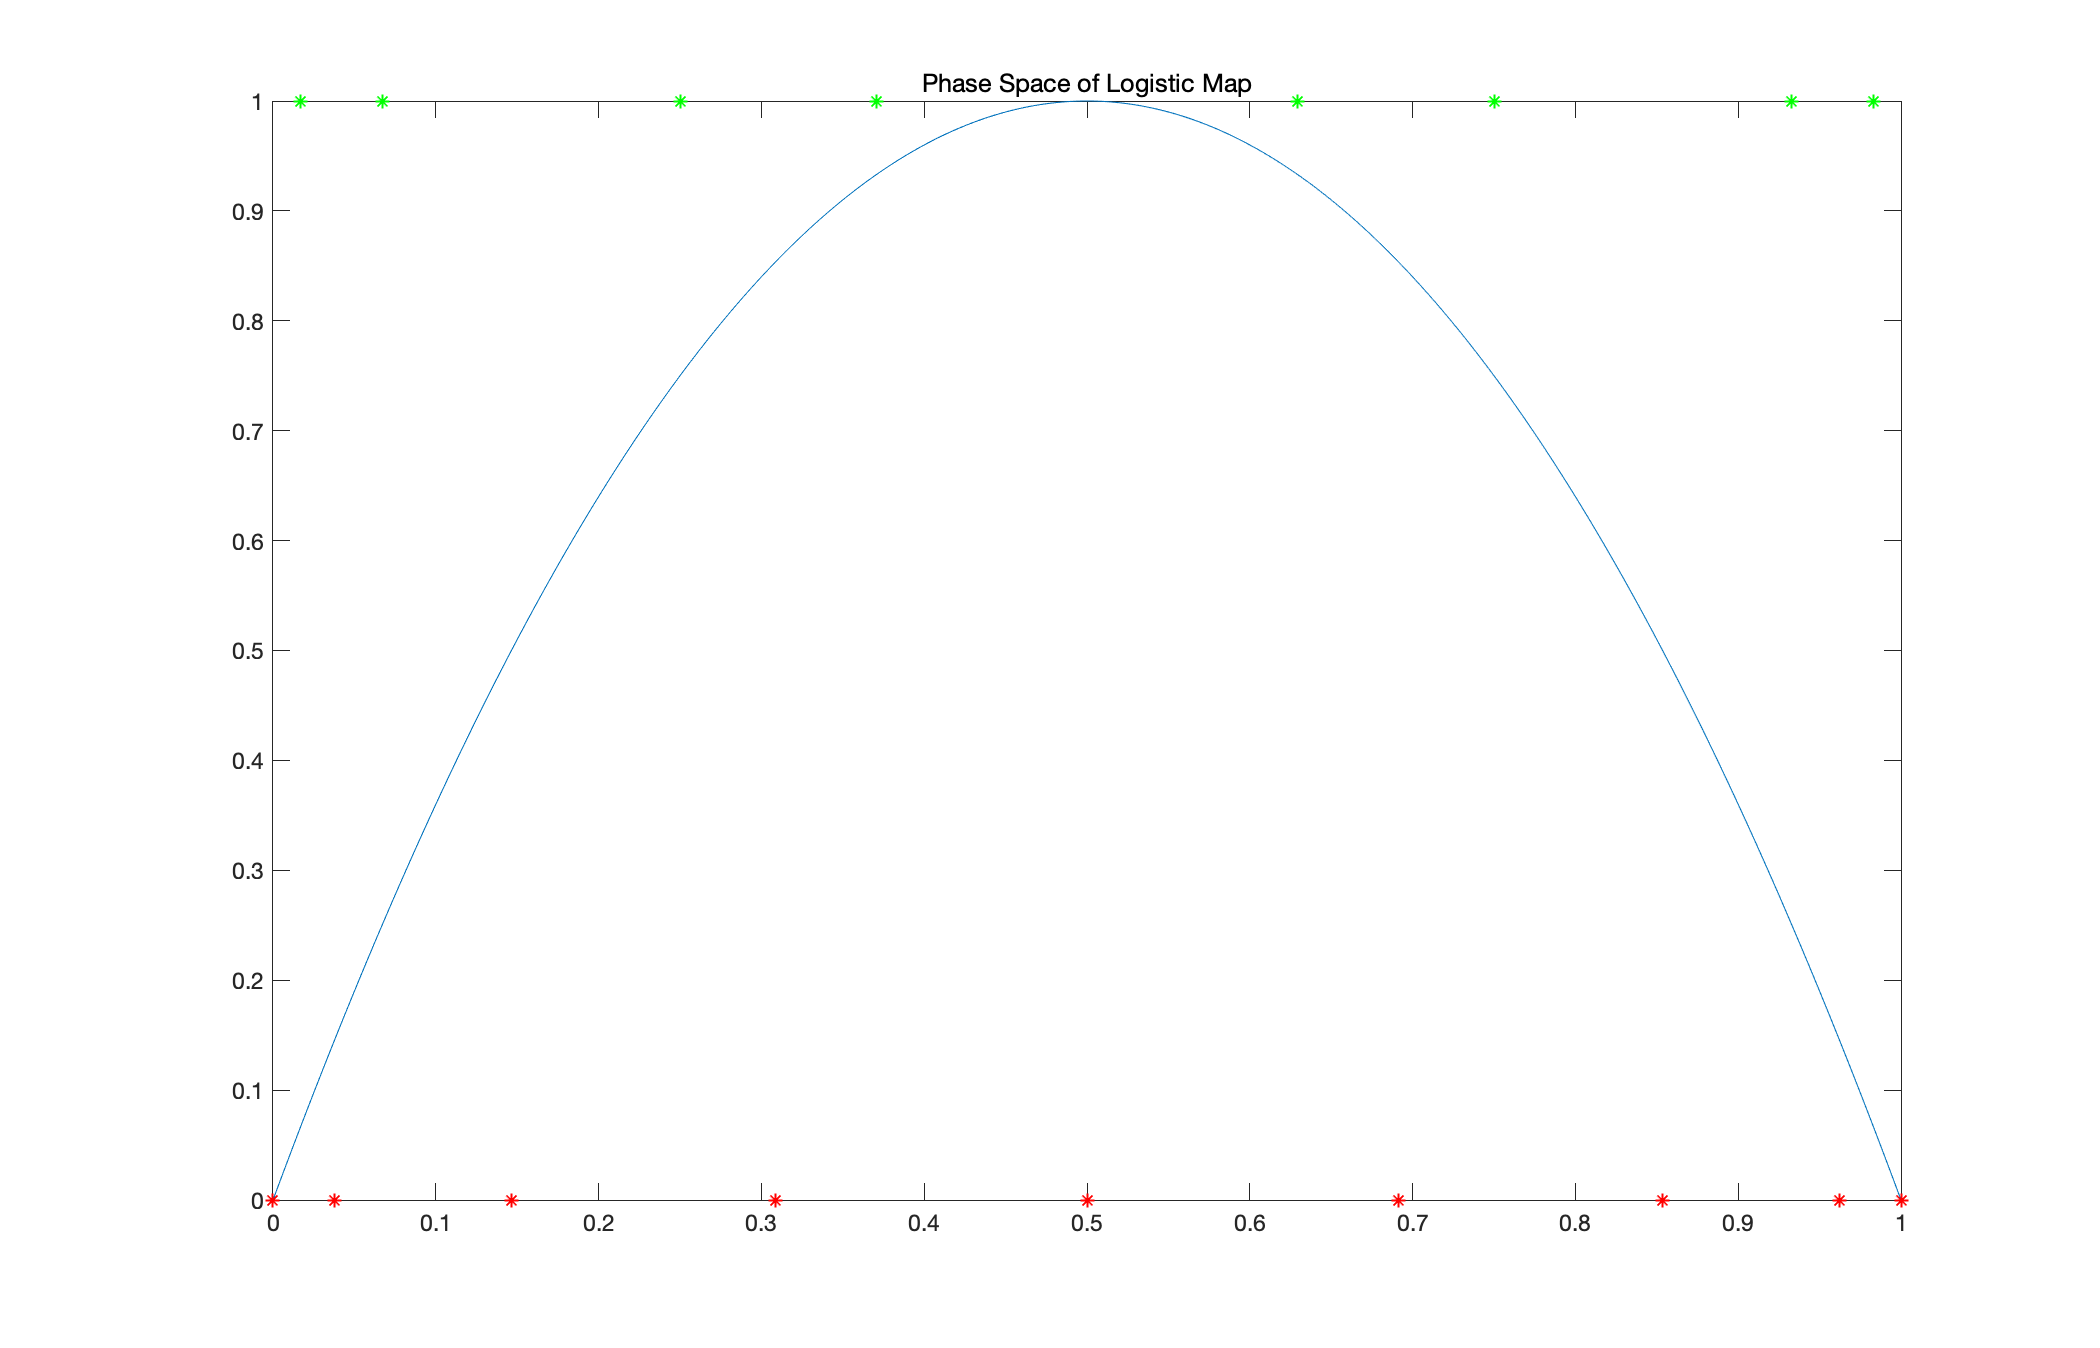
\includegraphics[scale=0.13]{logistic/noise/Logistic_noise_phase_d0}}
    \subfloat[noise=0.001]{
      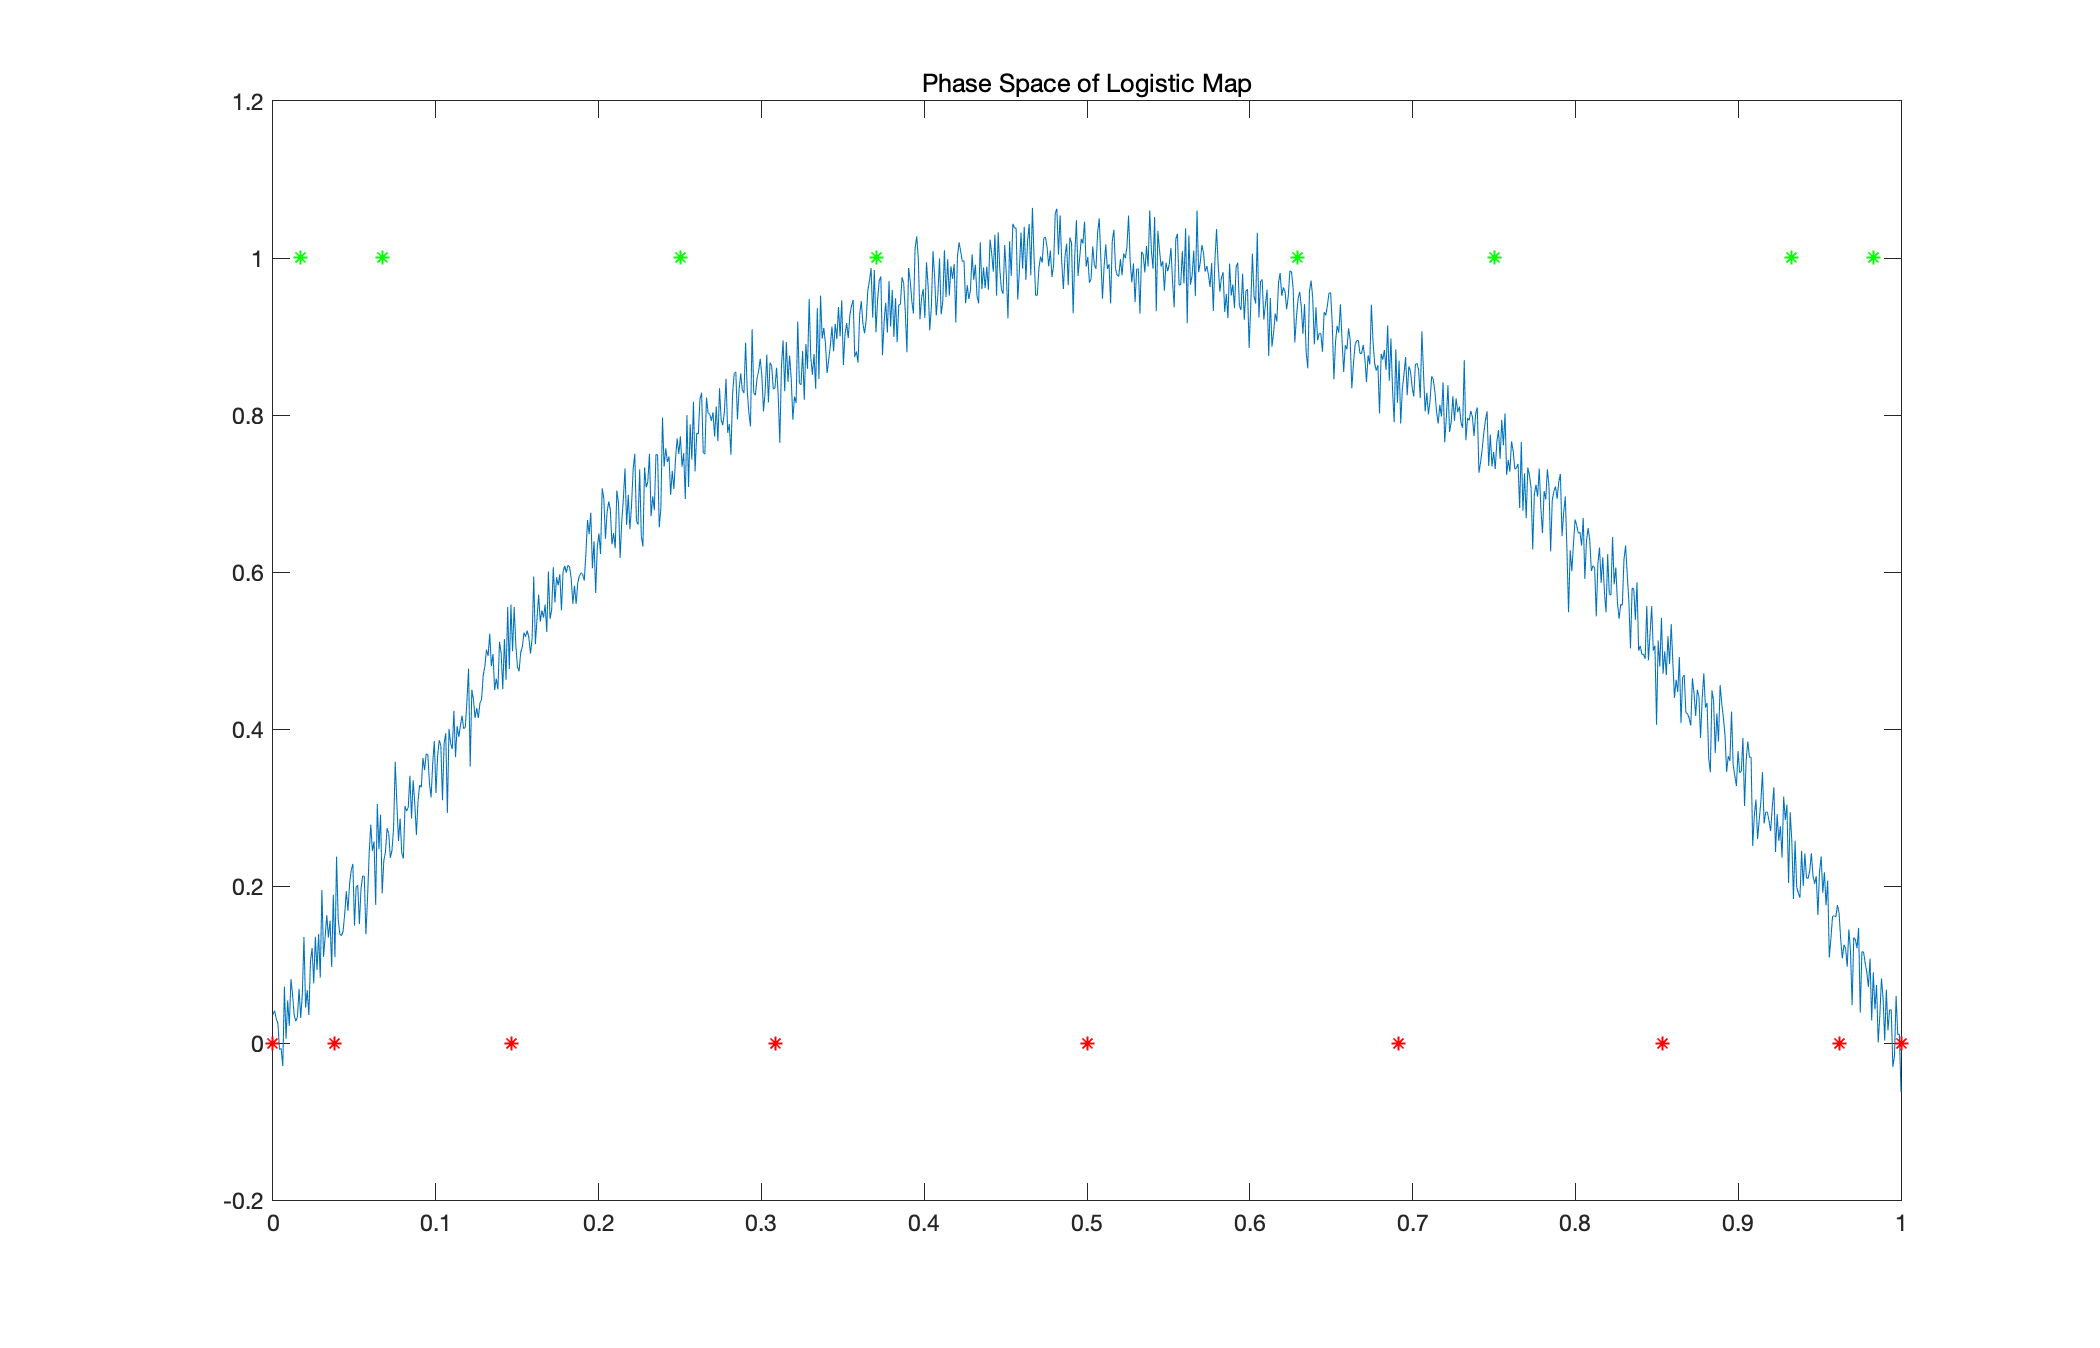
\includegraphics[scale=0.13]{logistic/noise/Logistic_noise_phase_d0-001}}
    \subfloat[noise=0.01]{
      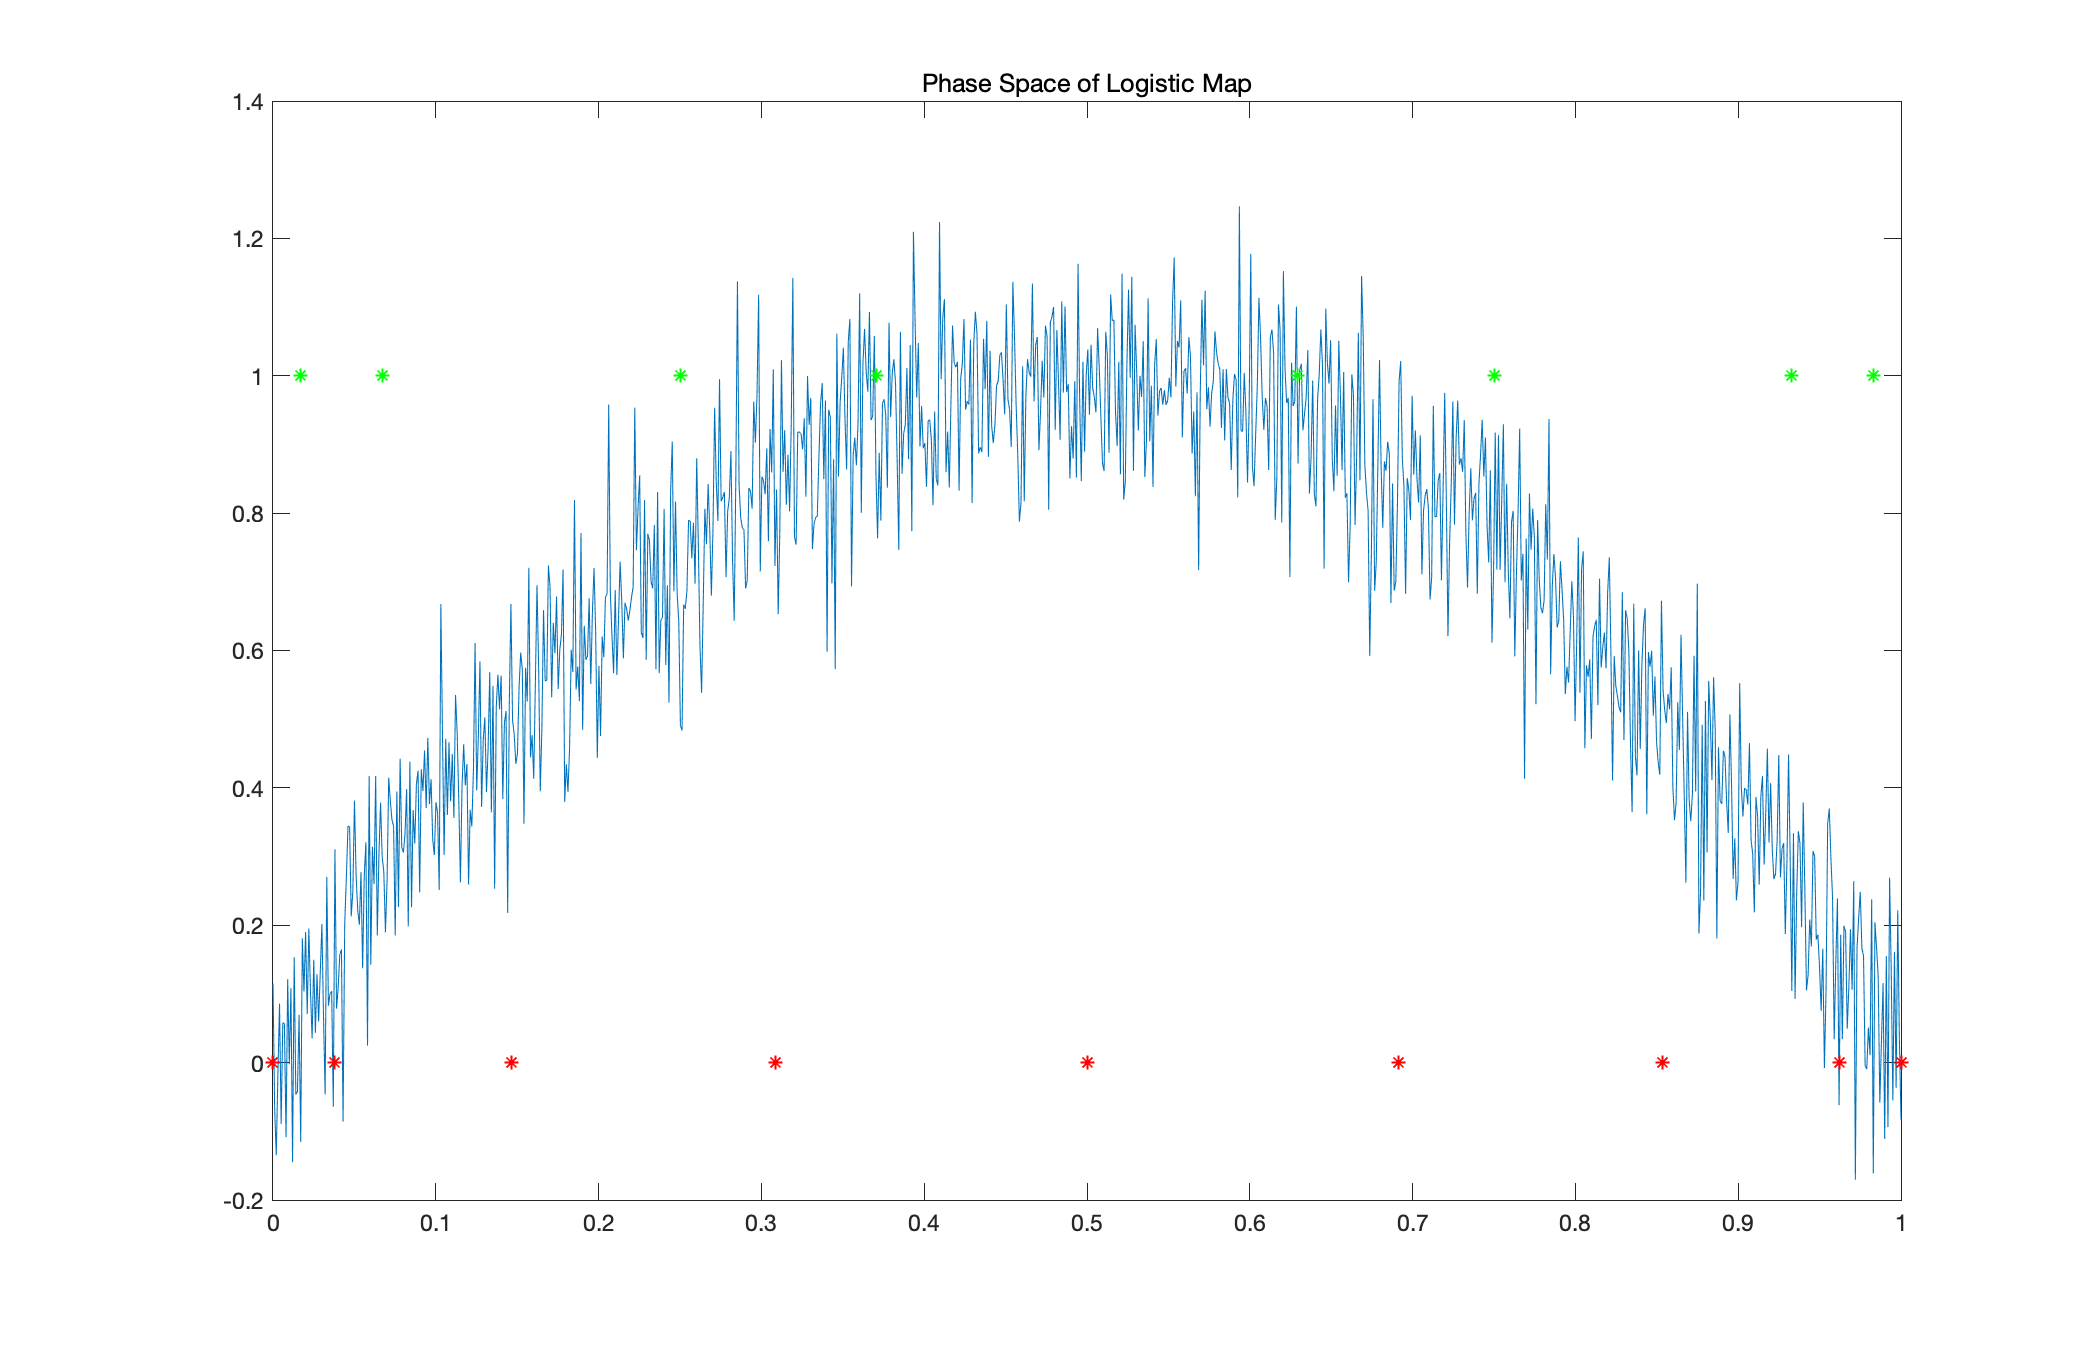
\includegraphics[scale=0.13]{logistic/noise/Logistic_noise_phase_d0-01}}
    \caption[Logistic映射不同噪声下的相空间]{Logistic映射不同噪声下的相空间:noise表示噪声与函数幅值之比}\label{fig:Logistic_noise_phase_d0}
\end{figure}

我们取Logistic映射在$noise=0.001$与$noise=0.01$时Koopman算符对应的本征函数,如图\ref{fig:Logistic_eigen_noise_n1000m20d0-001}与图\ref{fig:Logistic_eigen_noise_n1000m20d0-01}。同样我们在图中标出本征函数极值点的位置,及Logistic边界点的位置,对比图\ref{fig:Logistic_eigen_noise_n1000m2d0}来探究Koopman算符对边界点划分的鲁棒性。同时,我们在计算Koopman算符的矩阵表示时每次从$K$到$L$进行了多次的演化,并取演化的平均值。



\begin{figure}[!]
    \centering%[2,3,4,5,8,10,15,20]
    \subfloat[m=2]{
      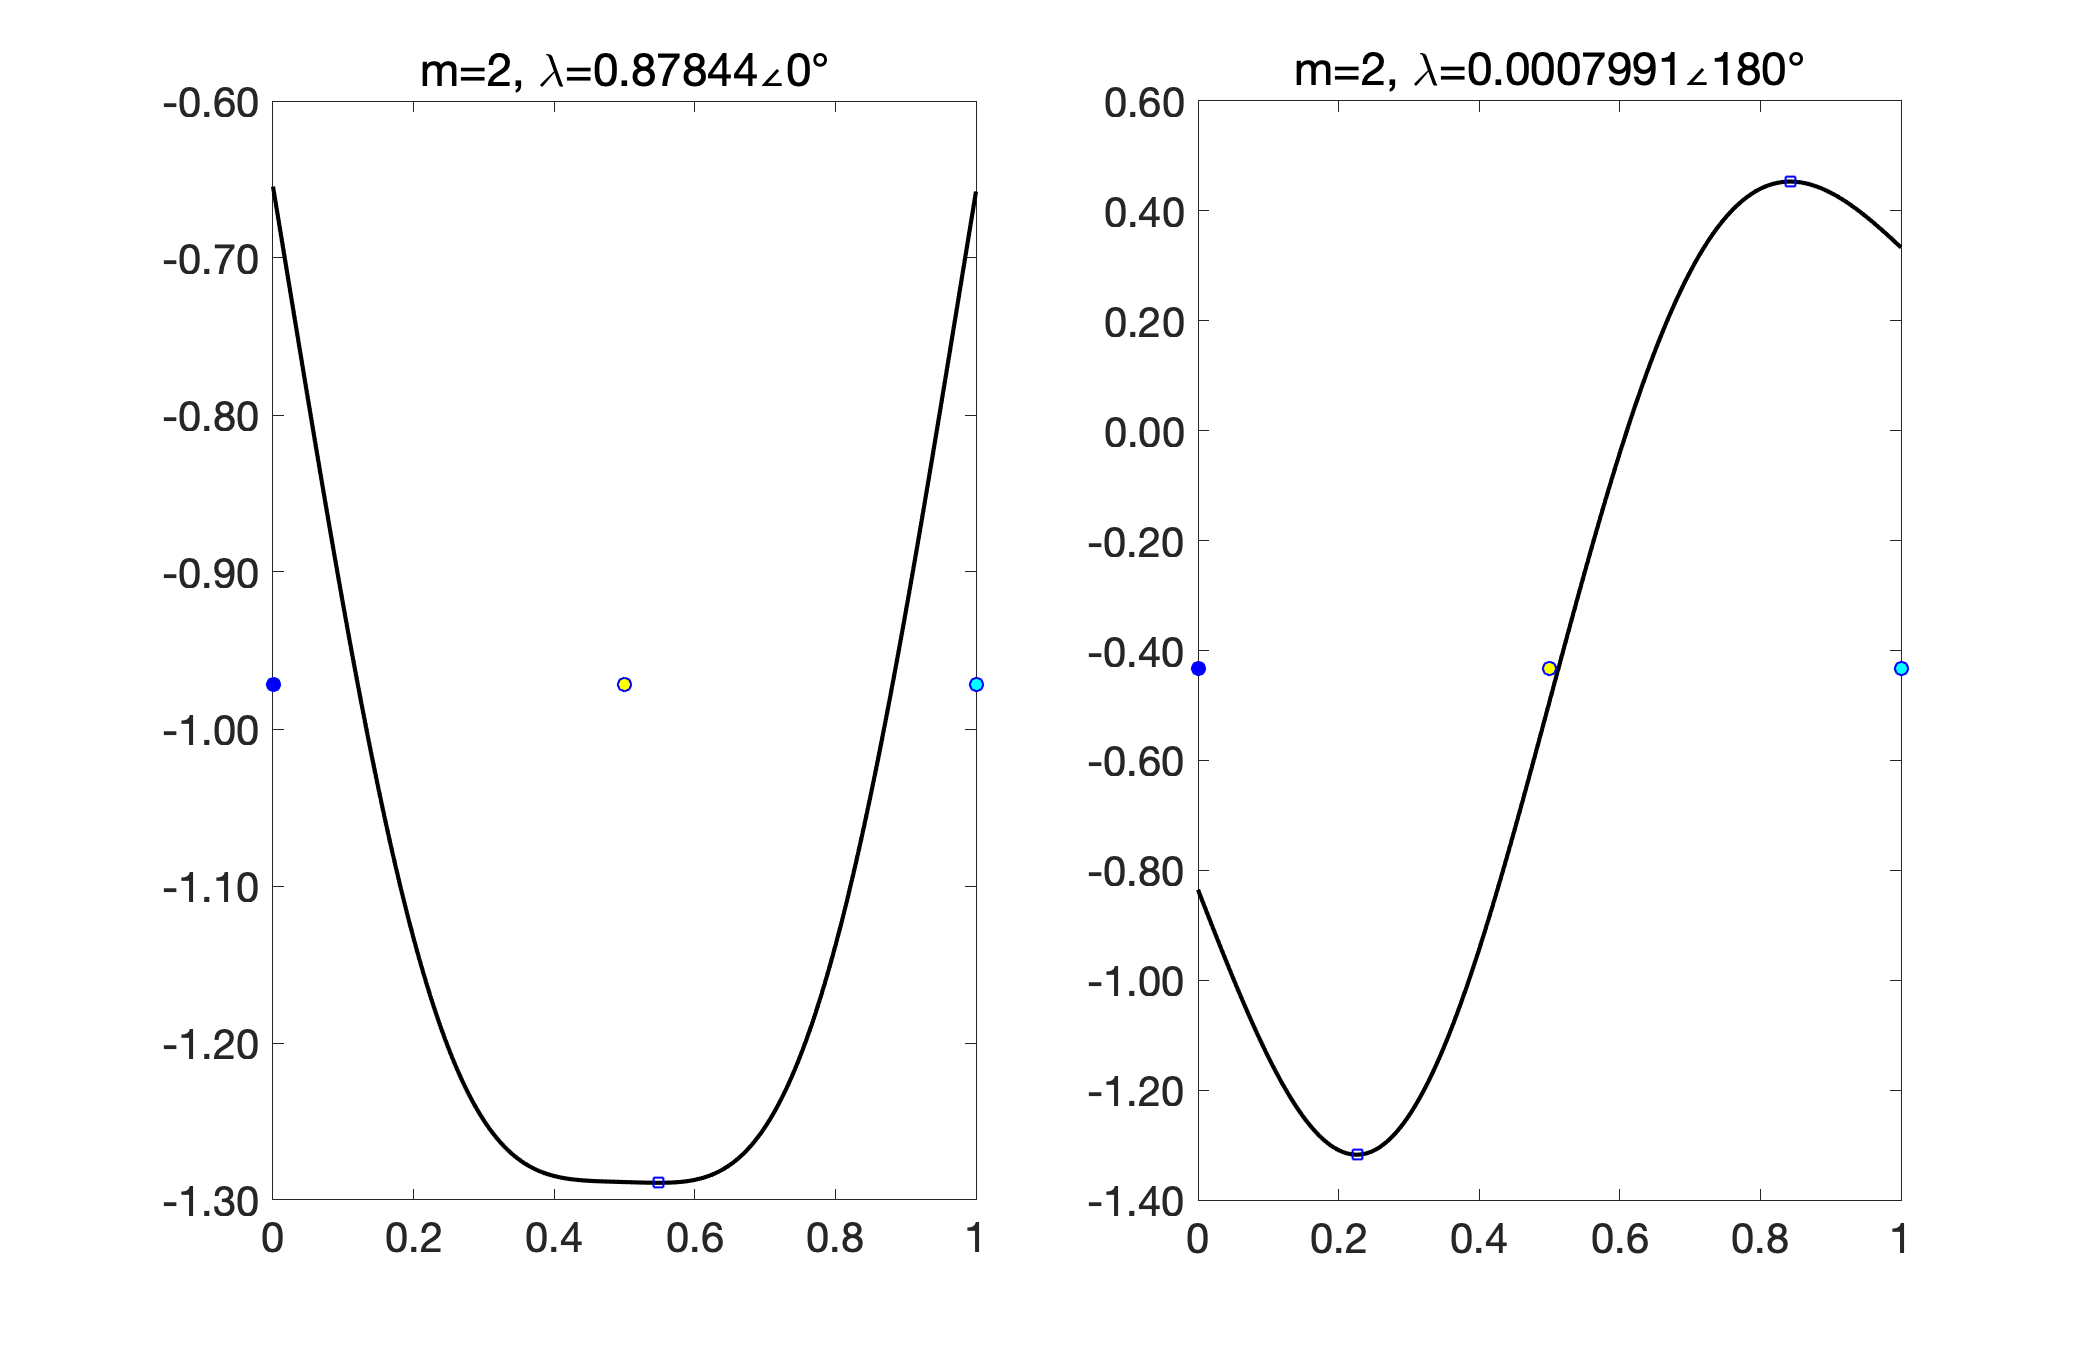
\includegraphics[scale=0.2]{logistic/noise/Logistic_eigen_noise_Gauss_d0-001_n1000_m2}}
    \subfloat[m=3]{
      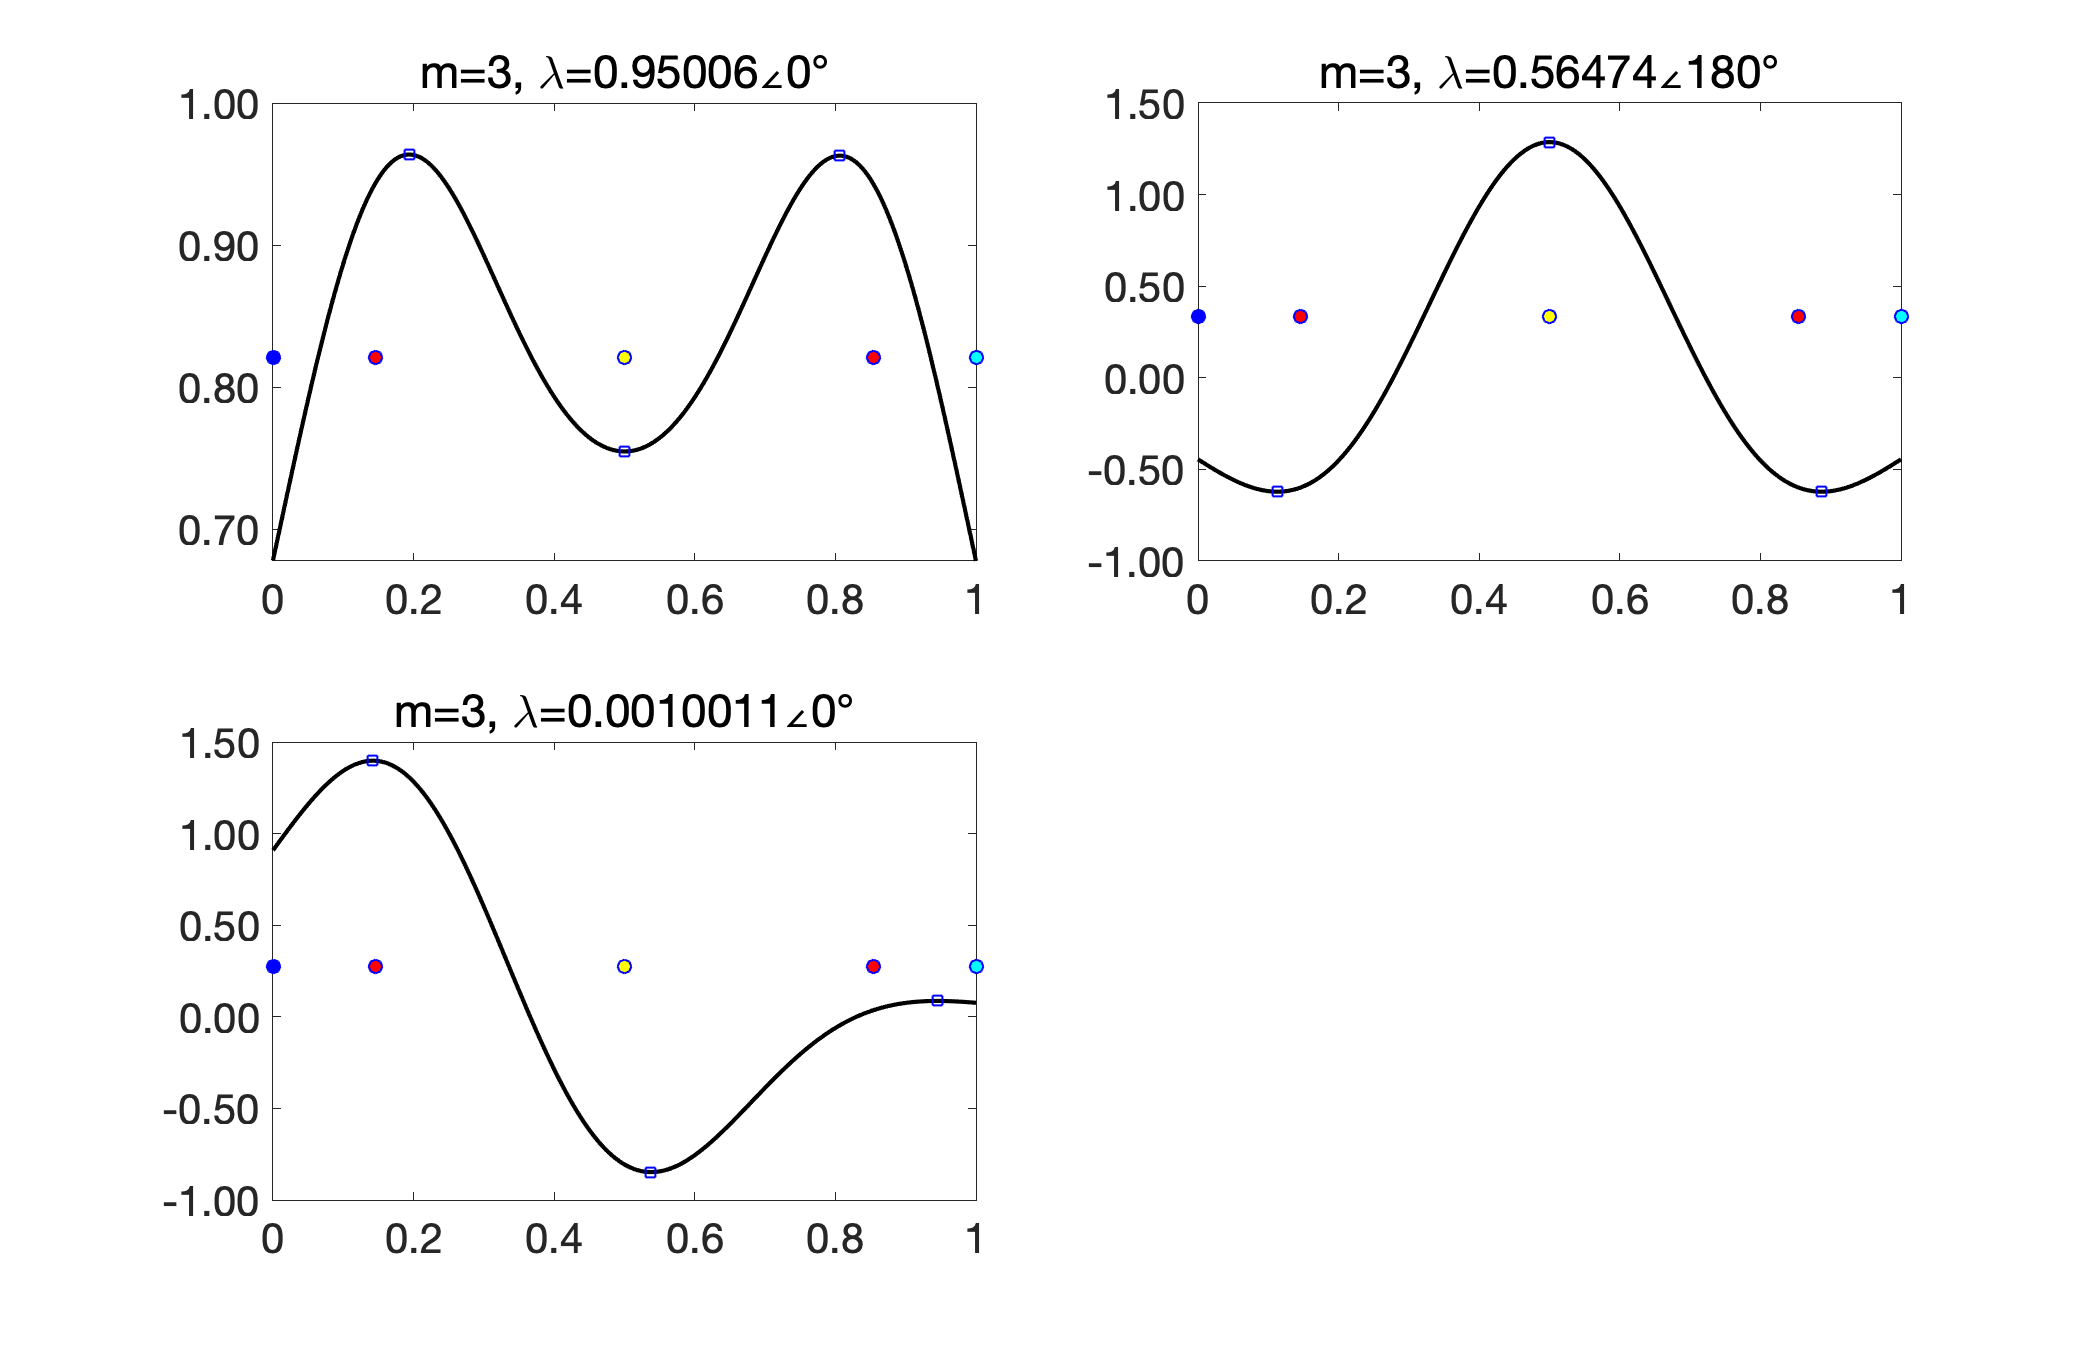
\includegraphics[scale=0.2]{logistic/noise/Logistic_eigen_noise_Gauss_d0-001_n1000_m3}}
      \\
    \subfloat[m=4]{
      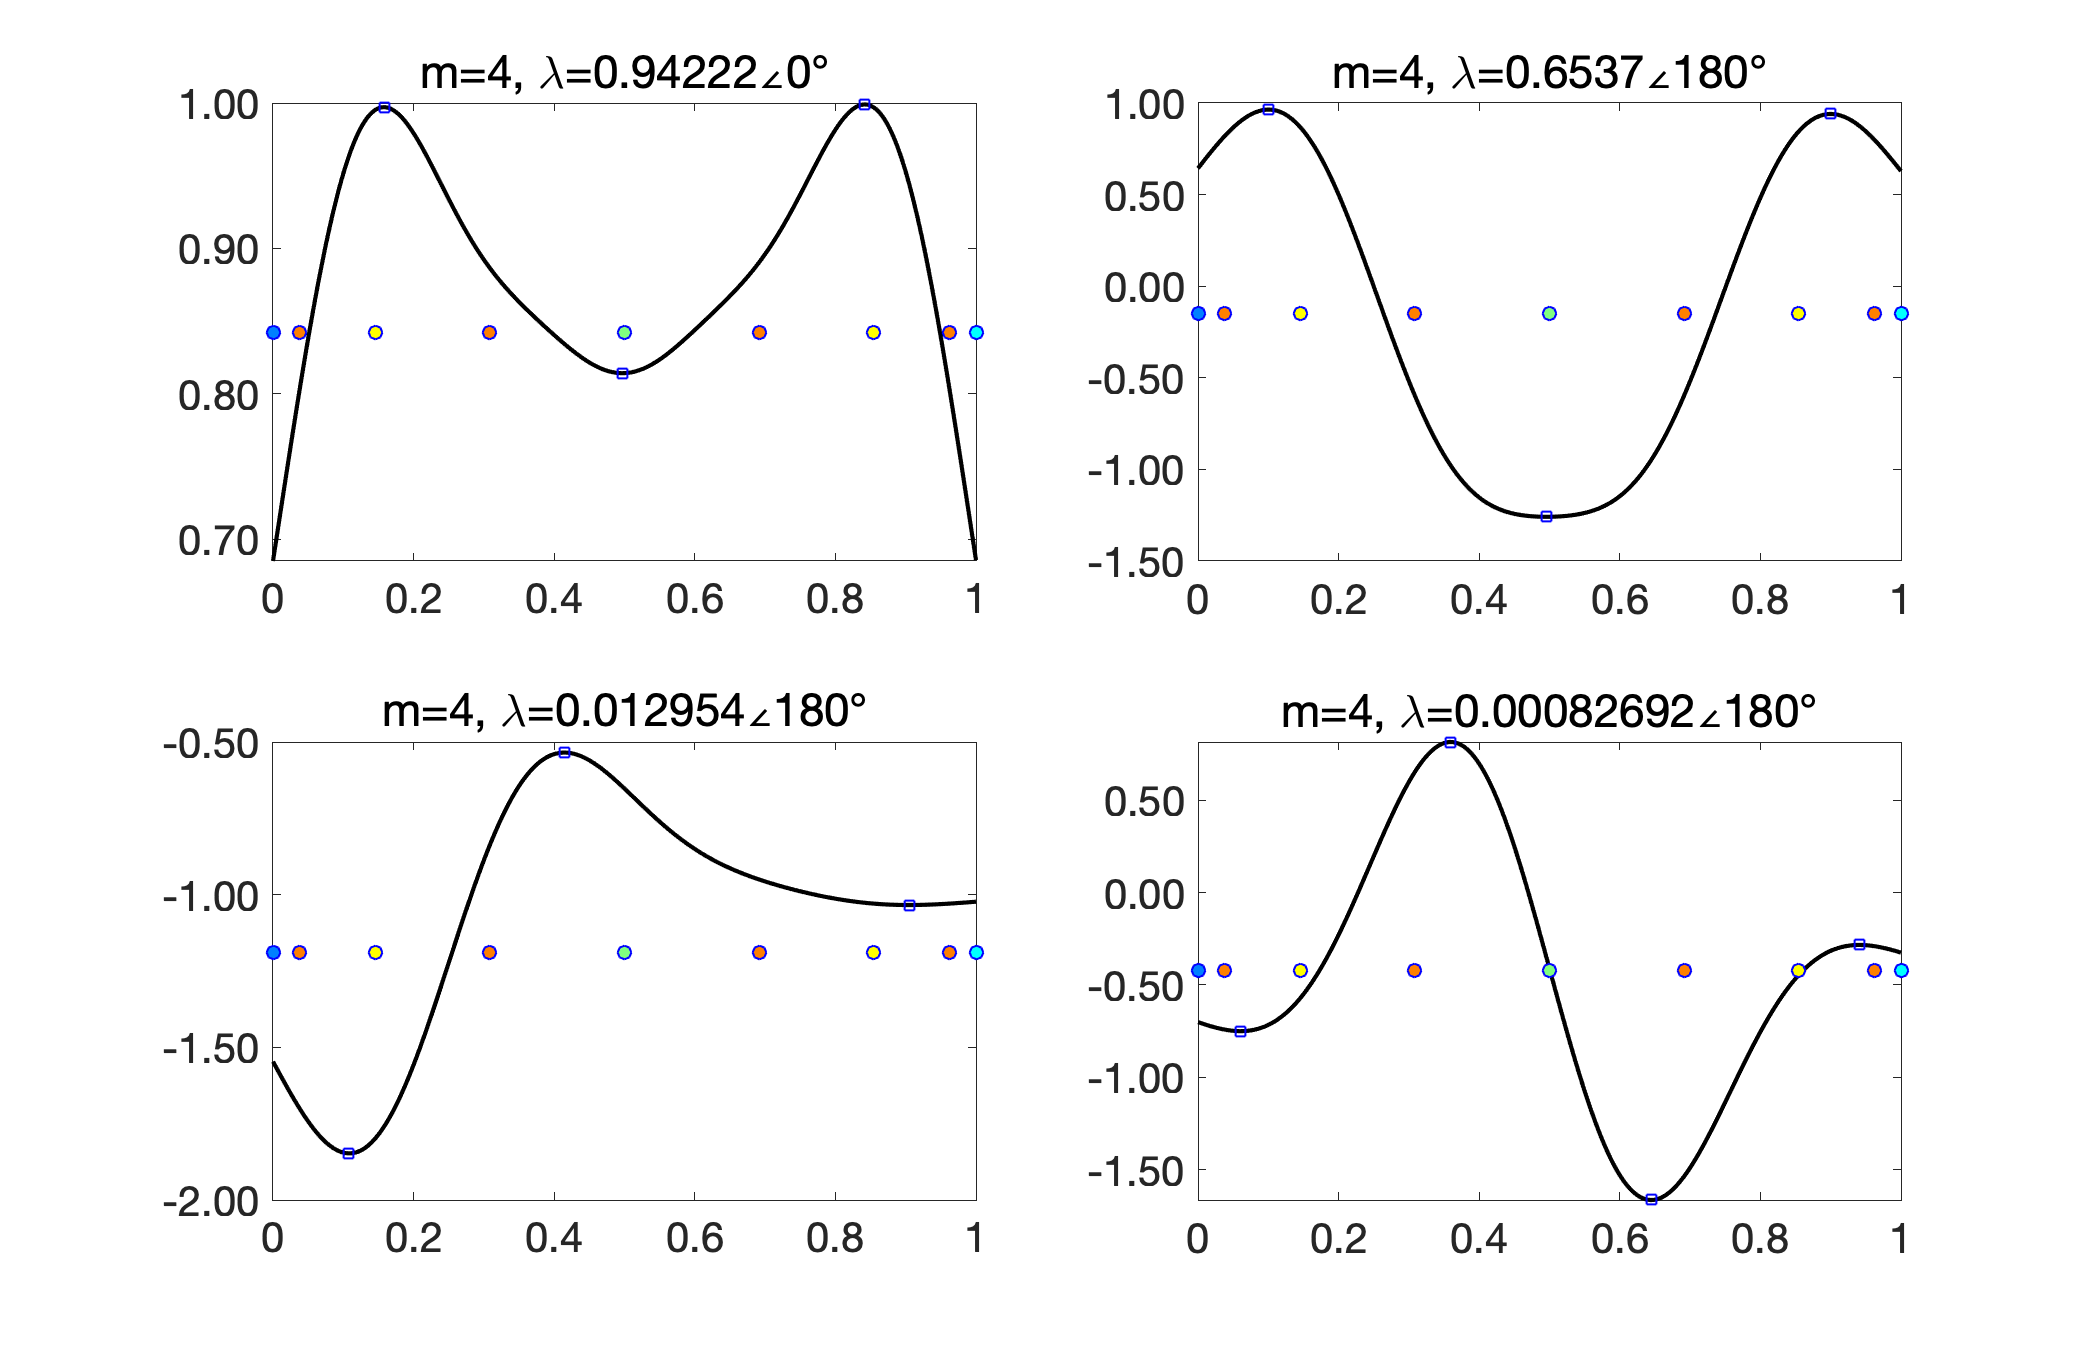
\includegraphics[scale=0.2]{logistic/noise/Logistic_eigen_noise_Gauss_d0-001_n1000_m4}}
    \subfloat[m=5]{
      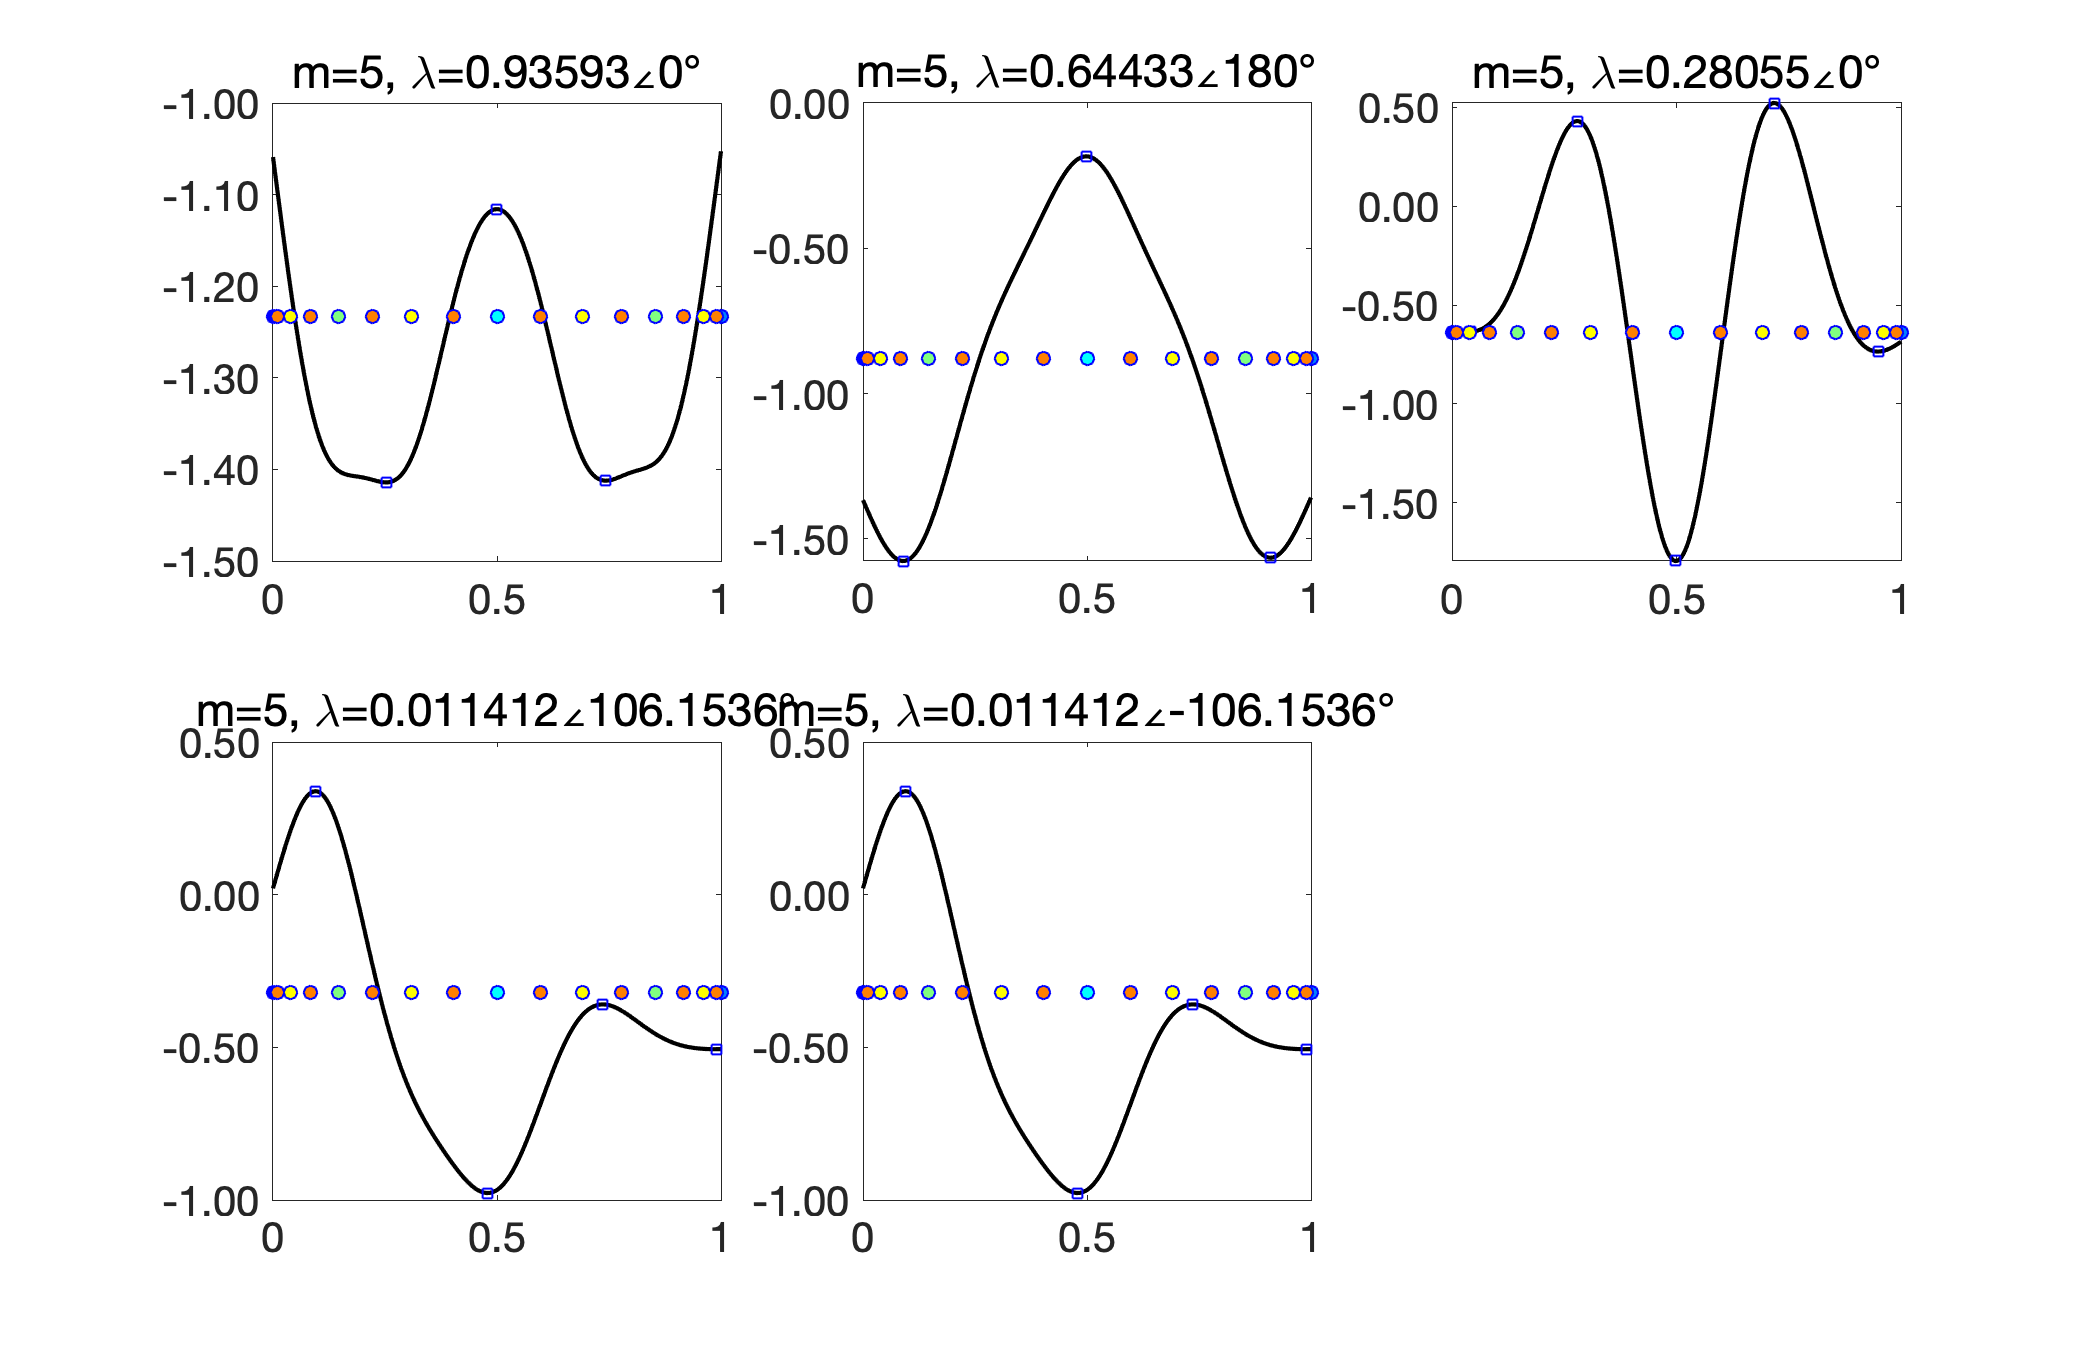
\includegraphics[scale=0.2]{logistic/noise/Logistic_eigen_noise_Gauss_d0-001_n1000_m5}}
      \\
    \subfloat[m=8]{
      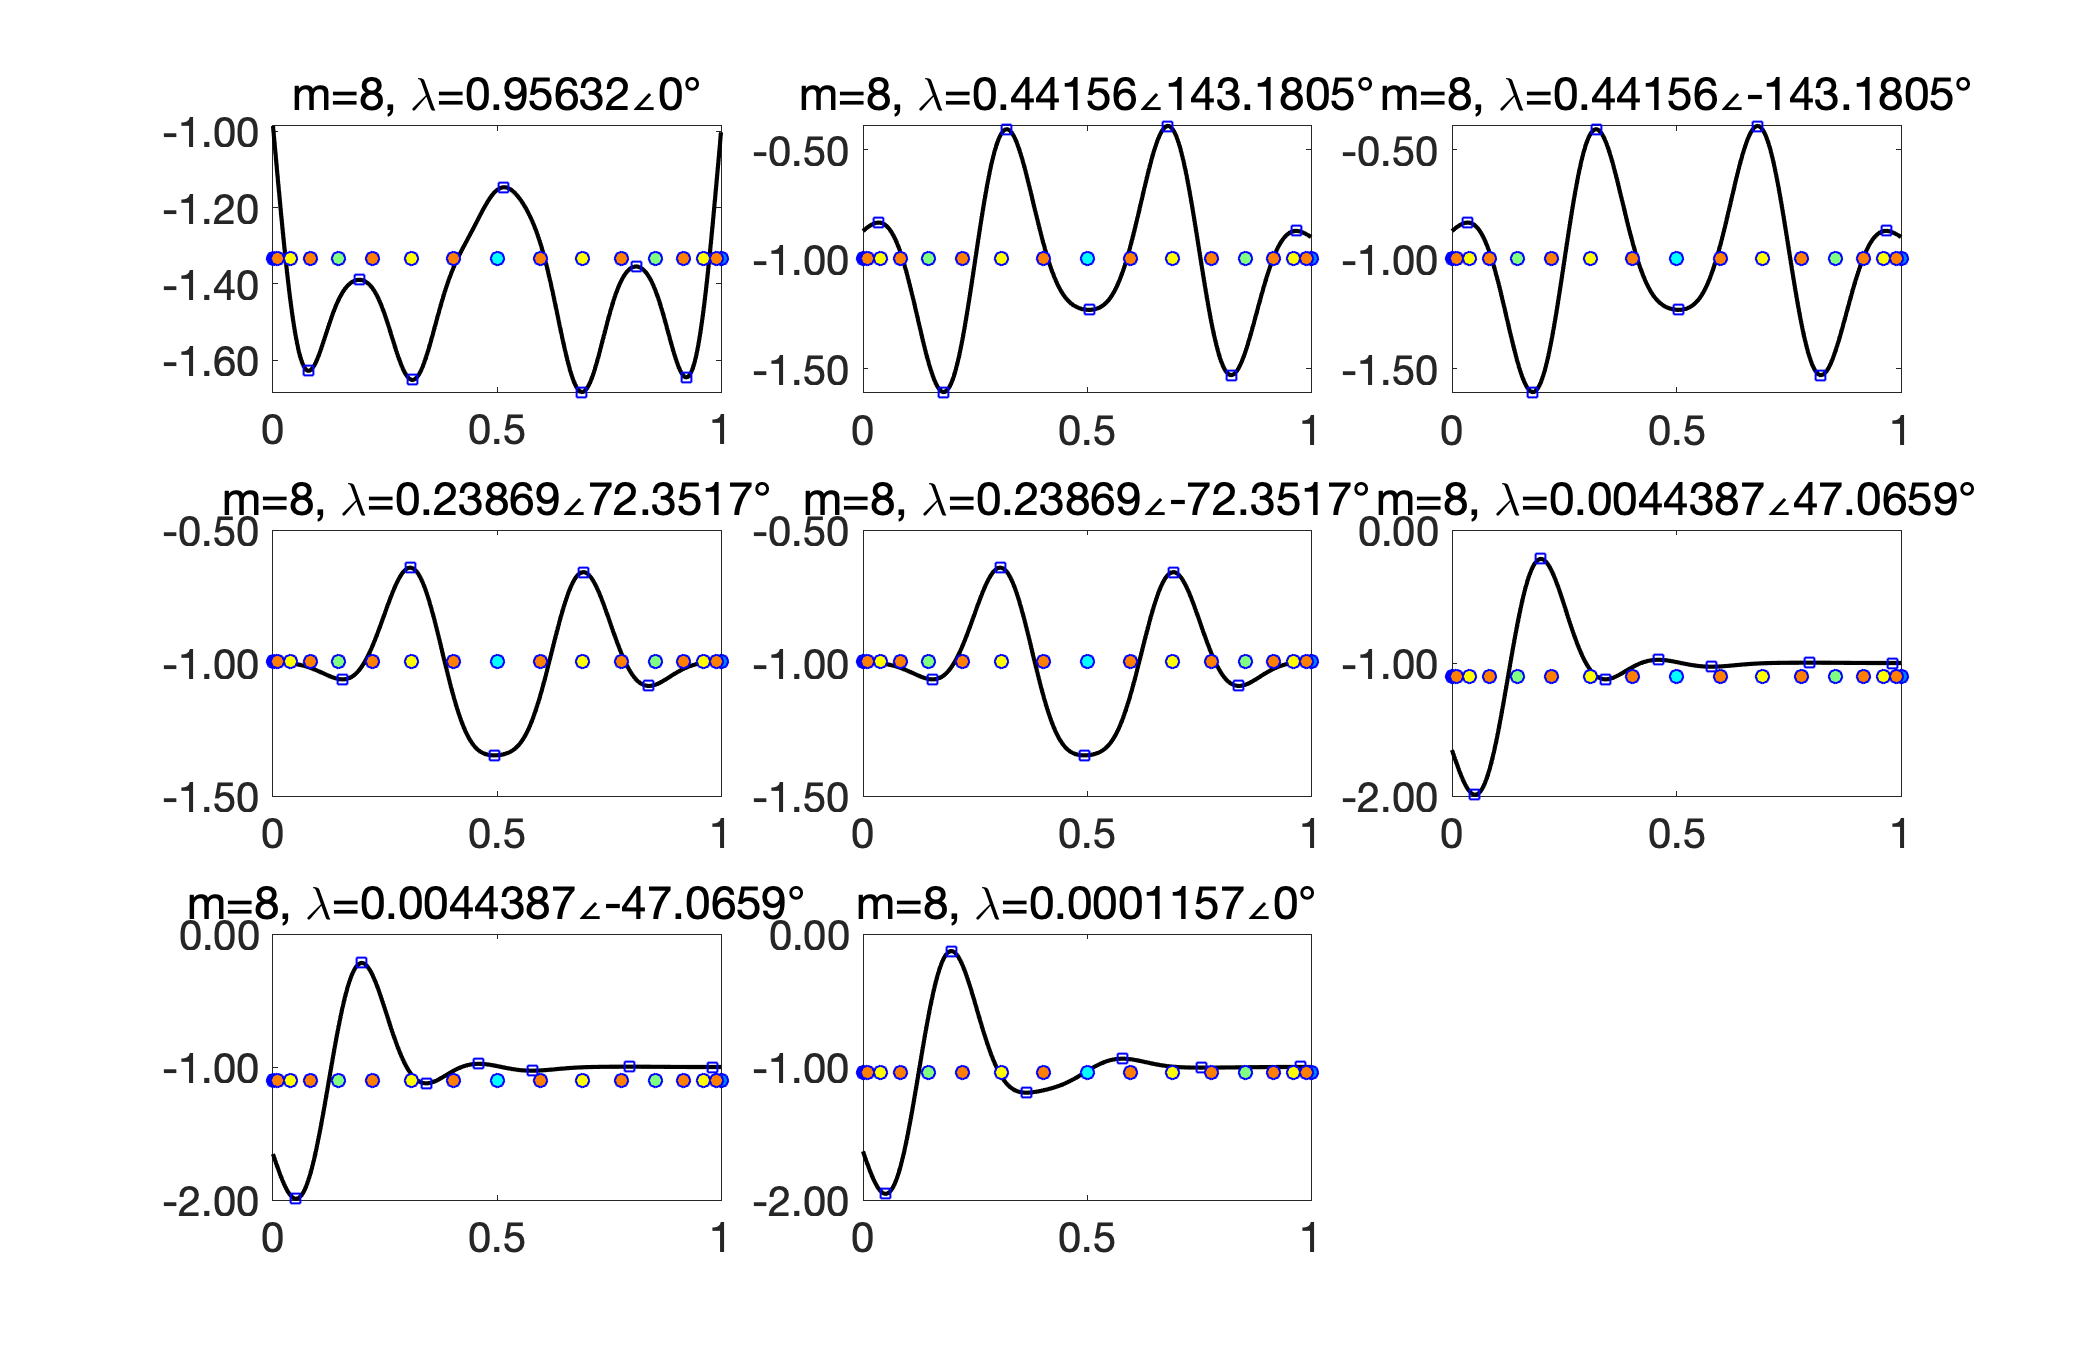
\includegraphics[scale=0.2]{logistic/noise/Logistic_eigen_noise_Gauss_d0-001_n1000_m8}}
    \subfloat[m=10]{
      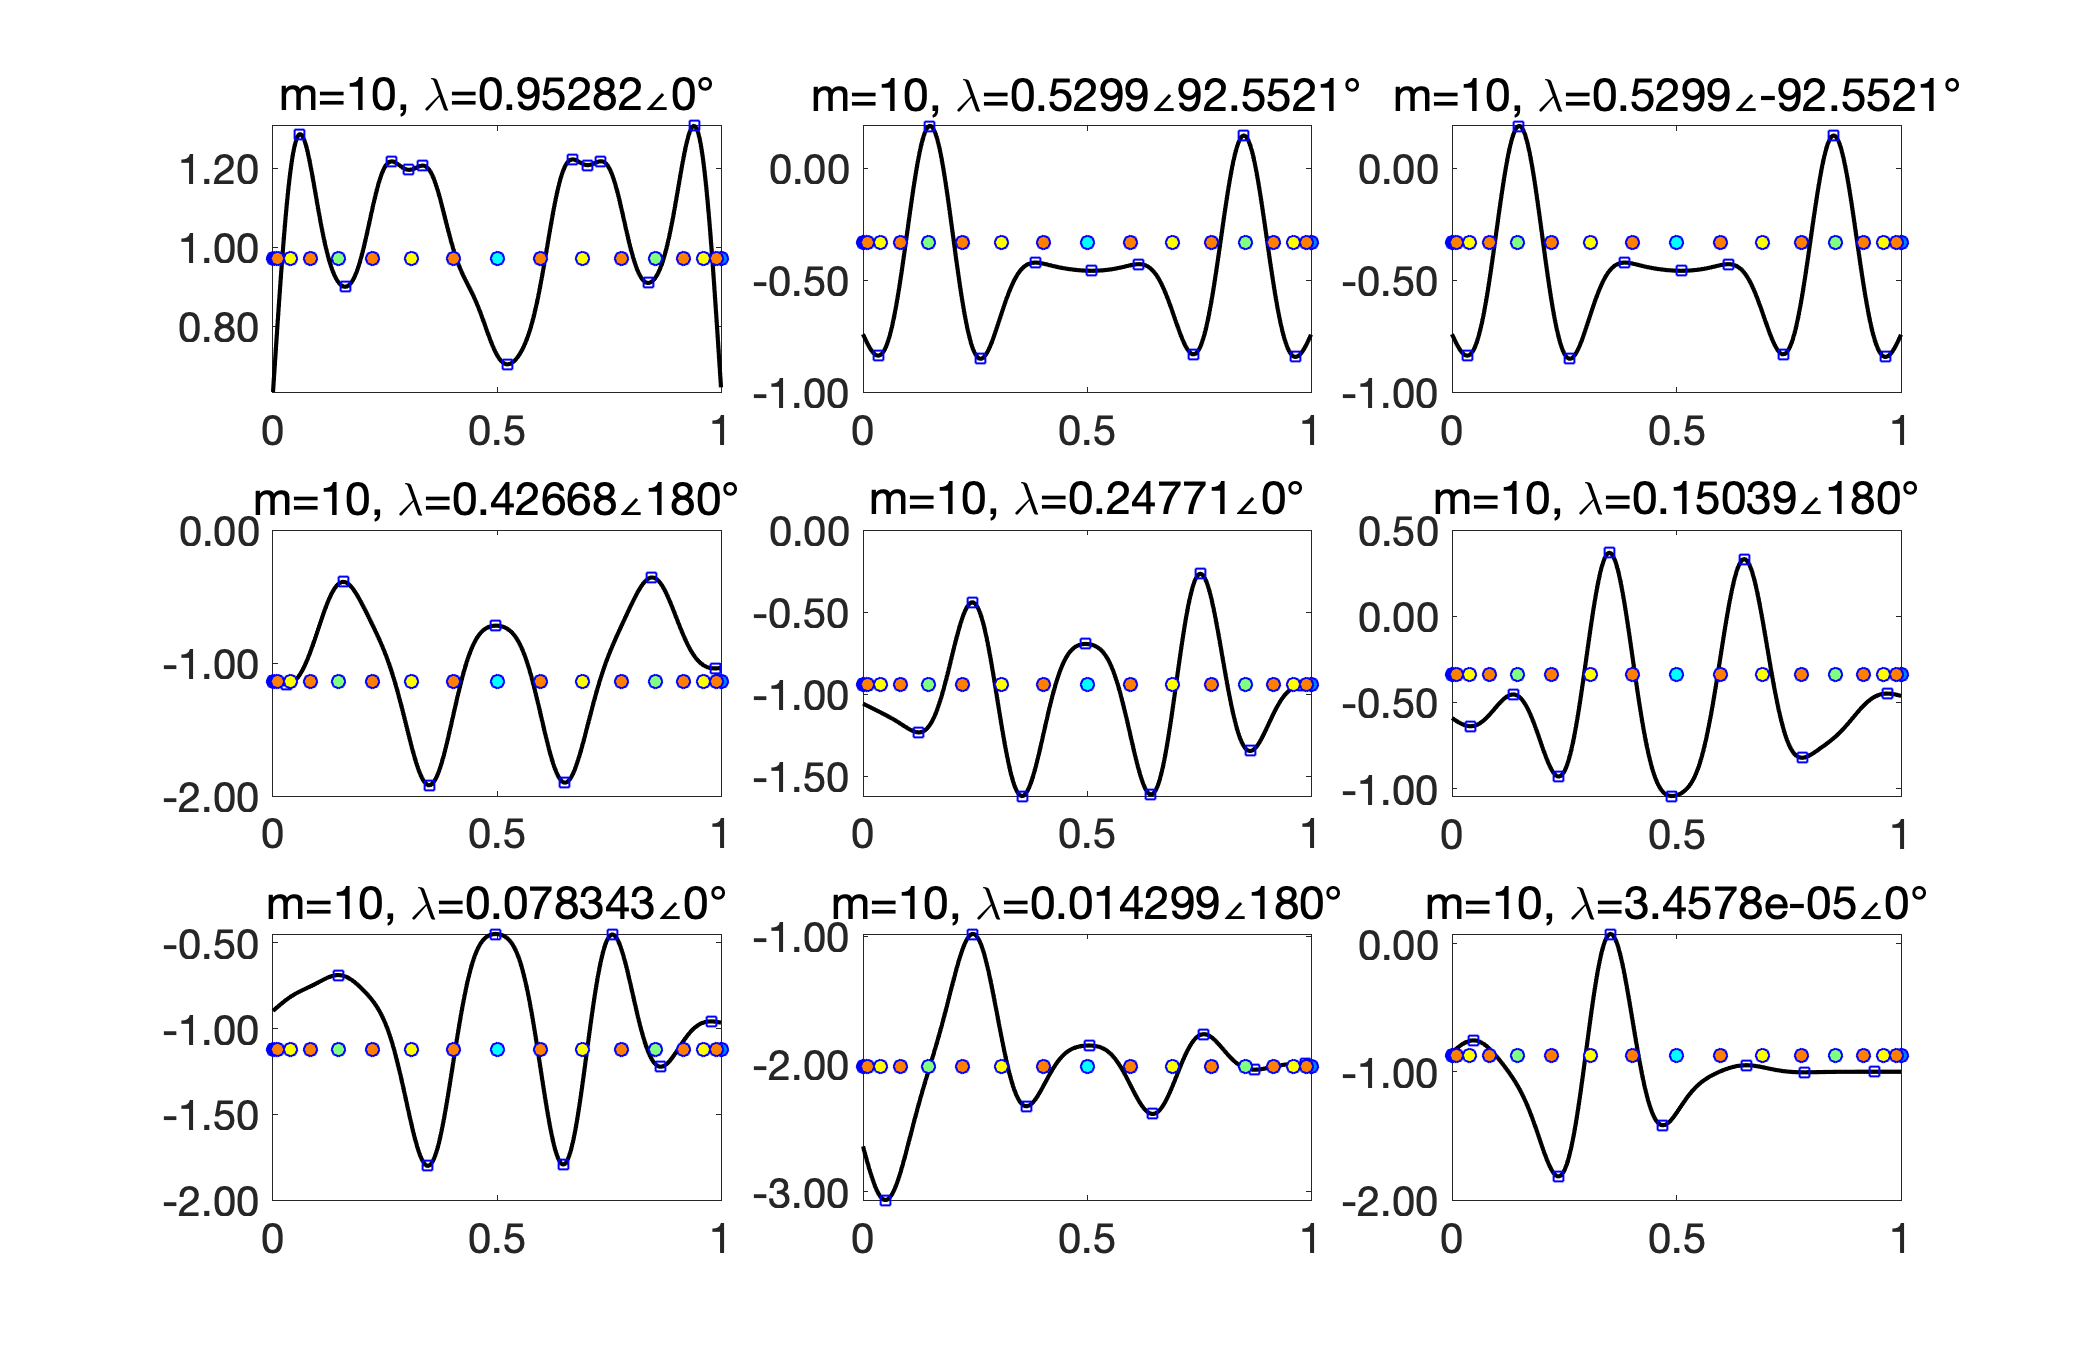
\includegraphics[scale=0.2]{logistic/noise/Logistic_eigen_noise_Gauss_d0-001_n1000_m10}}
      \\
    \subfloat[m=15]{
      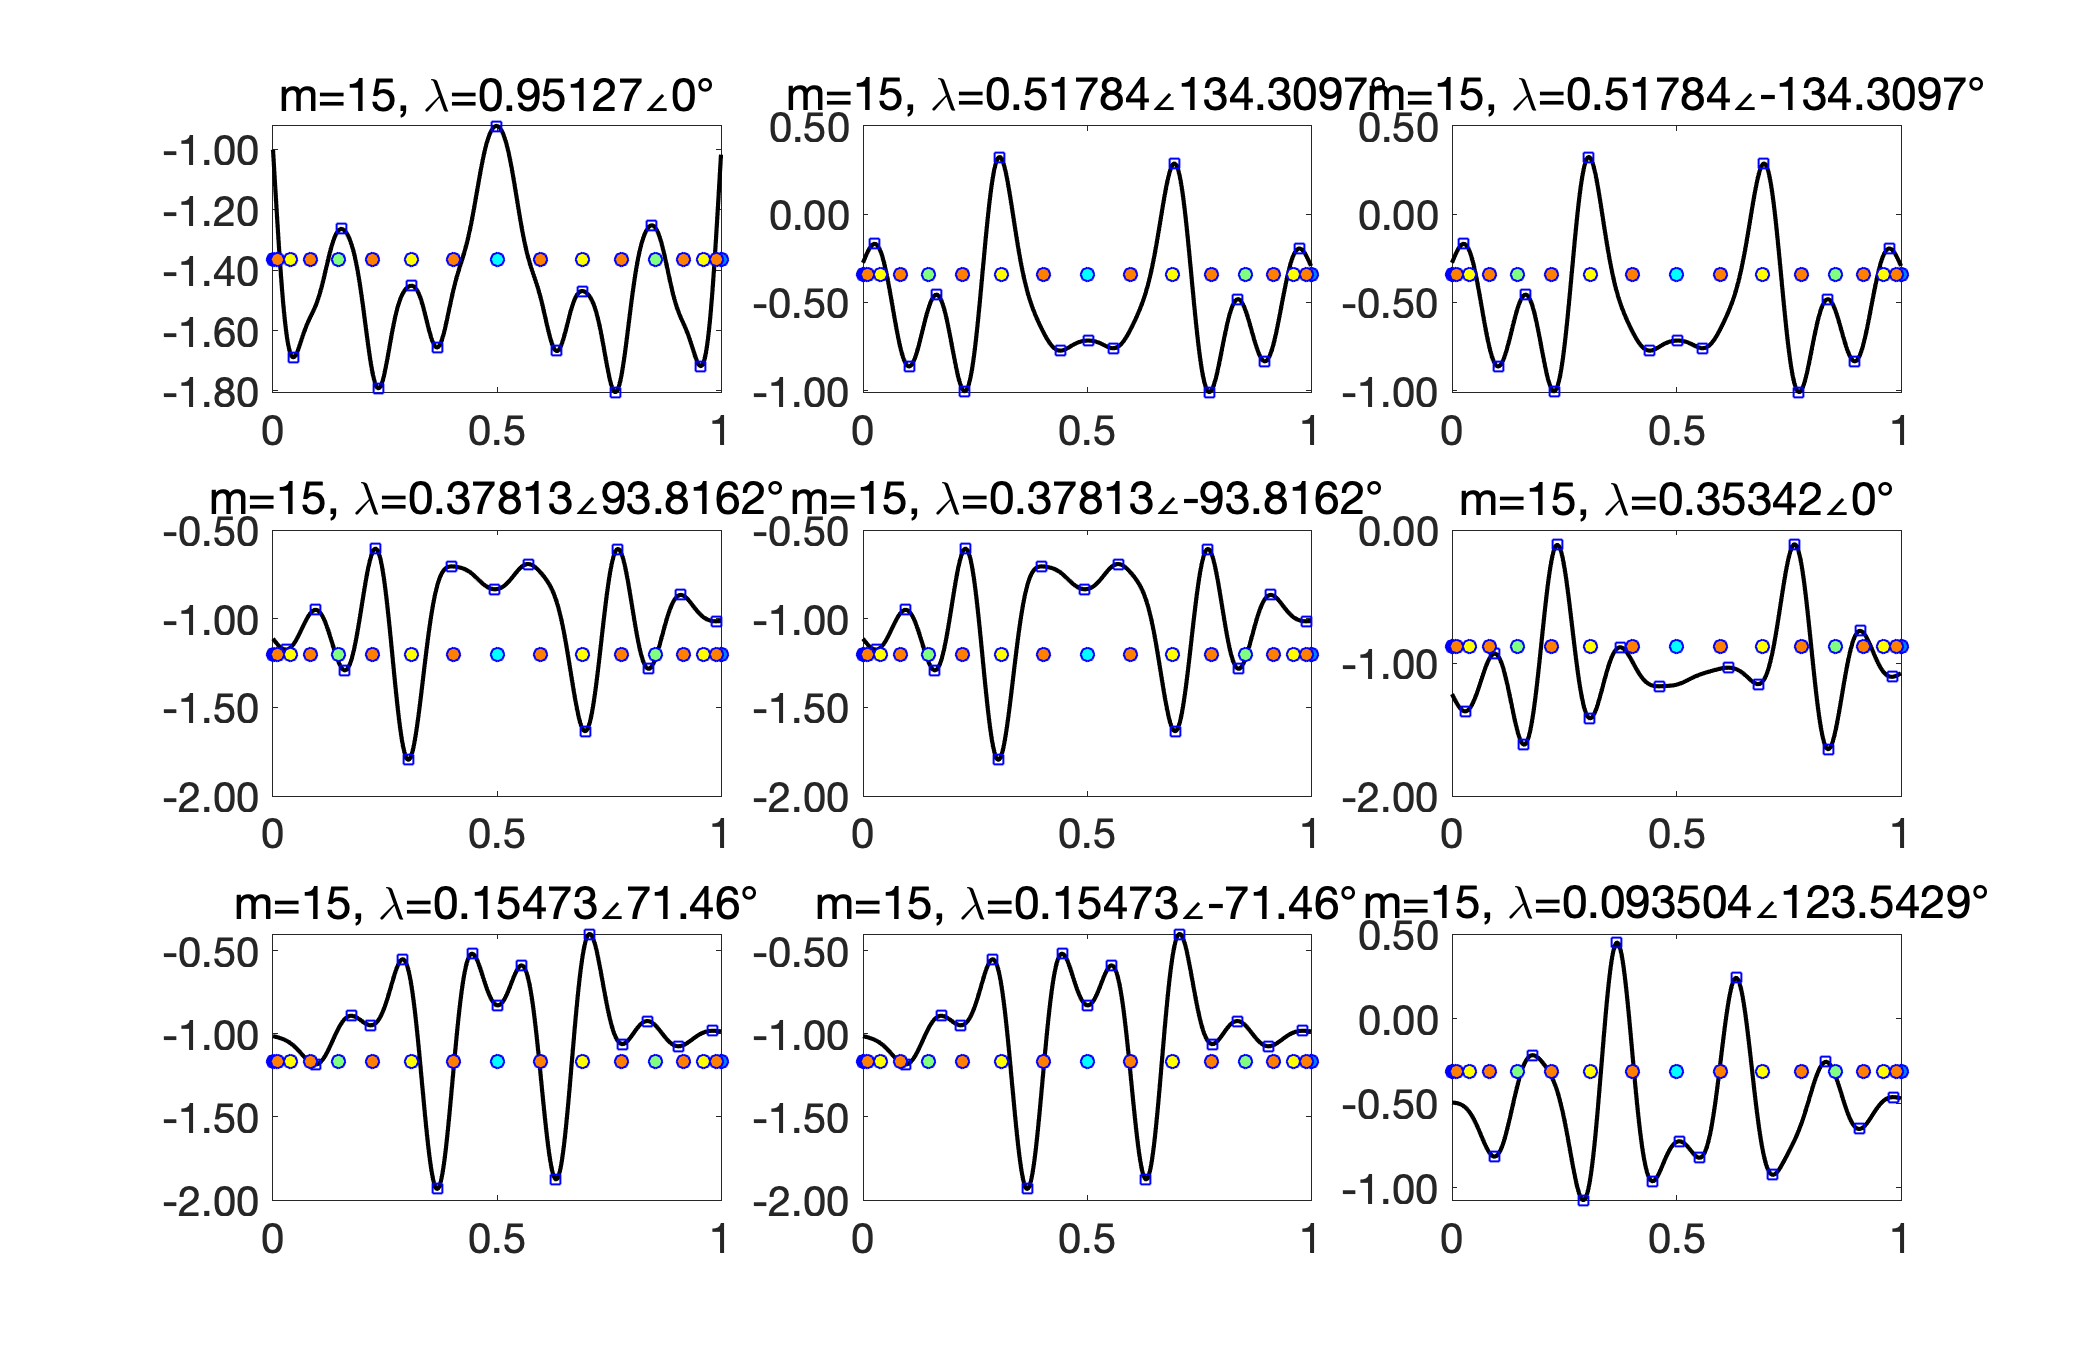
\includegraphics[scale=0.2]{logistic/noise/Logistic_eigen_noise_Gauss_d0-001_n1000_m15}}
    \subfloat[m=20]{
      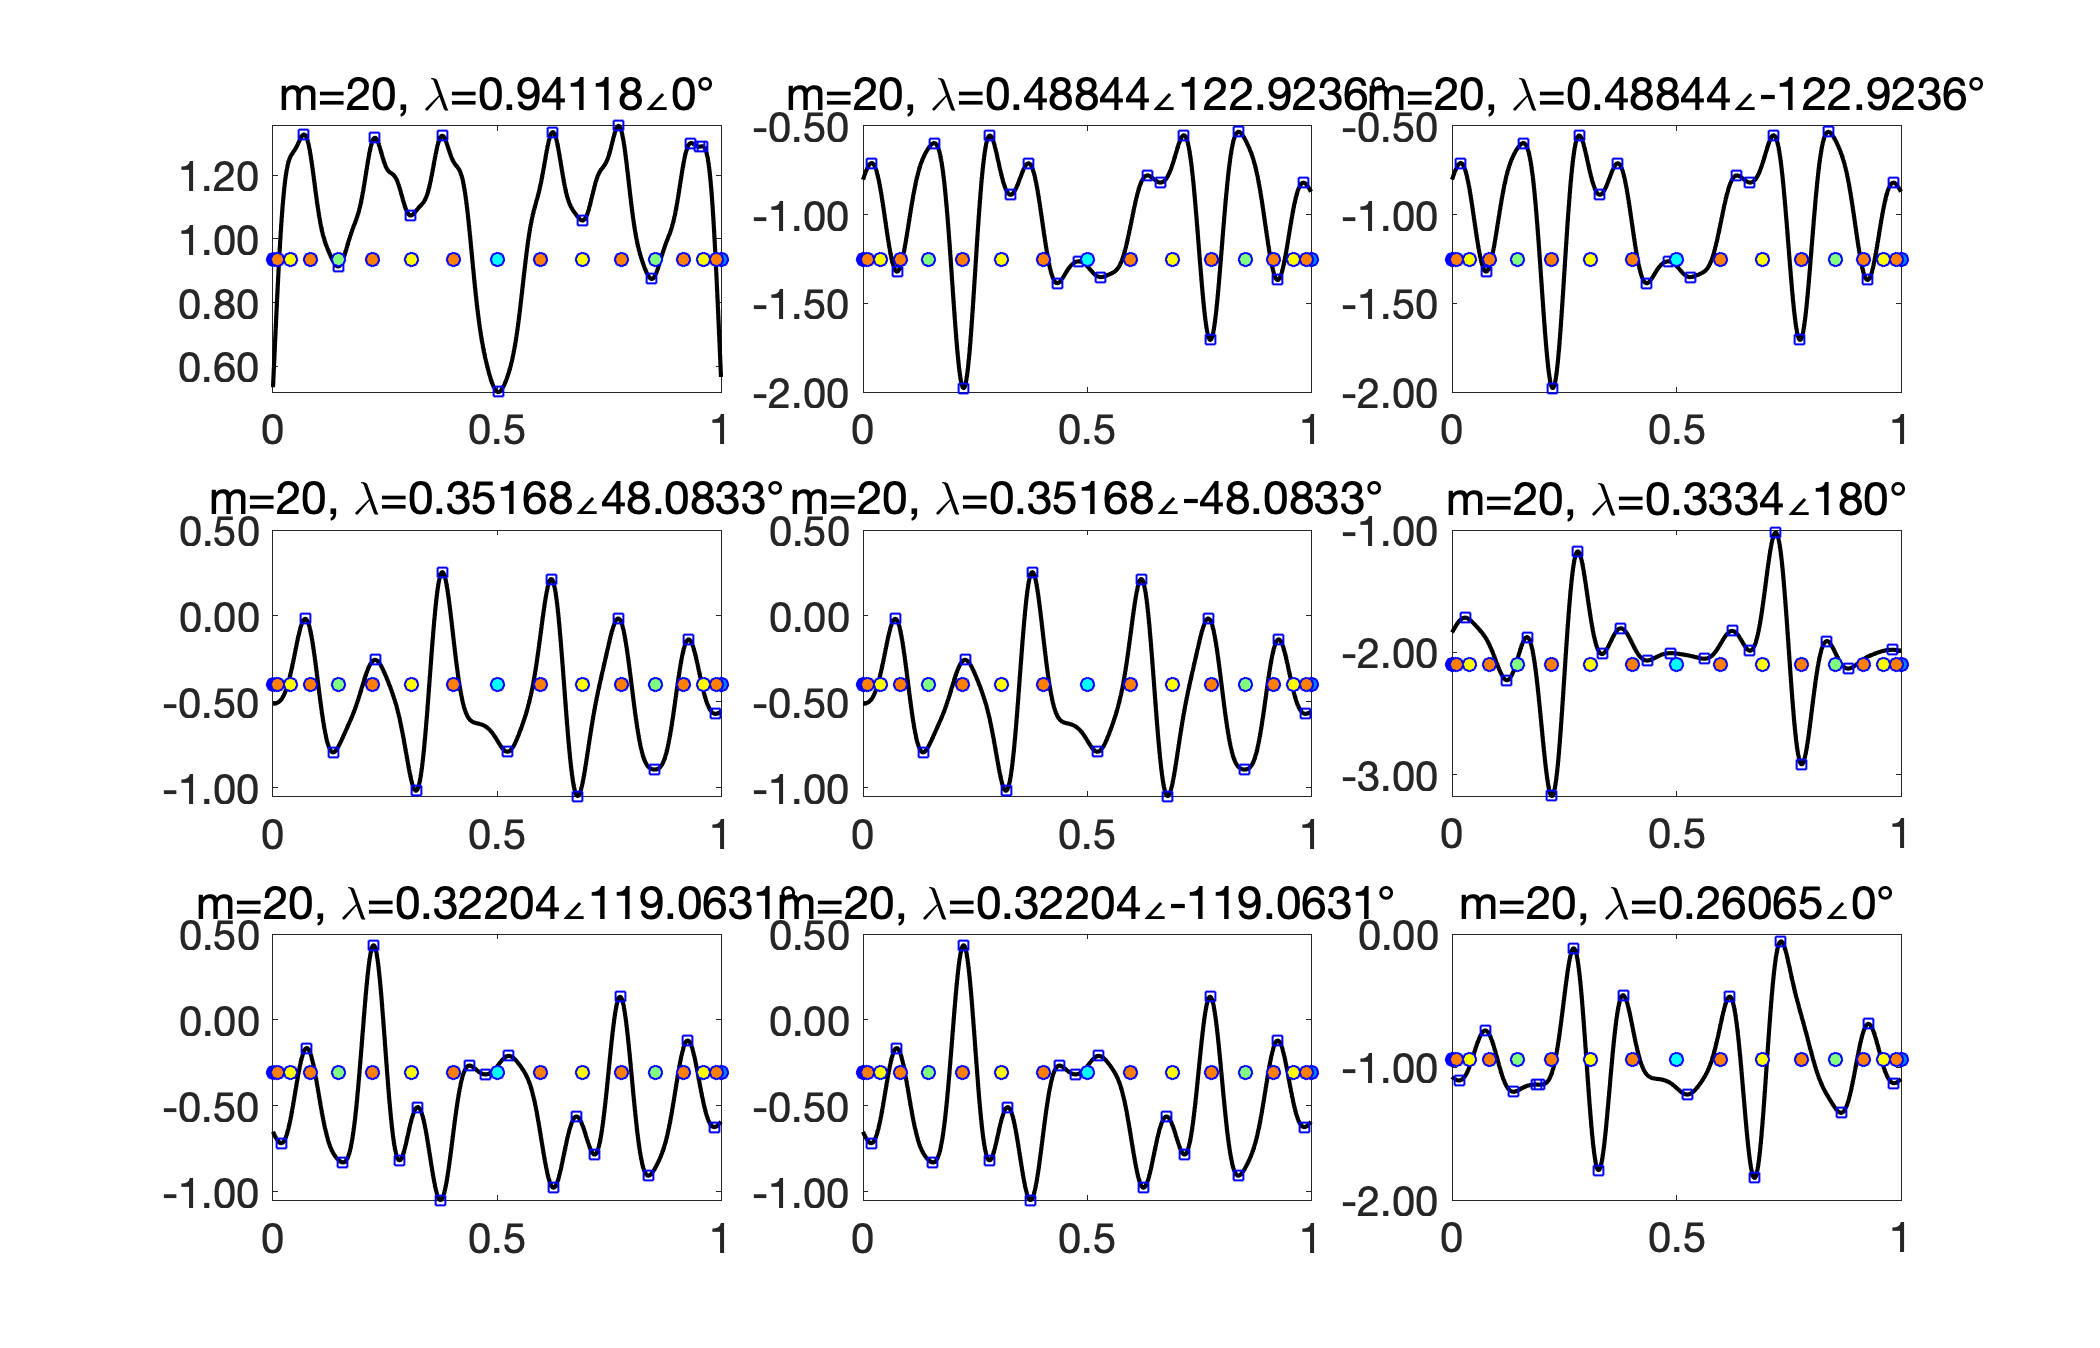
\includegraphics[scale=0.2]{logistic/noise/Logistic_eigen_noise_Gauss_d0-001_n1000_m20}}
      \\
    \caption{Logistic射的边界点与本征函数($noise=0.001$)}\label{fig:Logistic_eigen_noise_n1000m20d0-001}
\end{figure}
  
\begin{figure}[!]
    \centering%[2,3,4,5,8,10,15,20]
    \subfloat[m=2]{
      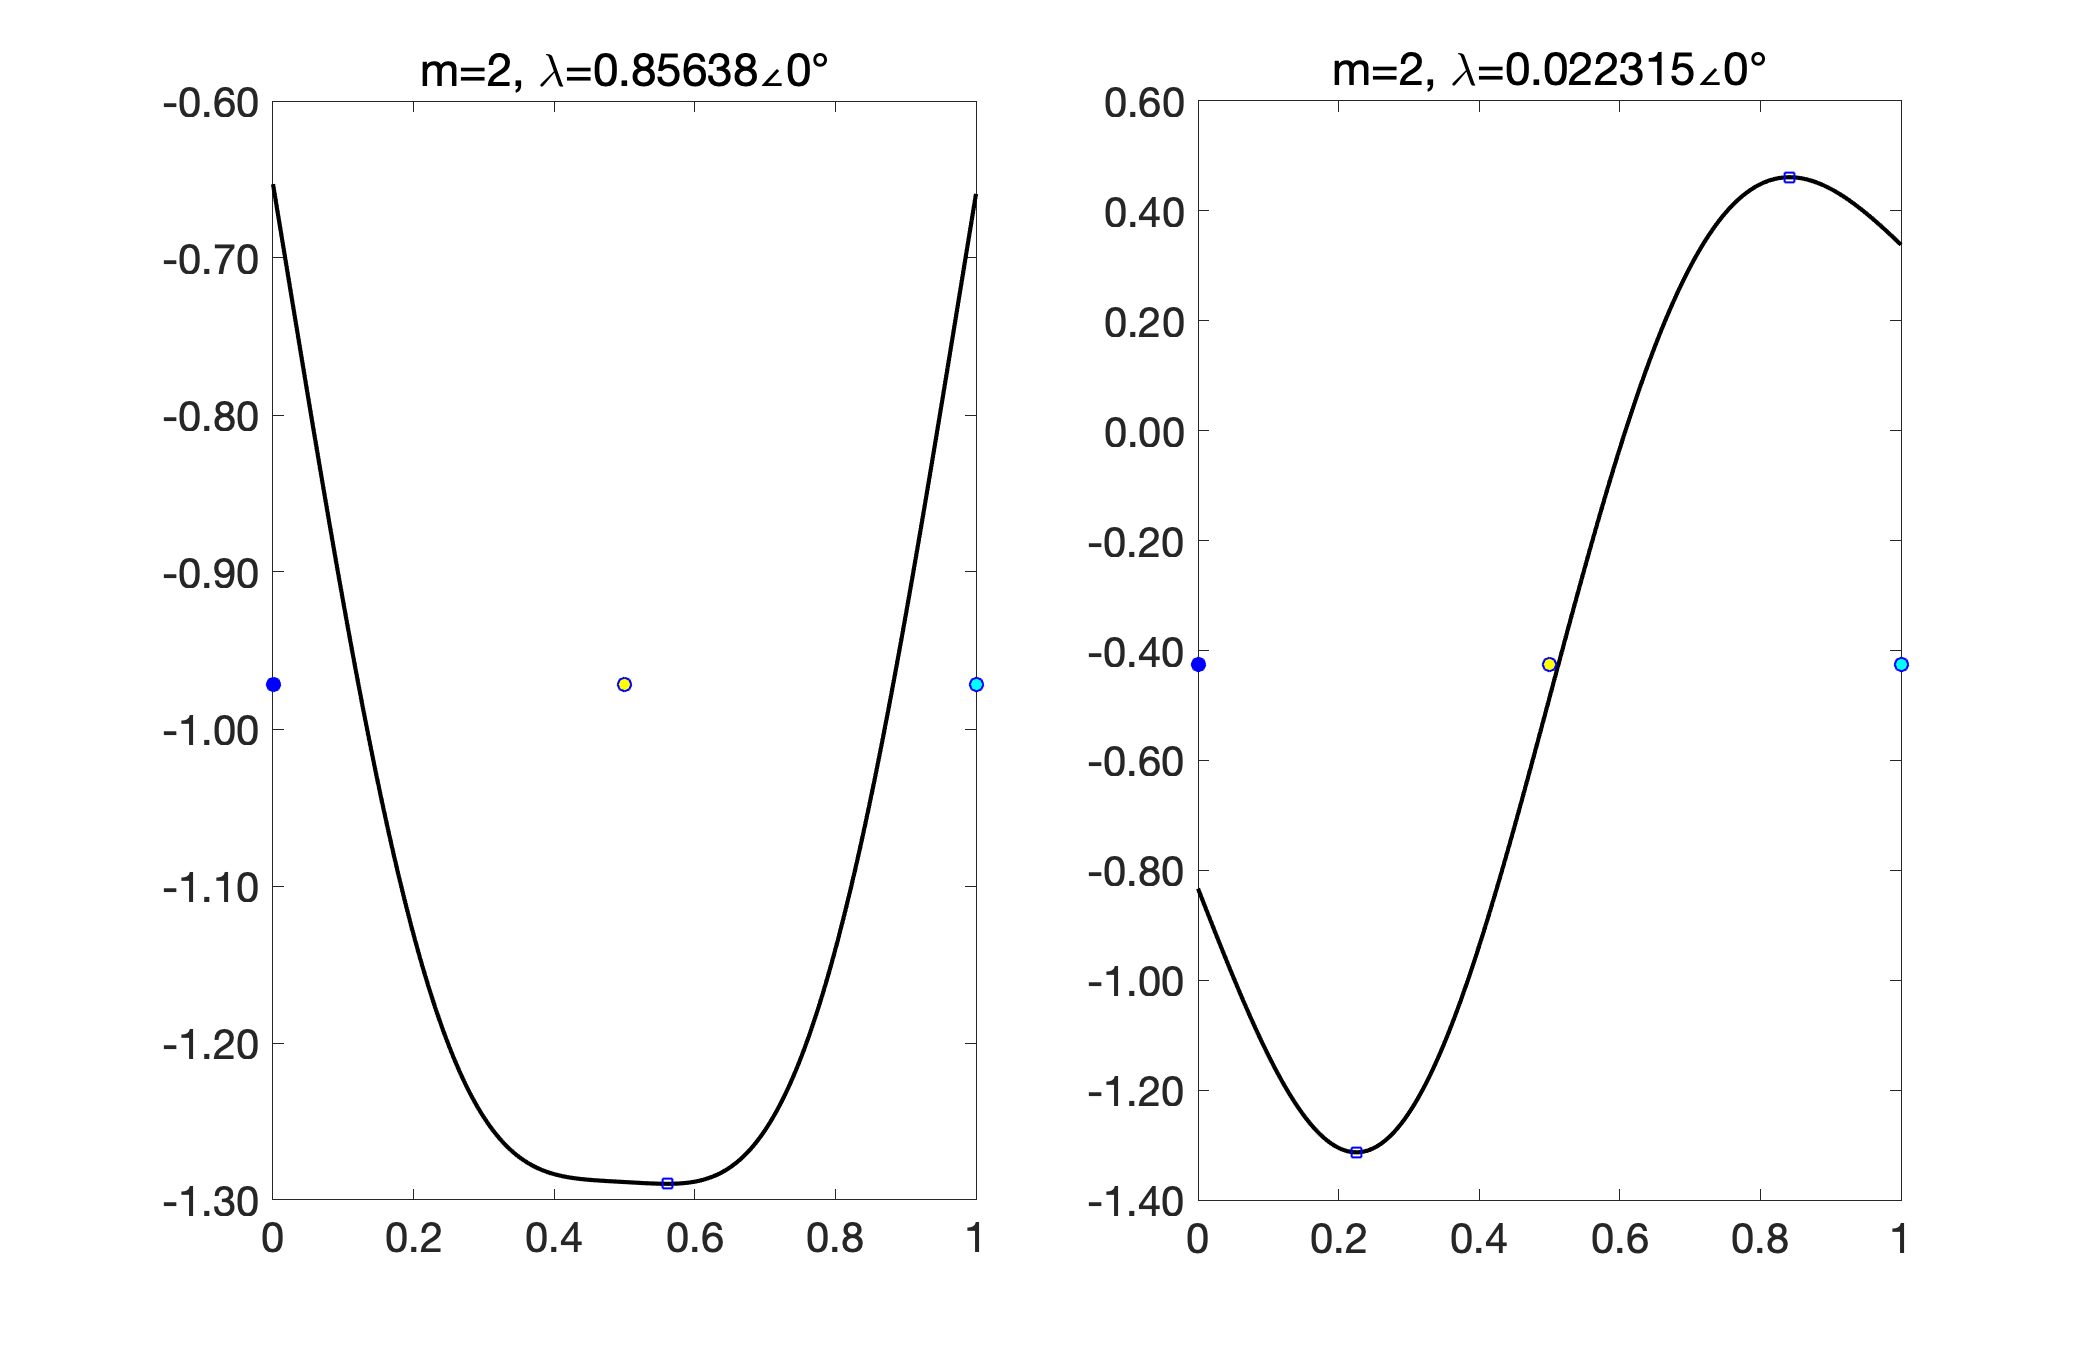
\includegraphics[scale=0.2]{logistic/noise/Logistic_eigen_noise_Gauss_d0-01_n1000_m2}}
    \subfloat[m=3]{
      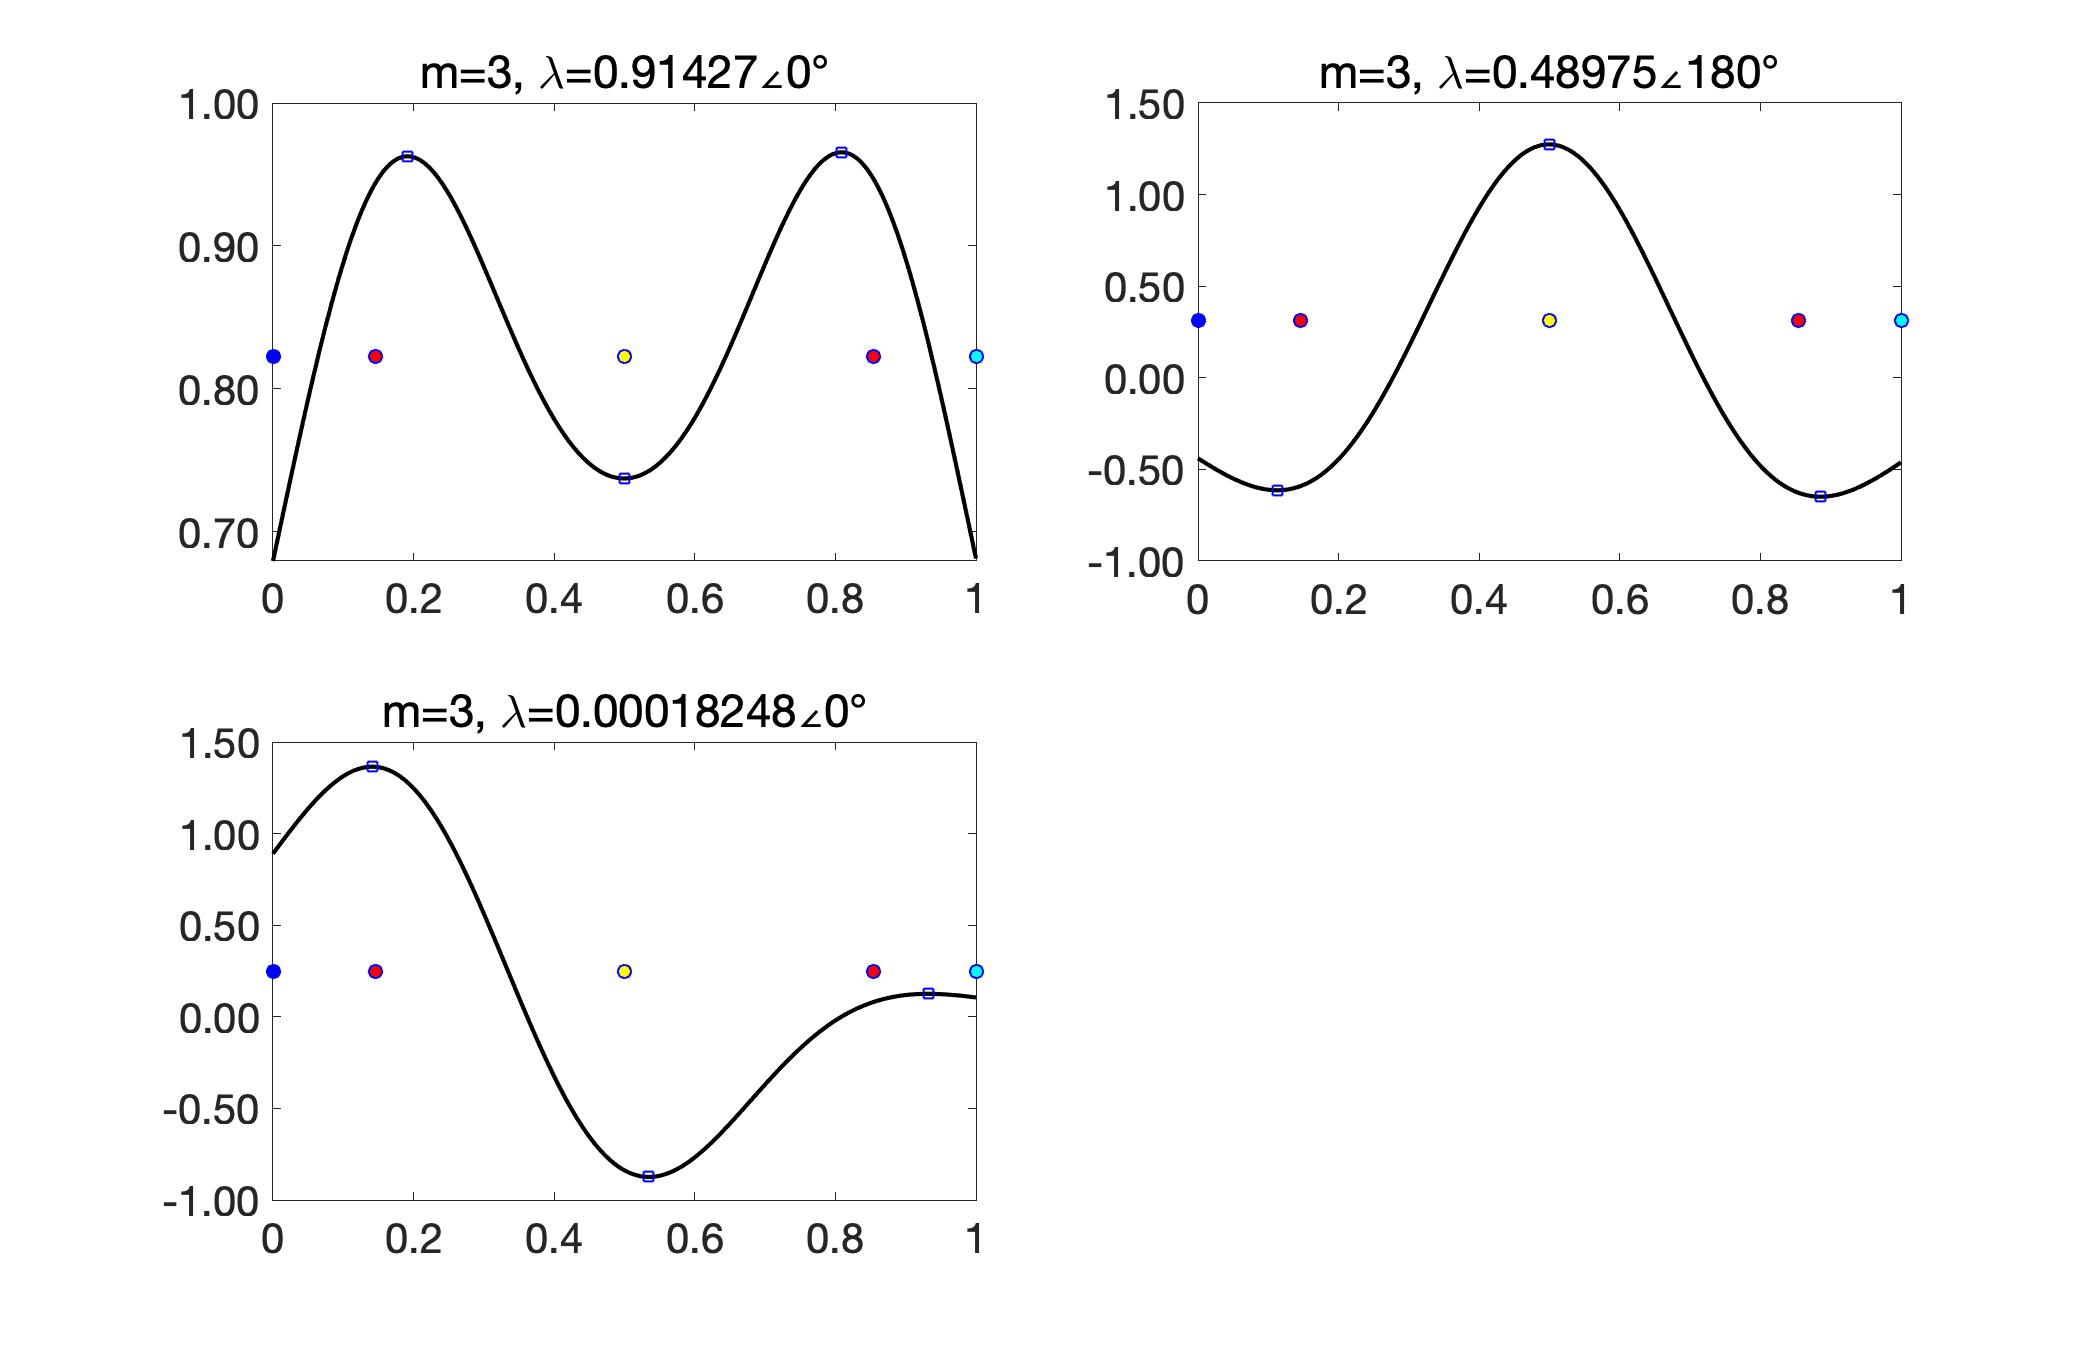
\includegraphics[scale=0.2]{logistic/noise/Logistic_eigen_noise_Gauss_d0-01_n1000_m3}}
      \\
    \subfloat[m=4]{
      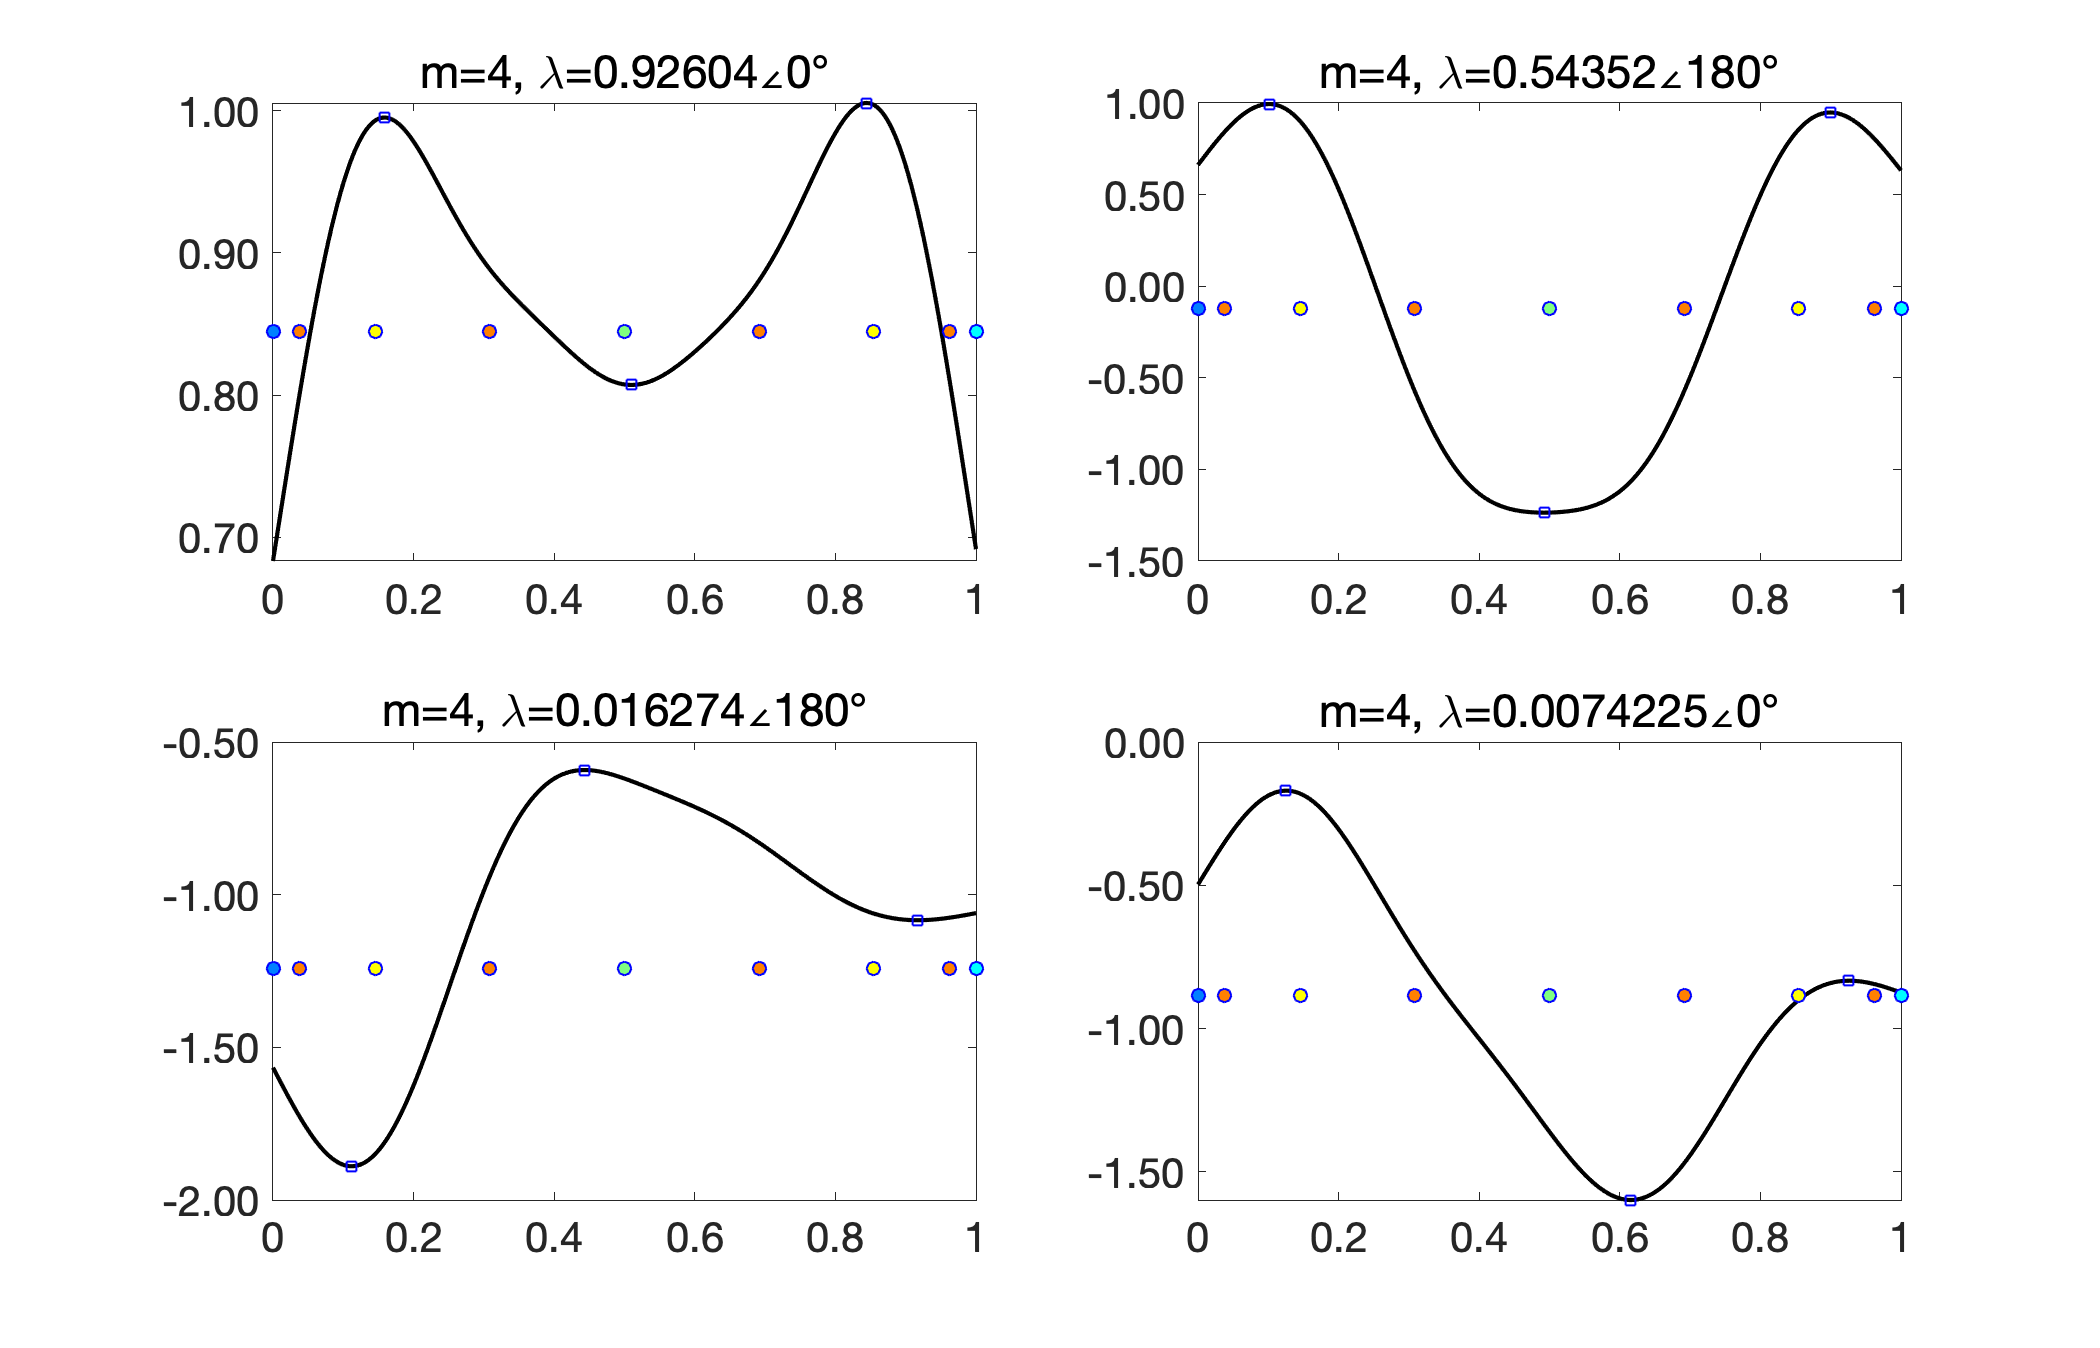
\includegraphics[scale=0.2]{logistic/noise/Logistic_eigen_noise_Gauss_d0-01_n1000_m4}}
    \subfloat[m=5]{
      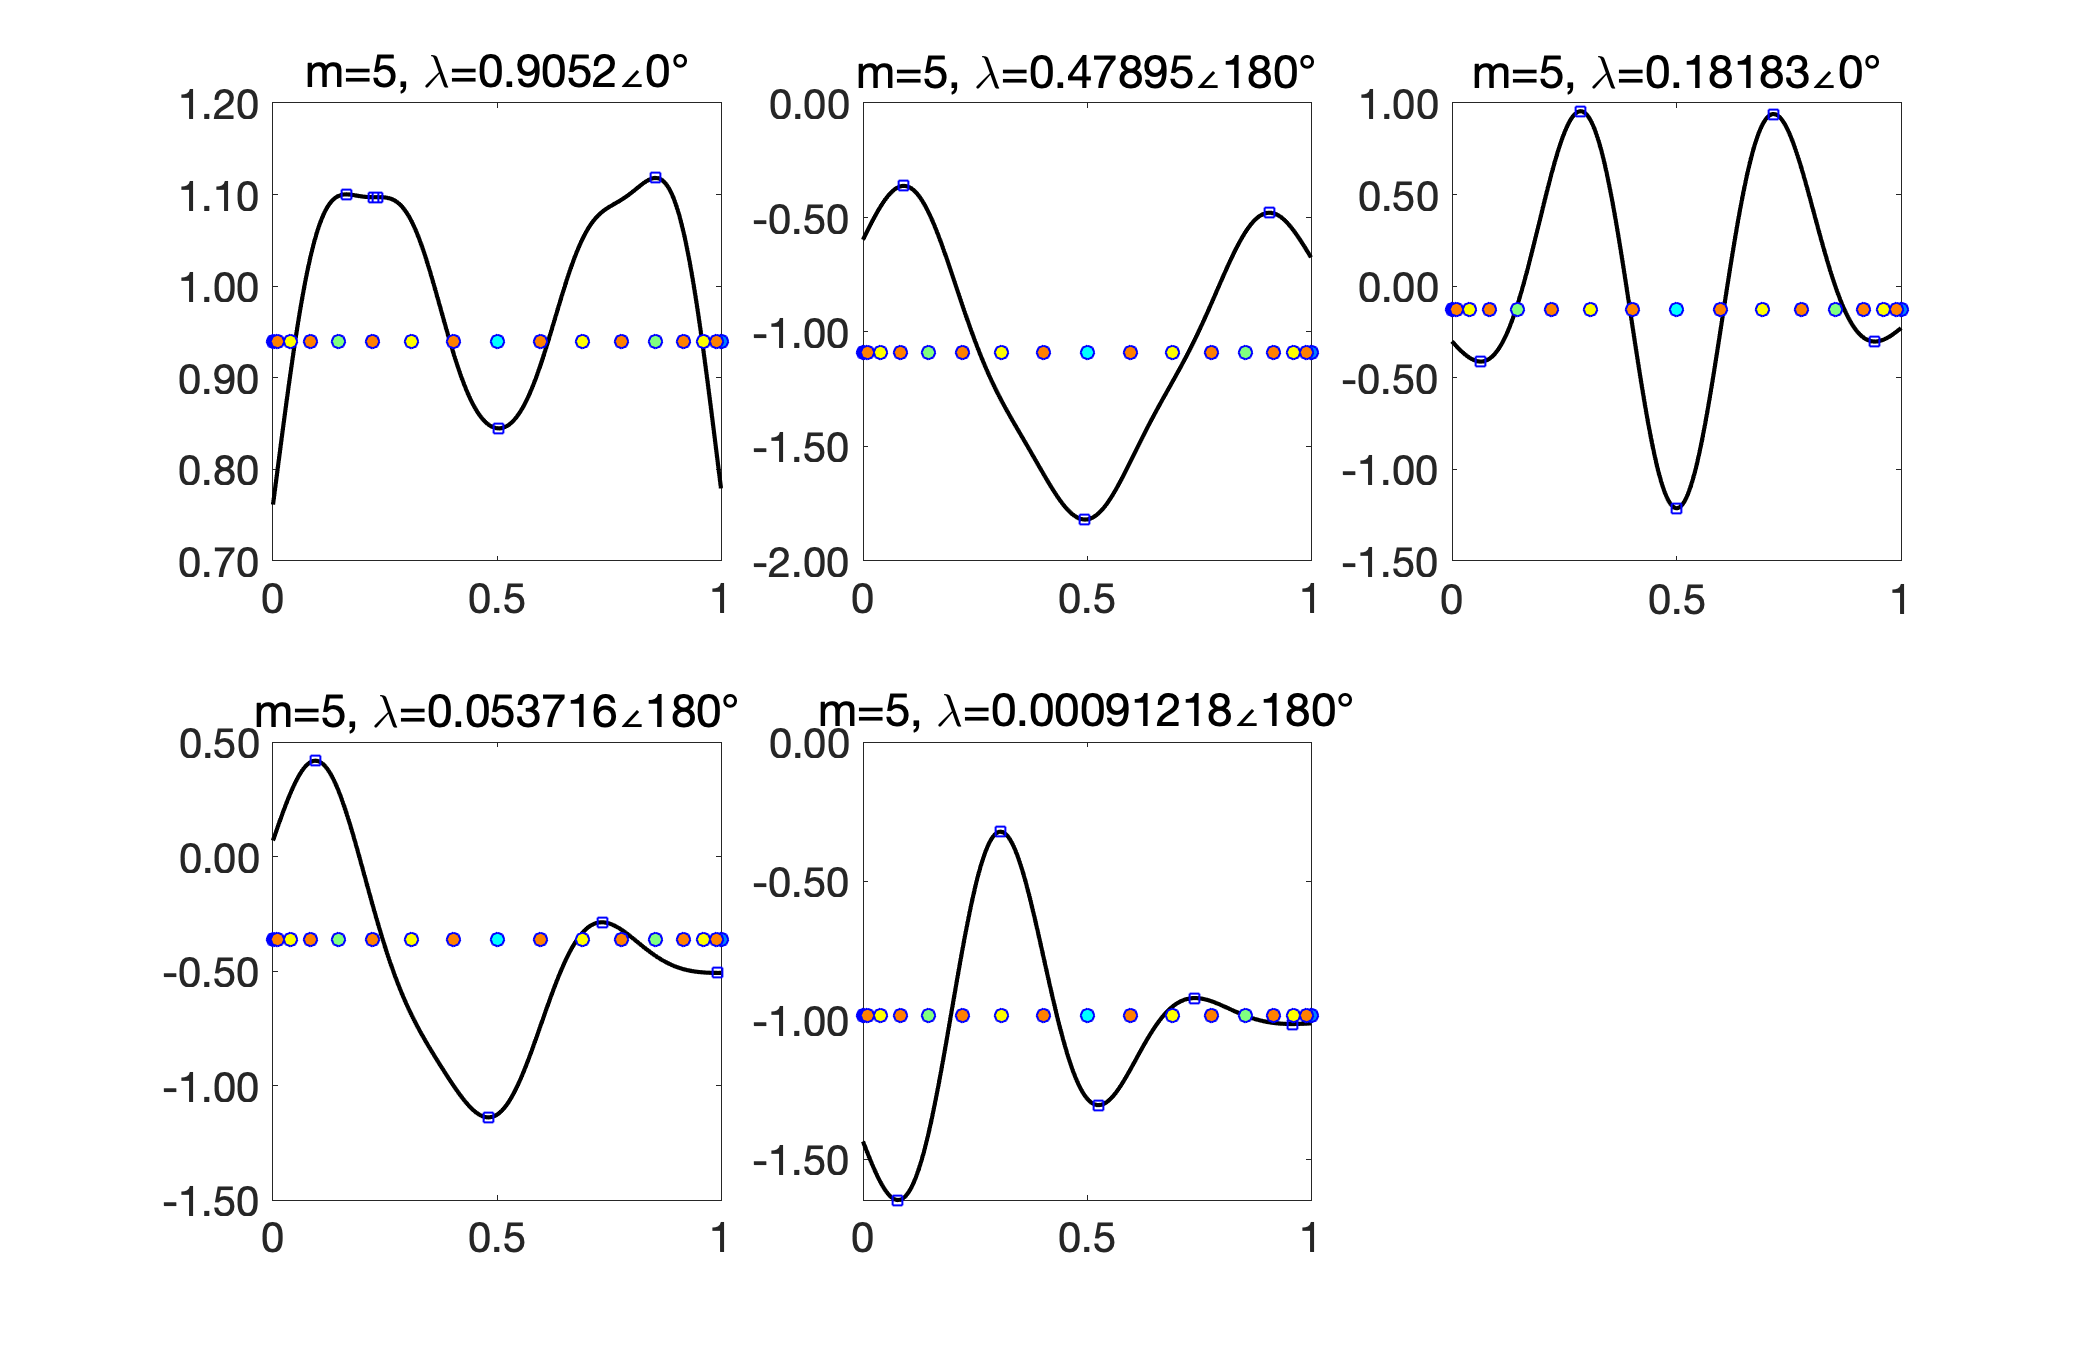
\includegraphics[scale=0.2]{logistic/noise/Logistic_eigen_noise_Gauss_d0-01_n1000_m5}}
      \\
    \subfloat[m=8]{
      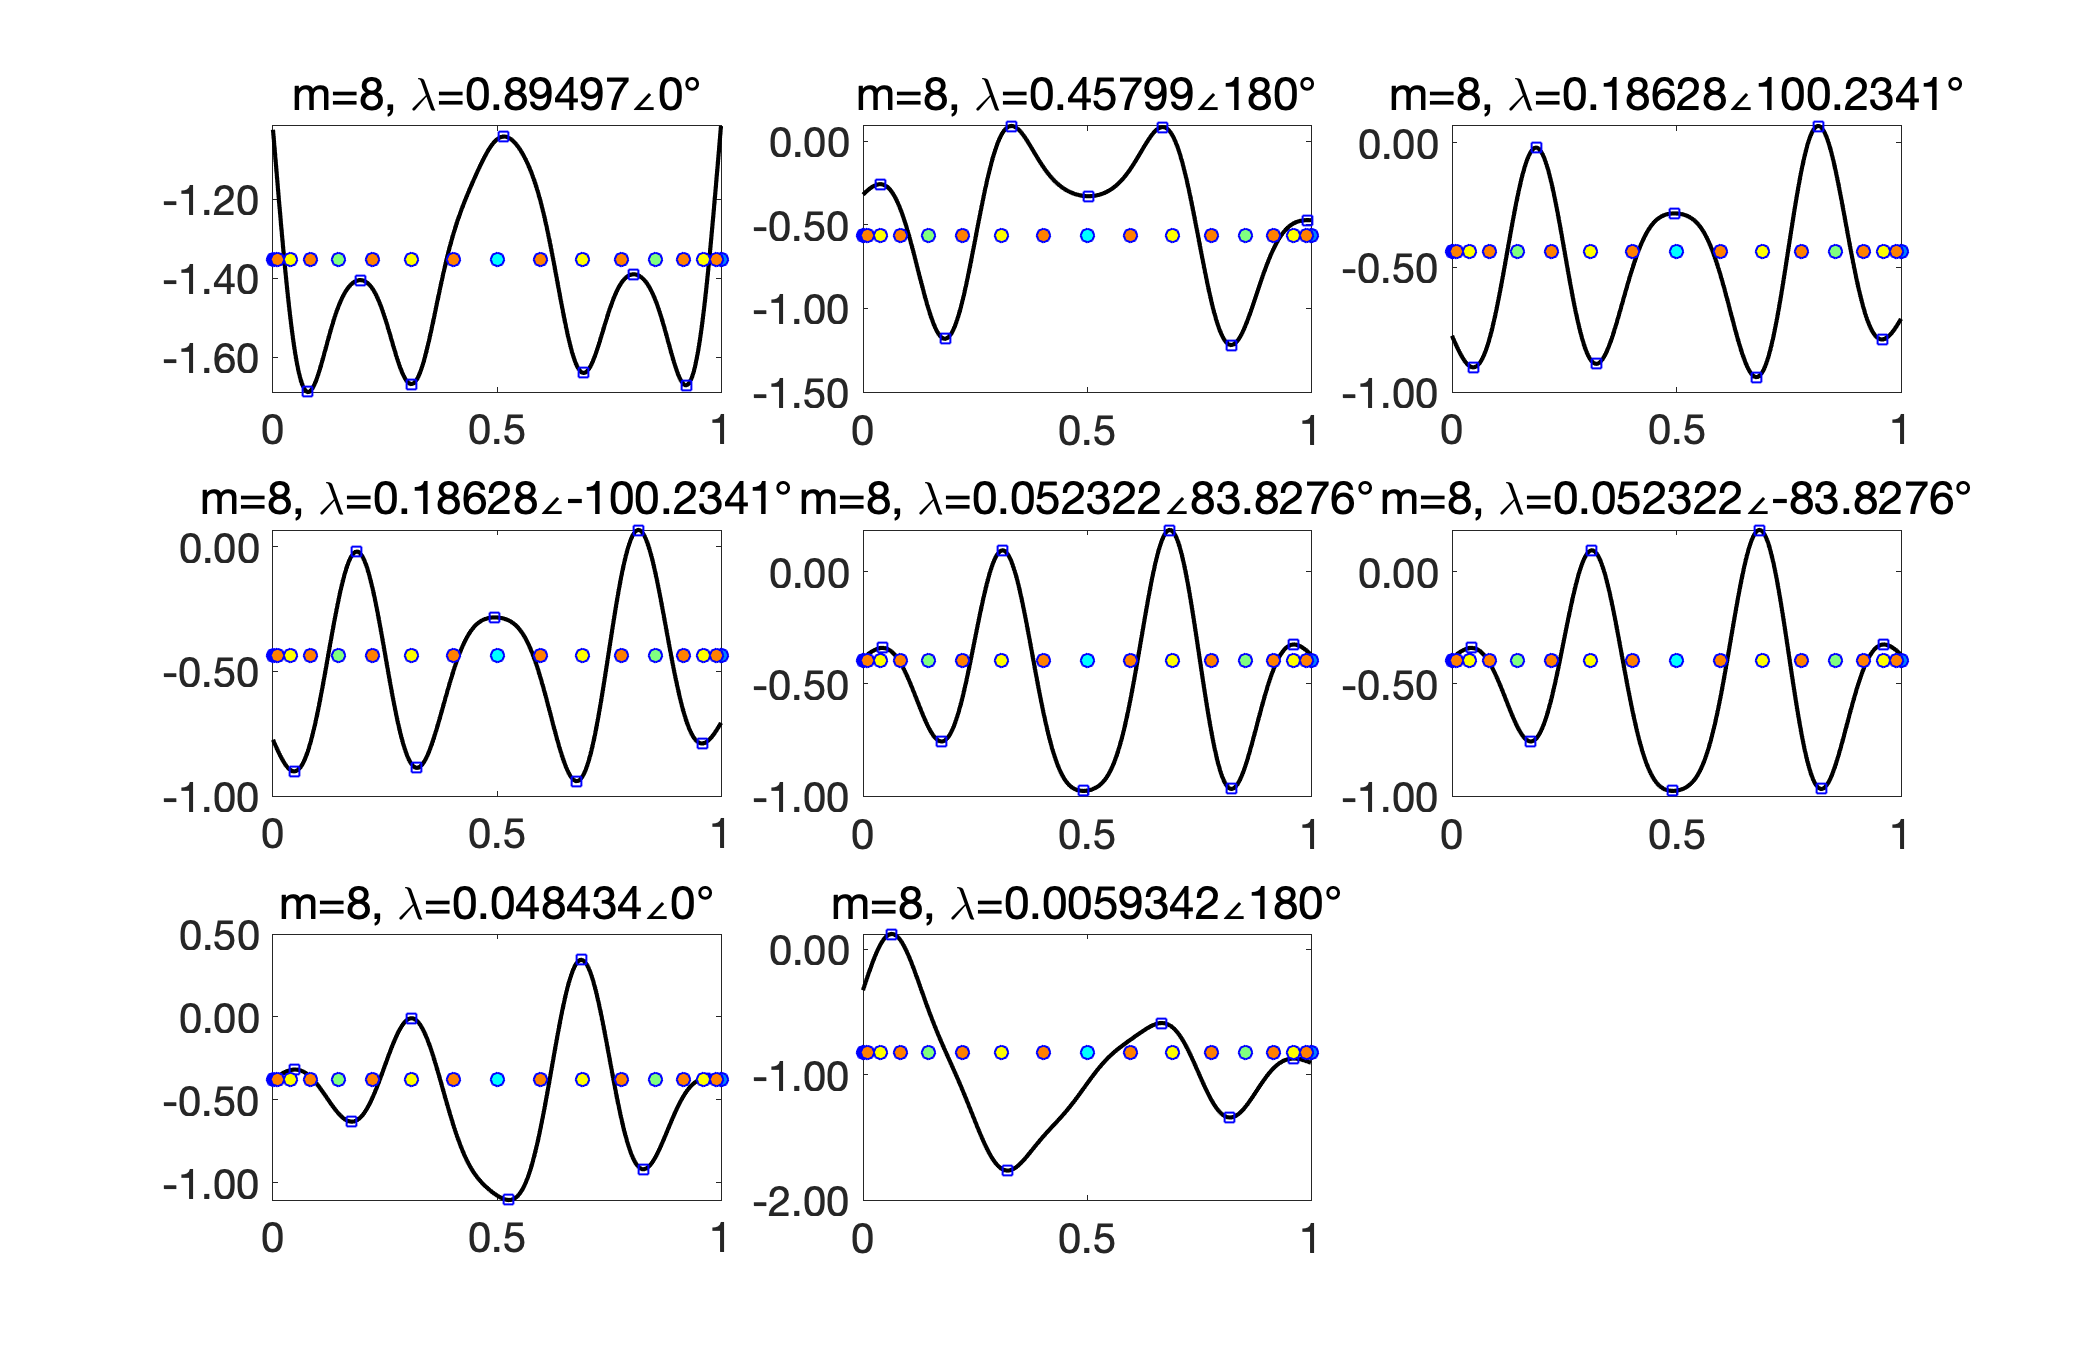
\includegraphics[scale=0.2]{logistic/noise/Logistic_eigen_noise_Gauss_d0-01_n1000_m8}}
    \subfloat[m=10]{
      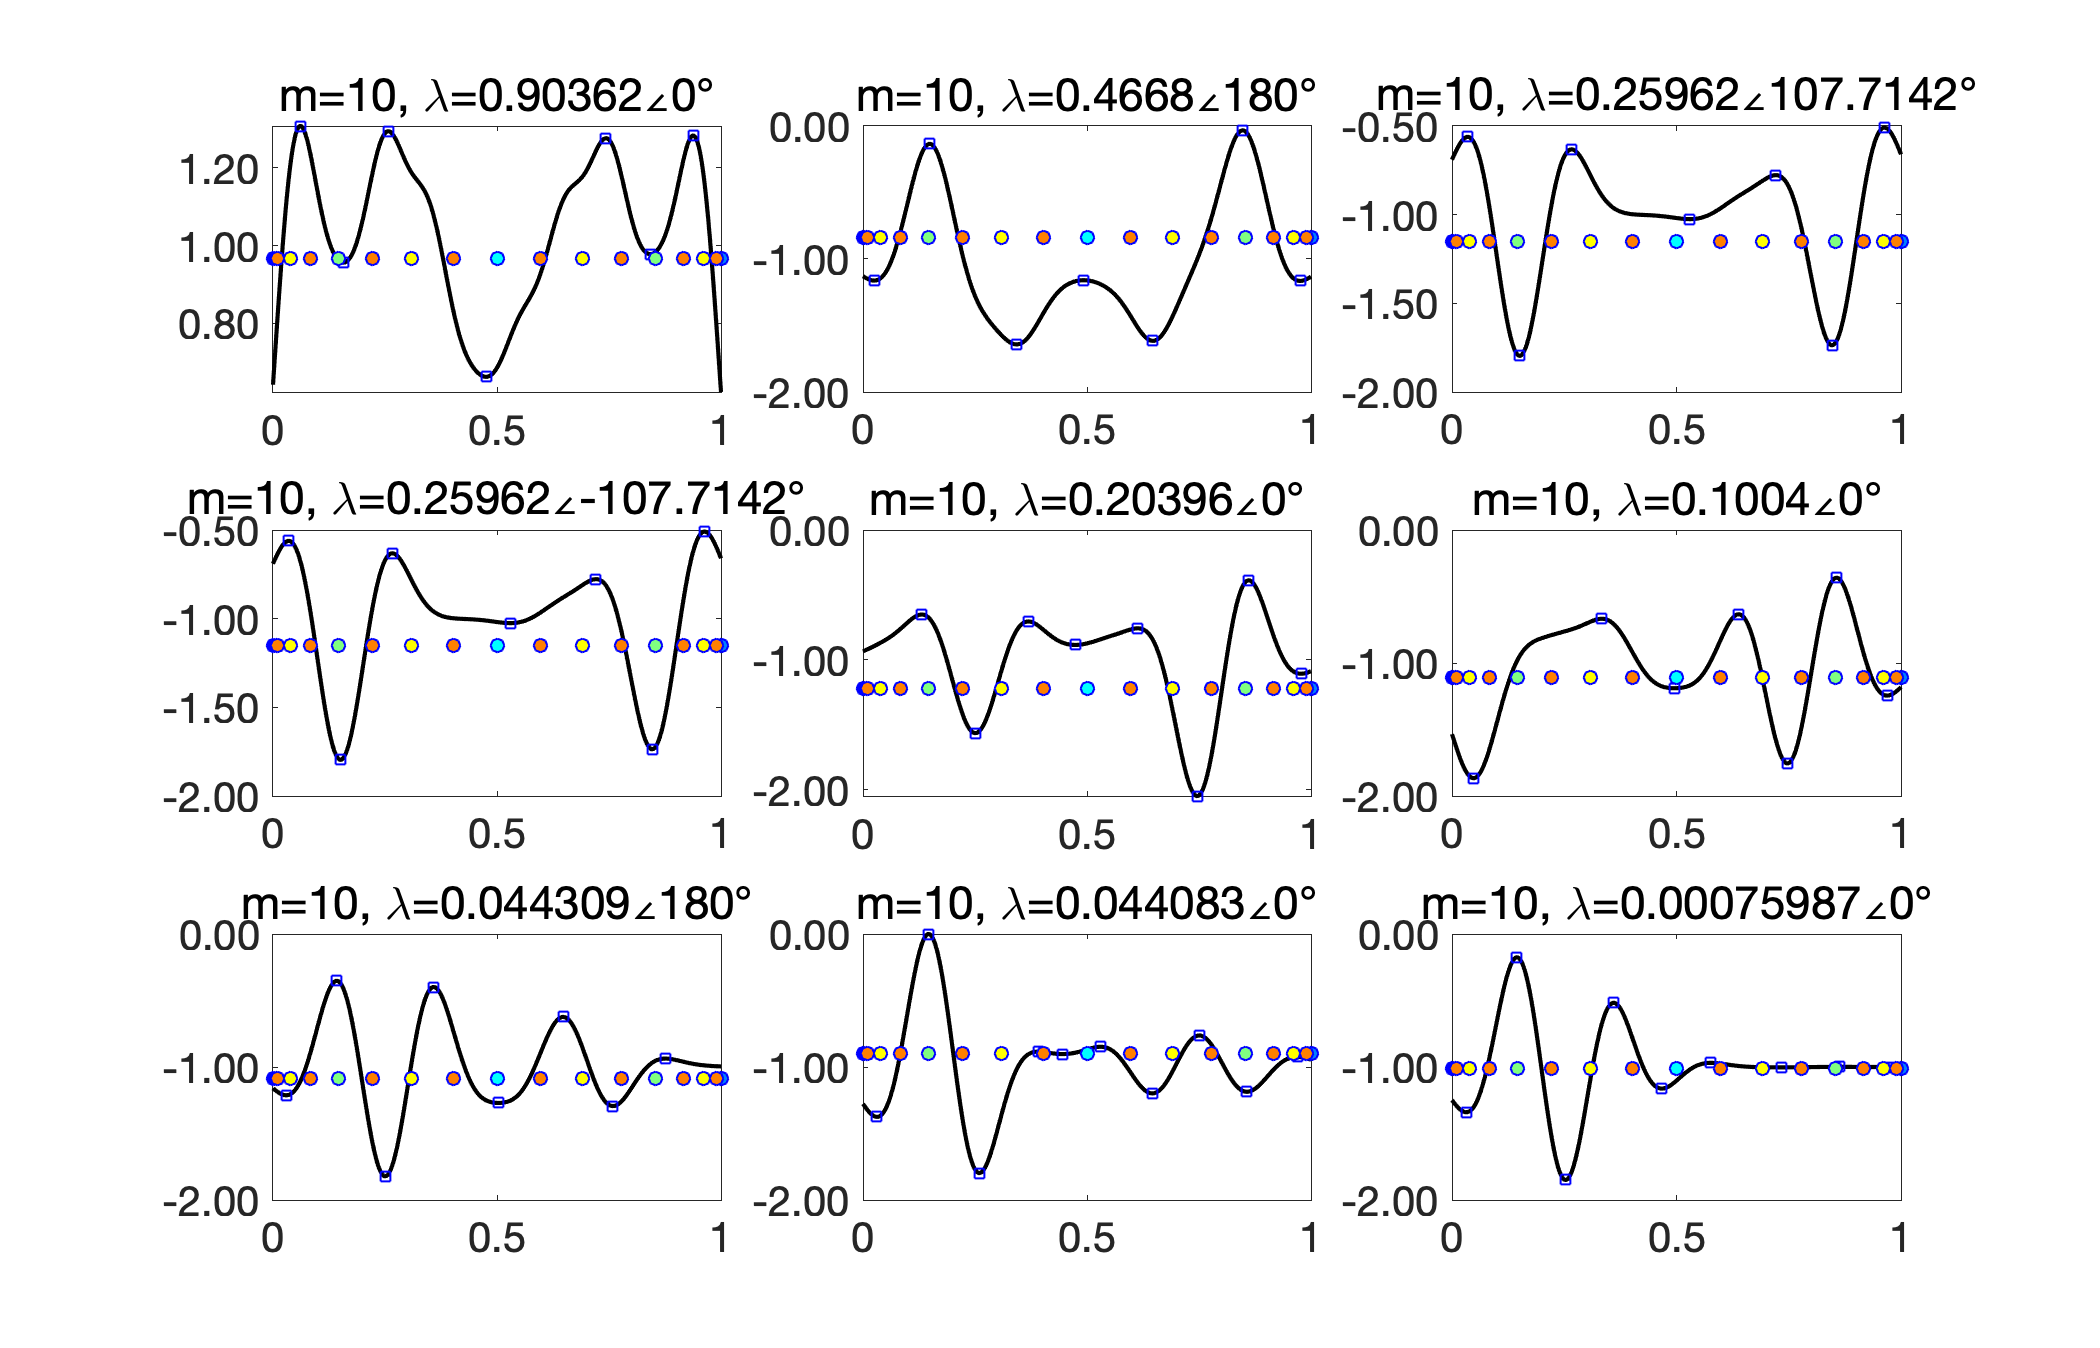
\includegraphics[scale=0.2]{logistic/noise/Logistic_eigen_noise_Gauss_d0-01_n1000_m10}}
      \\
    \subfloat[m=15]{
      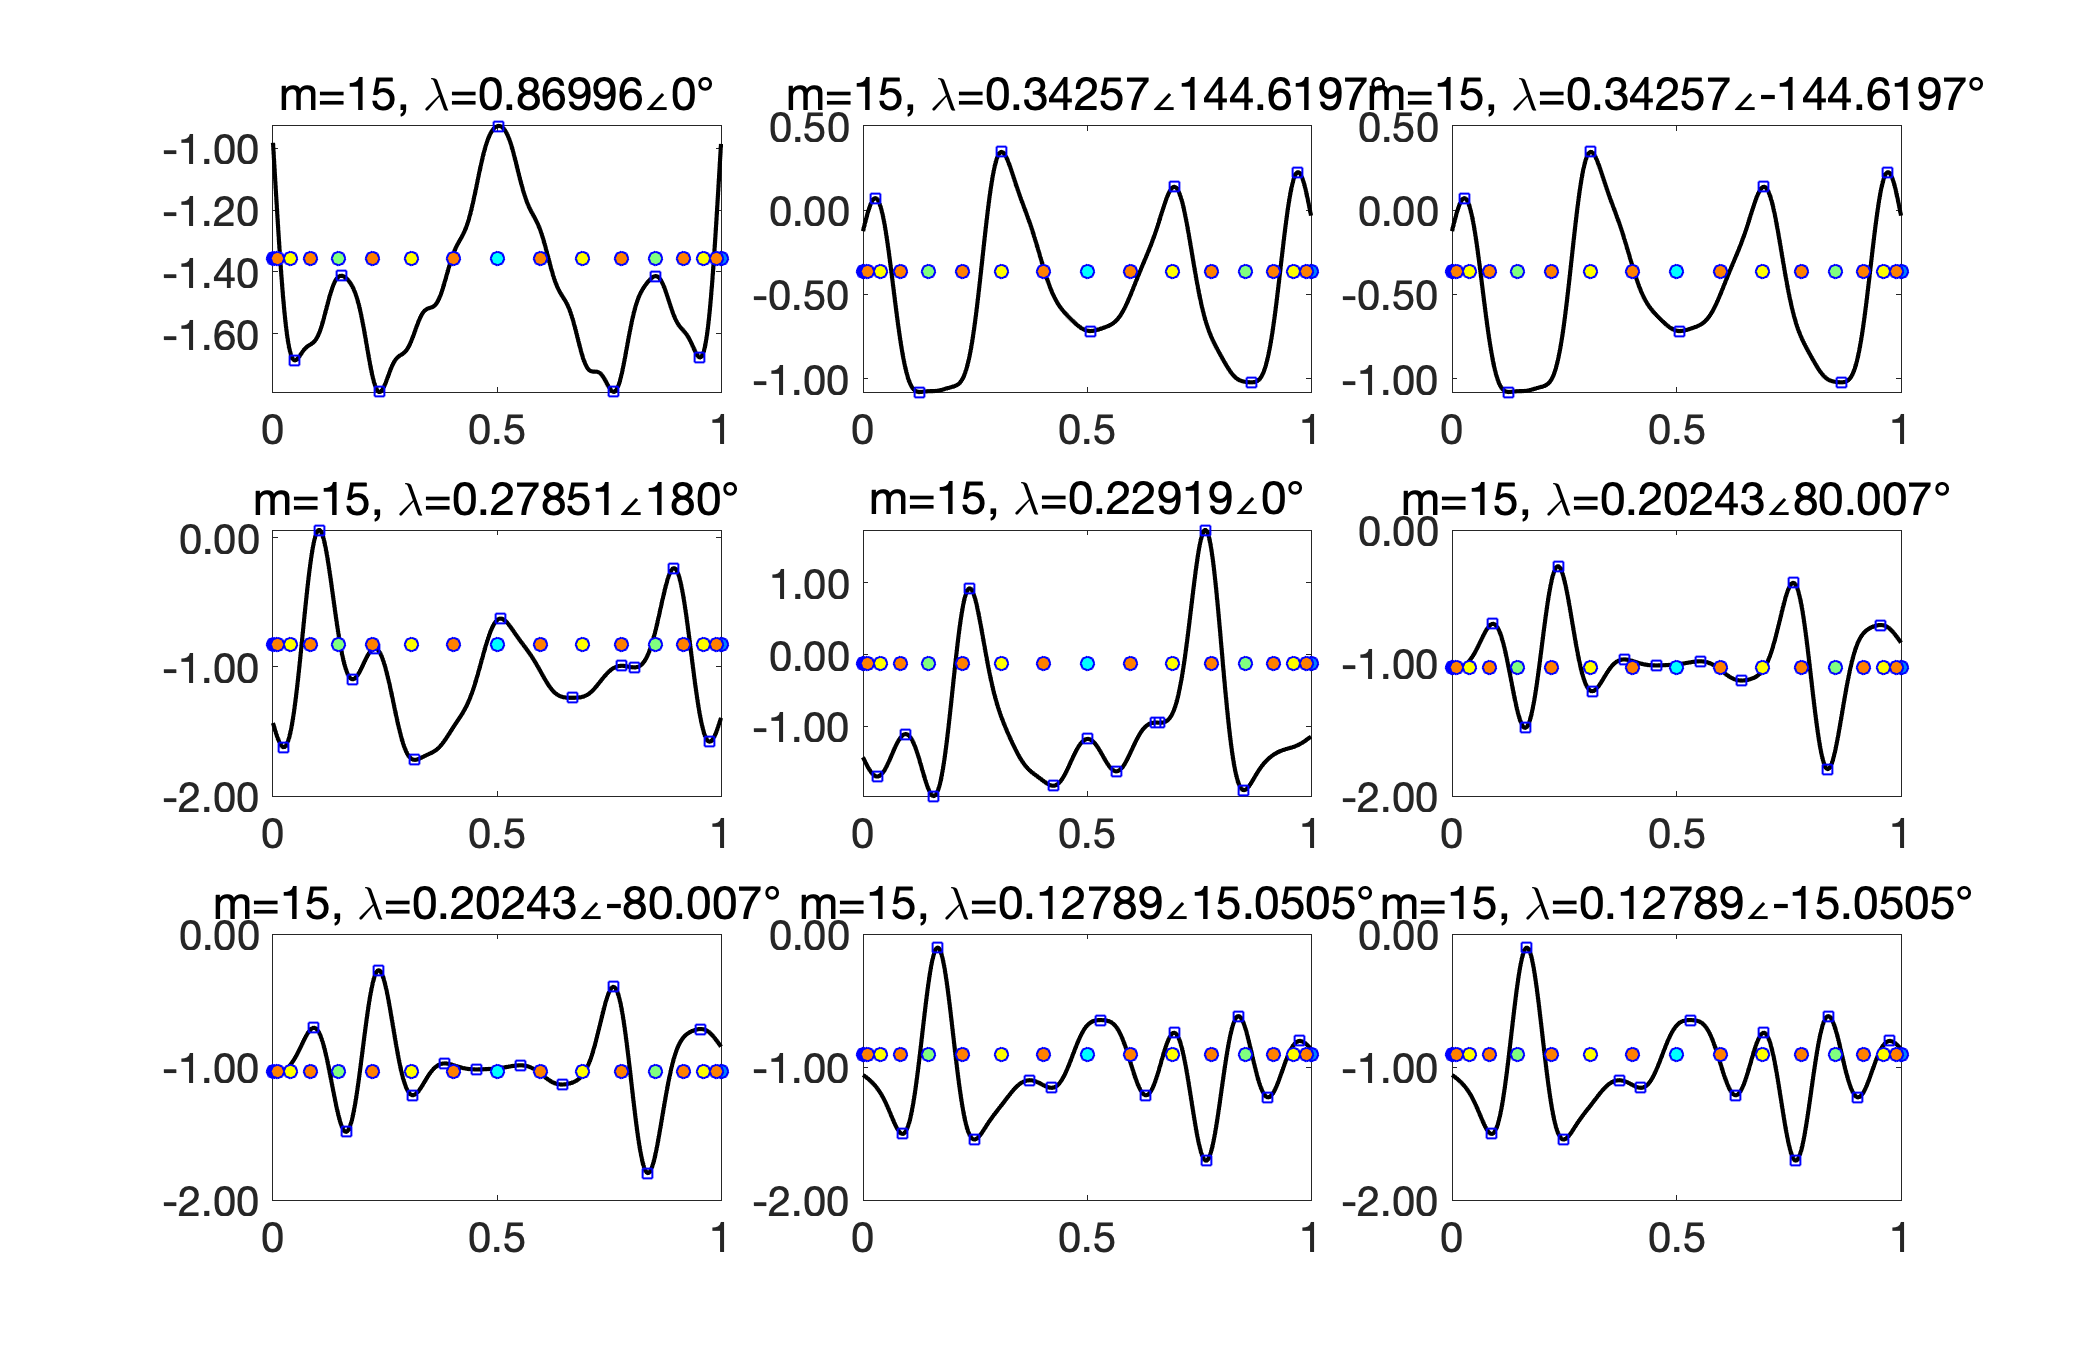
\includegraphics[scale=0.2]{logistic/noise/Logistic_eigen_noise_Gauss_d0-01_n1000_m15}}
    \subfloat[m=20]{
      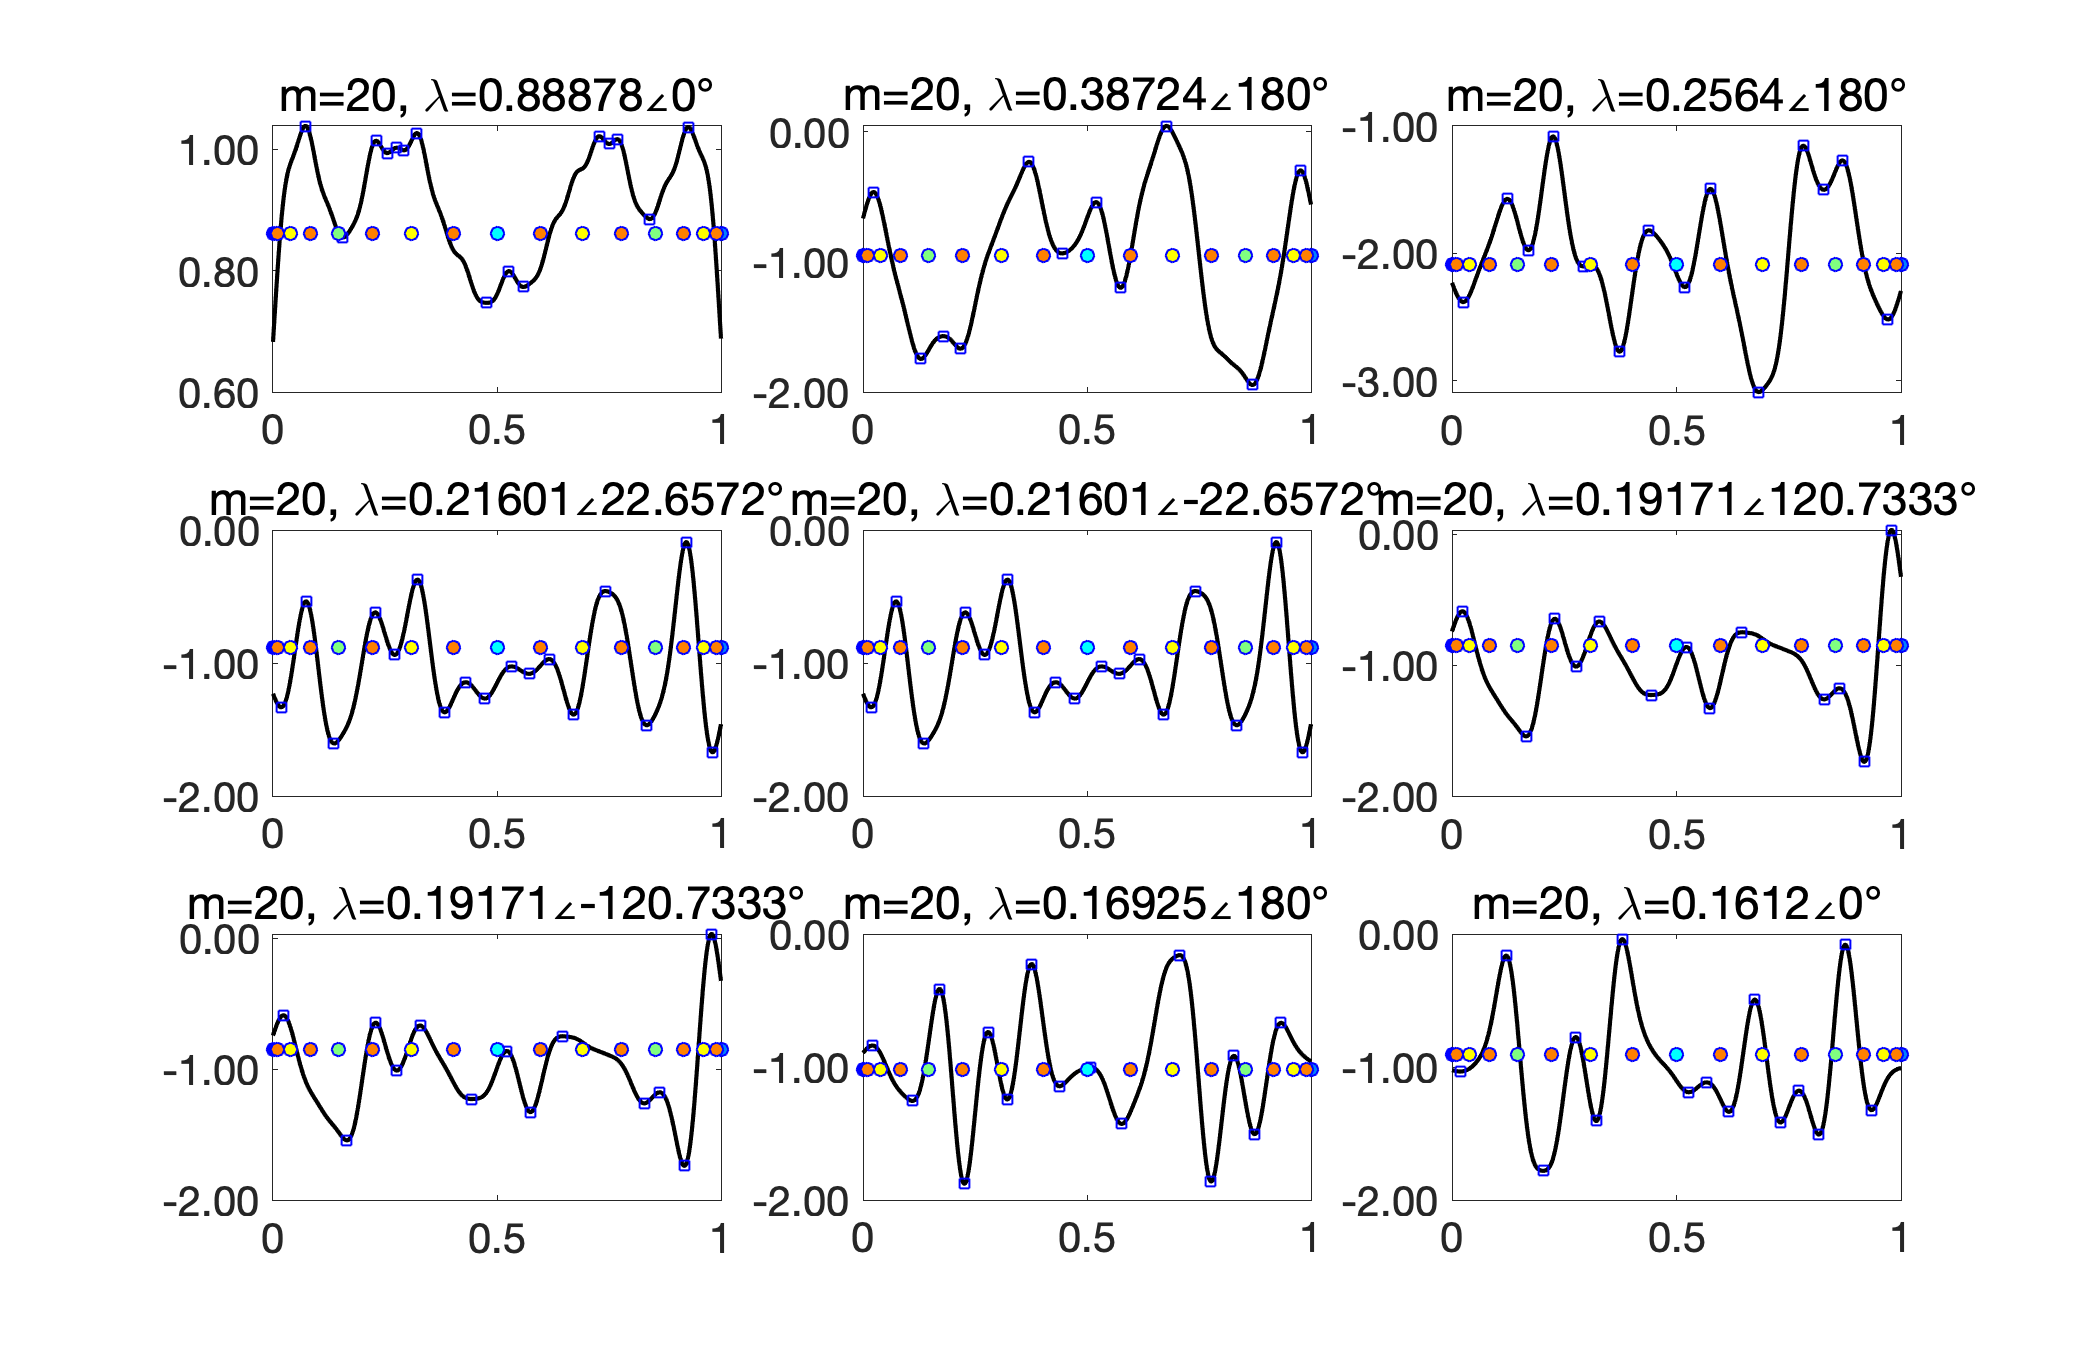
\includegraphics[scale=0.2]{logistic/noise/Logistic_eigen_noise_Gauss_d0-01_n1000_m20}}
      \\
      \caption{Logistic映射的边界点与本征函数($noise=0.01$)}\label{fig:Logistic_eigen_noise_n1000m20d0-01}
\end{figure}

在图\ref{fig:Logistic_eigen_noise_n1000m20d0-001}(a)第二个小图中,我们观察到由于噪声项的影响,Koopman算符的本征函数的极值点与边界点$x=\frac{1}{2}$会有一定距离的偏移,随着基函数数量的增加,本征函数的细节上会有些许变化,但是大致趋势并未发生明显的变化。图\ref{fig:Logistic_eigen_noise_n1000m20d0-01}中增加了噪声的大小$noise=0.01$,本征函数图像变得更不规则了,但总体观察Koopman算符本征函数的极值点,其噪声对其划分边界点的影响并不大。如在图\ref{fig:Logistic_eigen_noise_n1000m20d0-01}(h)第四个小图中,本征函数的细节变的稍稍不规则,但是在边界点$x=\frac{1}{2}$附近处与边界点$x=0.1464,0.8536$处同样存在较明显的本征函数极值点,且处于不同层次。综上我们可以确定,Koopman算符的本征函数的极值点对边界点的划分这一结论是具有鲁棒性的,与帐篷映射中的结论一致。

同样,我们要验证随着基函数的增加,本征函数是否能更精确的划分我们的边界点。在两个基函数数量$m_1$和$m_2$下通过本征函数$\phi_{m_1}$来确定$\phi_{m_2}$下的本征函数,利用函数最小值对应的参数问题(式\ref{equ:argmin}),及利用本征函数之间的相似性(式\ref{equ:cov_xy})。我们可以作出图\ref{fig:Logistic_findeigen_m8m16}中,我们根据寻找函数式\ref{equ:argmin}最小值进行了四组对比:$m=4,8$,$m=8,16$,$m=16,32$,$m=32,64$,在每个图中,蓝色的线表示较小的基函数数量下的本征函数,我们以此蓝色的本征函数$\phi_{m_1}$为基础,根据式\ref{equ:argmin}计算得到较大的基函数数量下的本征函数,即红色的本征函数$\phi_{m_2}$。

\begin{figure}[!]
  \centering
  \subfloat[m=4,8]{
    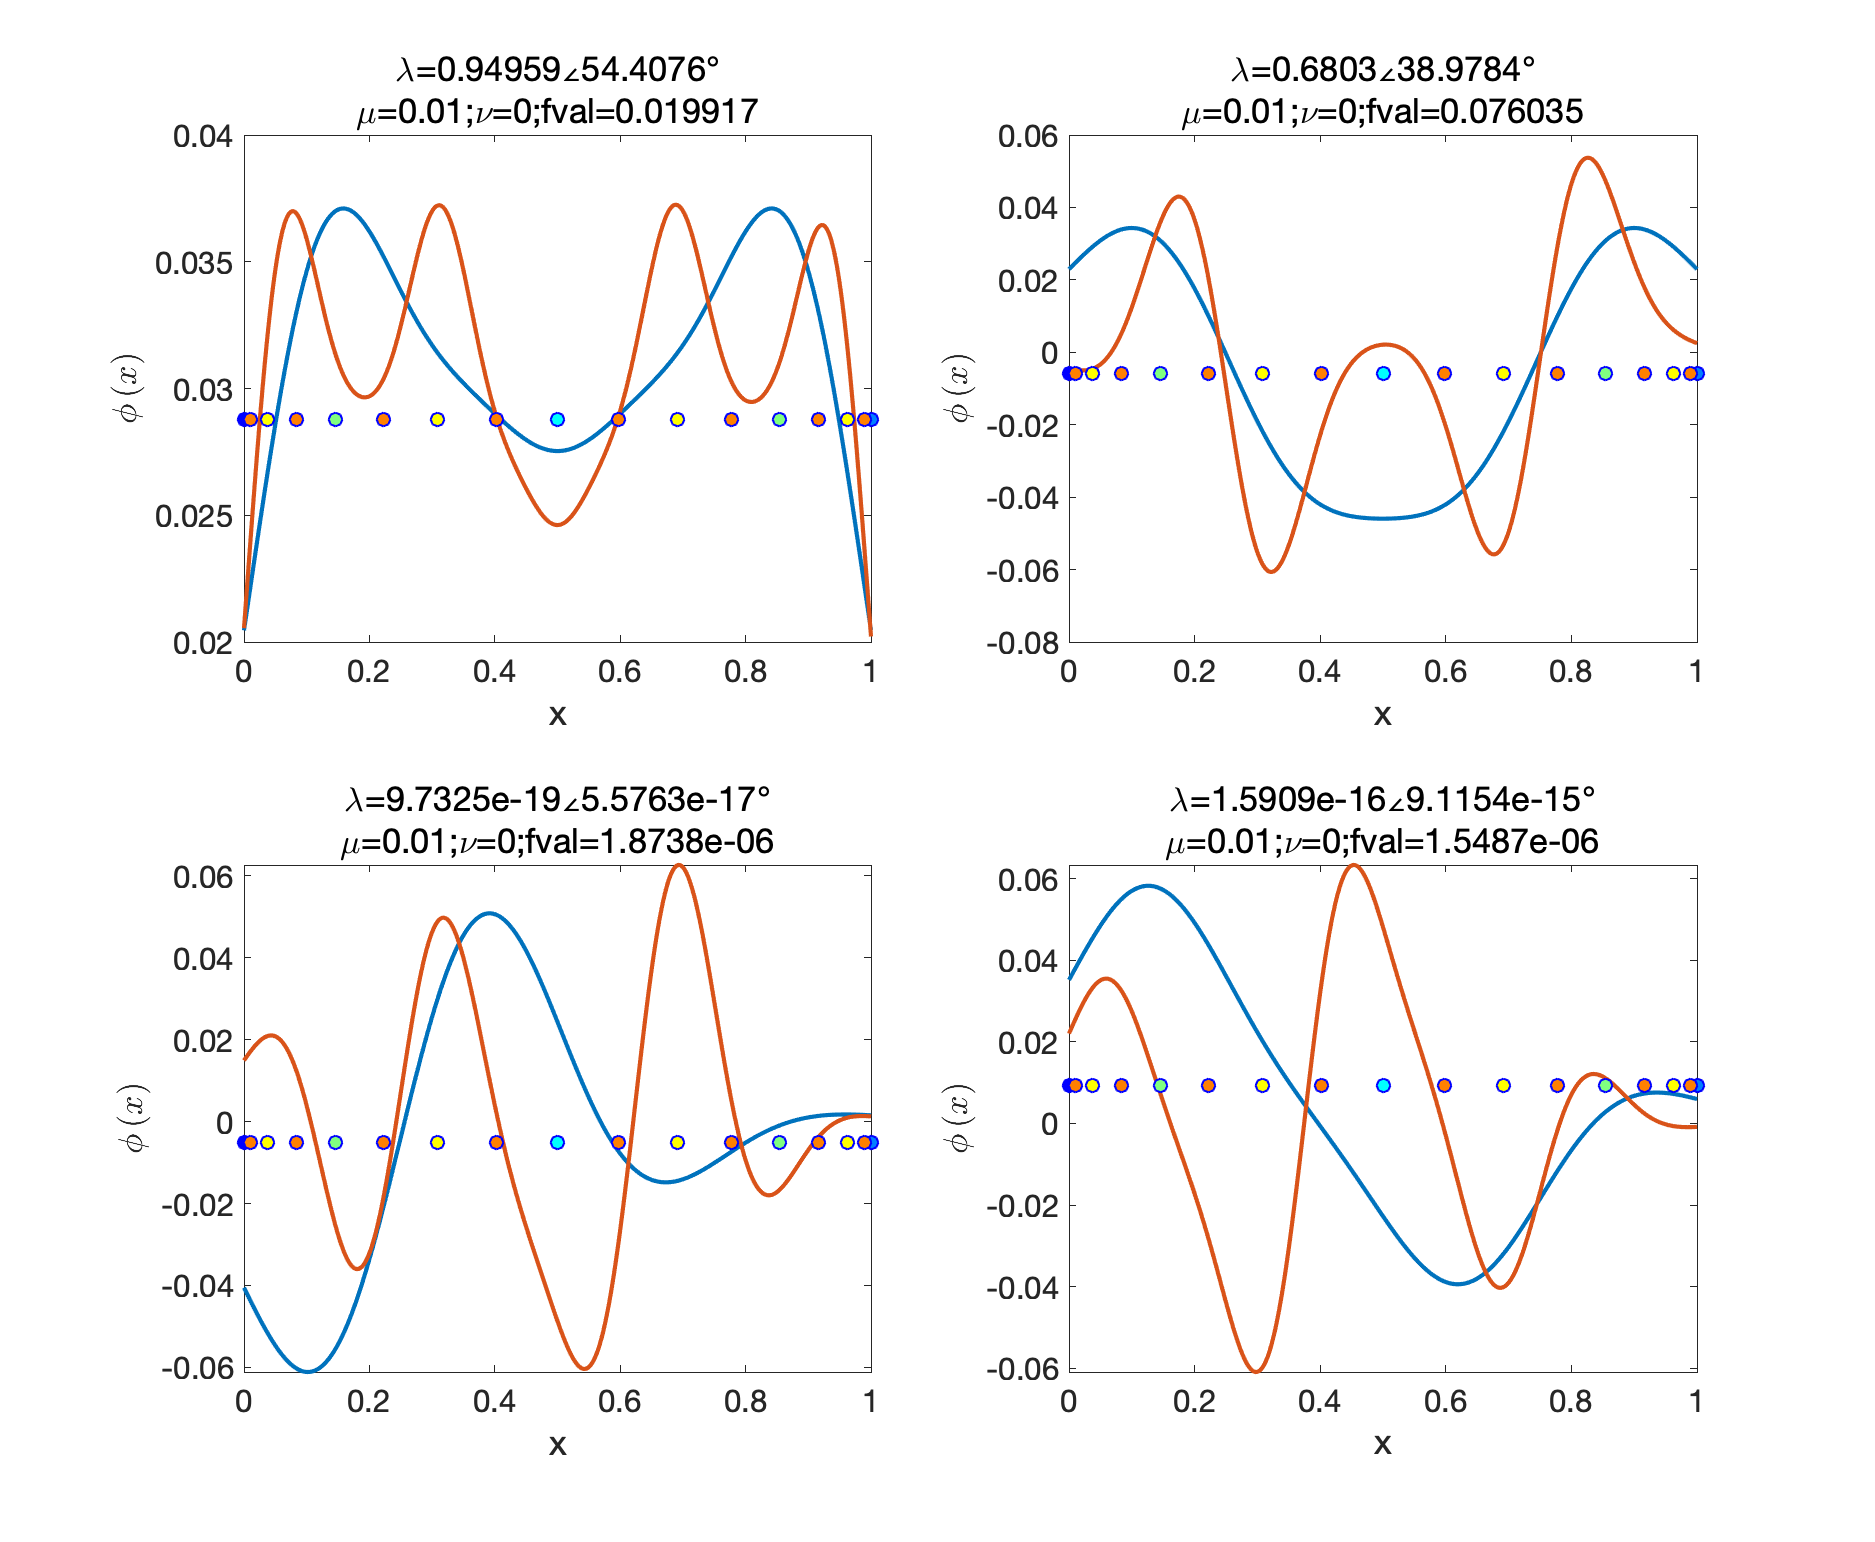
\includegraphics[scale=0.2]{logistic/accurate/Logistic_findeigen_m4m8}}
  \subfloat[m=8,16]{
    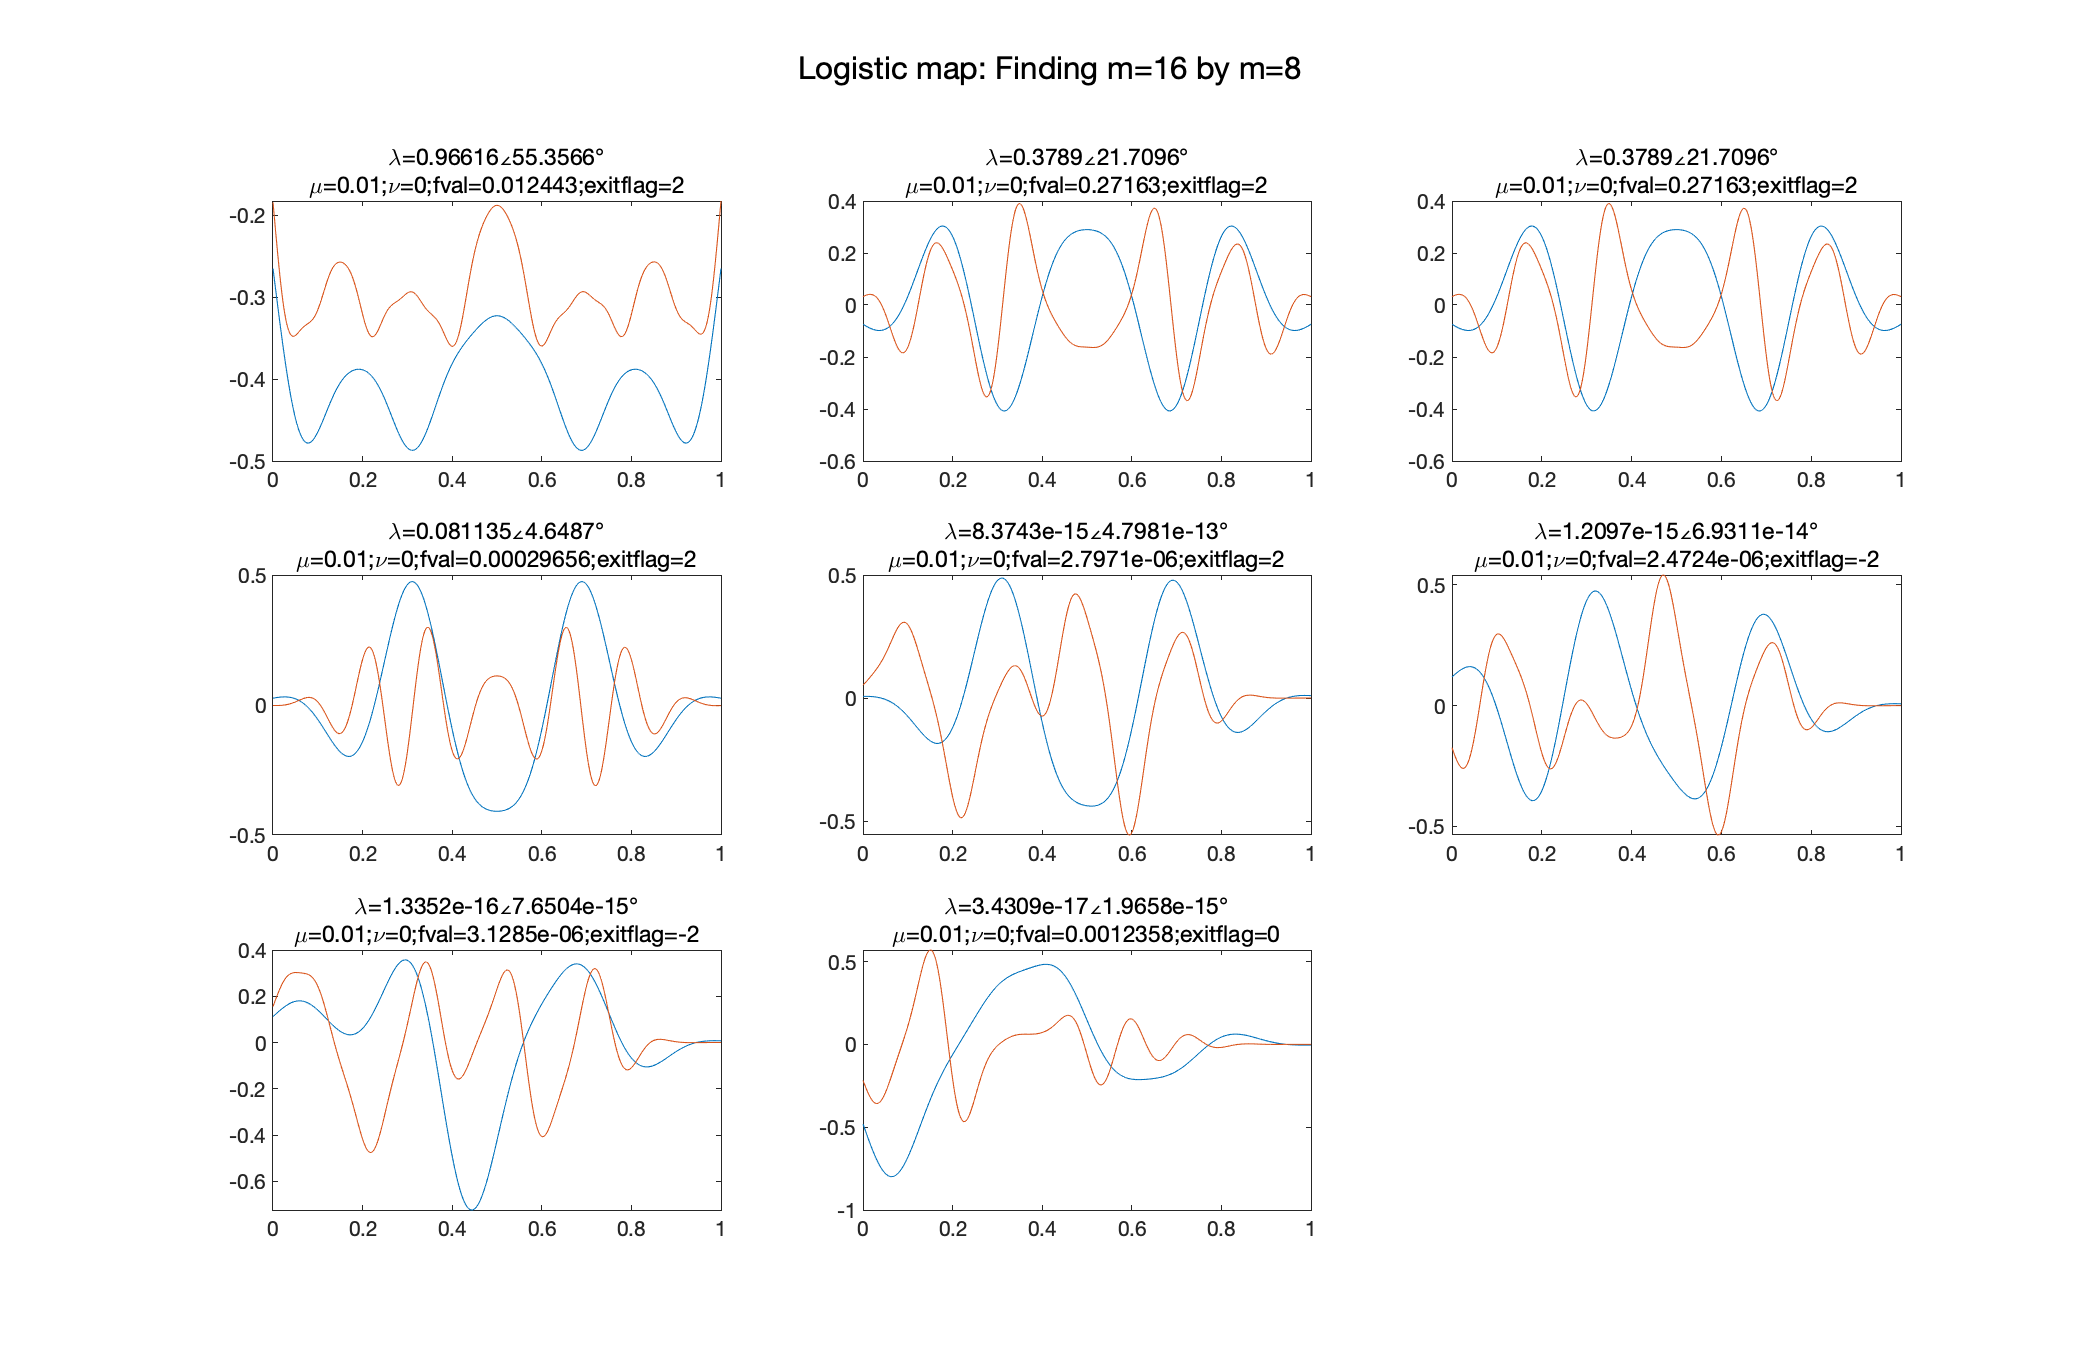
\includegraphics[scale=0.2]{logistic/accurate/Logistic_findeigen_m8m16}}
    \\
  \subfloat[m=16,32]{
    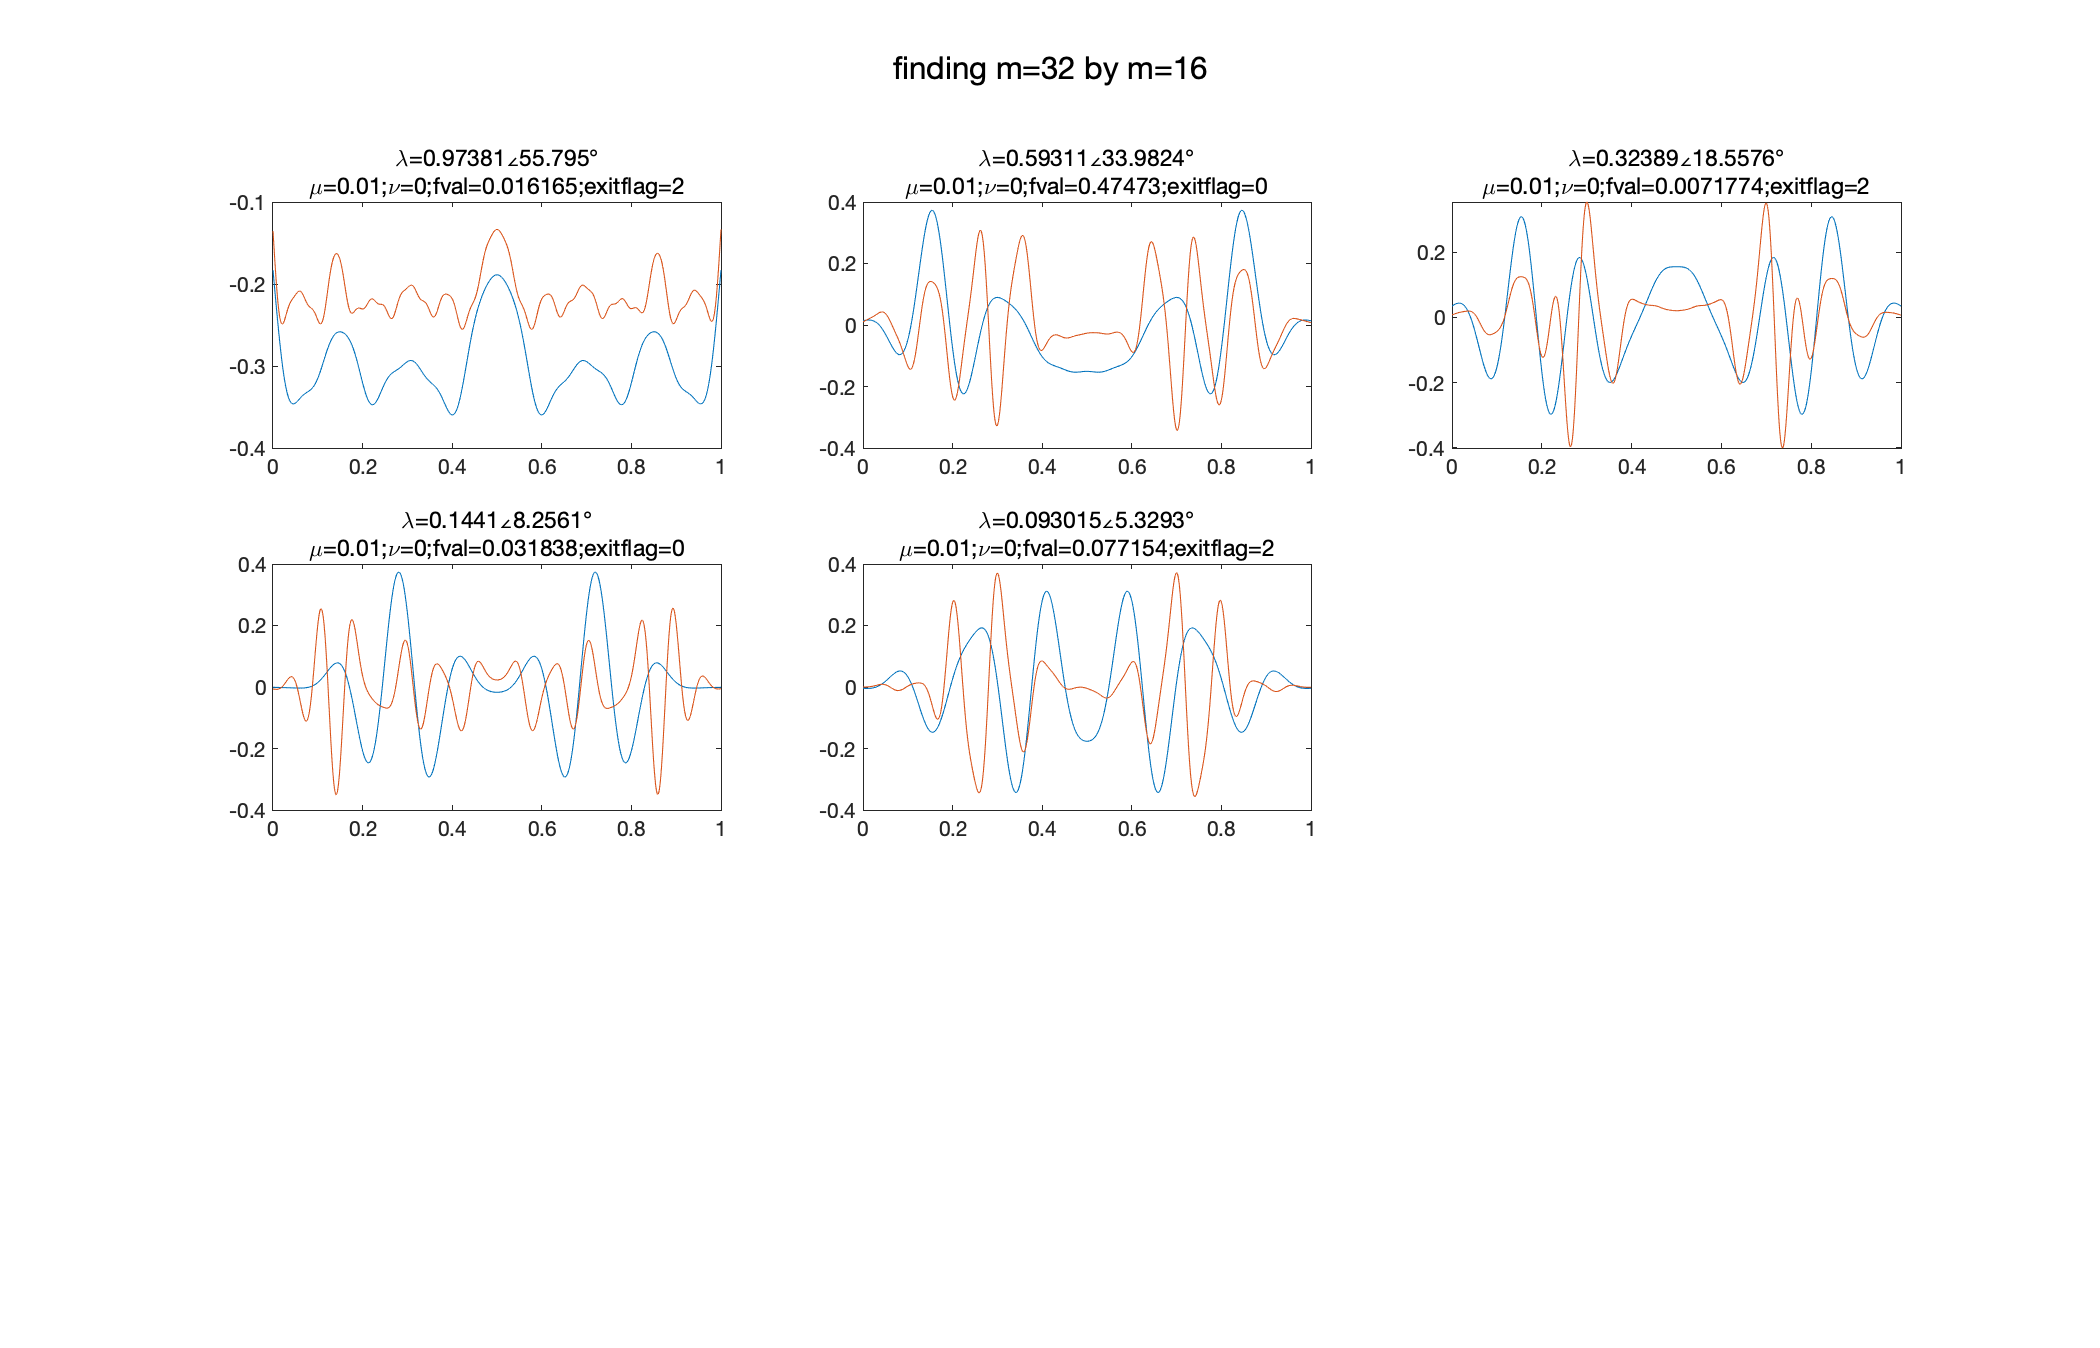
\includegraphics[scale=0.2]{logistic/accurate/Logistic_findeigen_m16m32}}
  \subfloat[m=32,64]{
    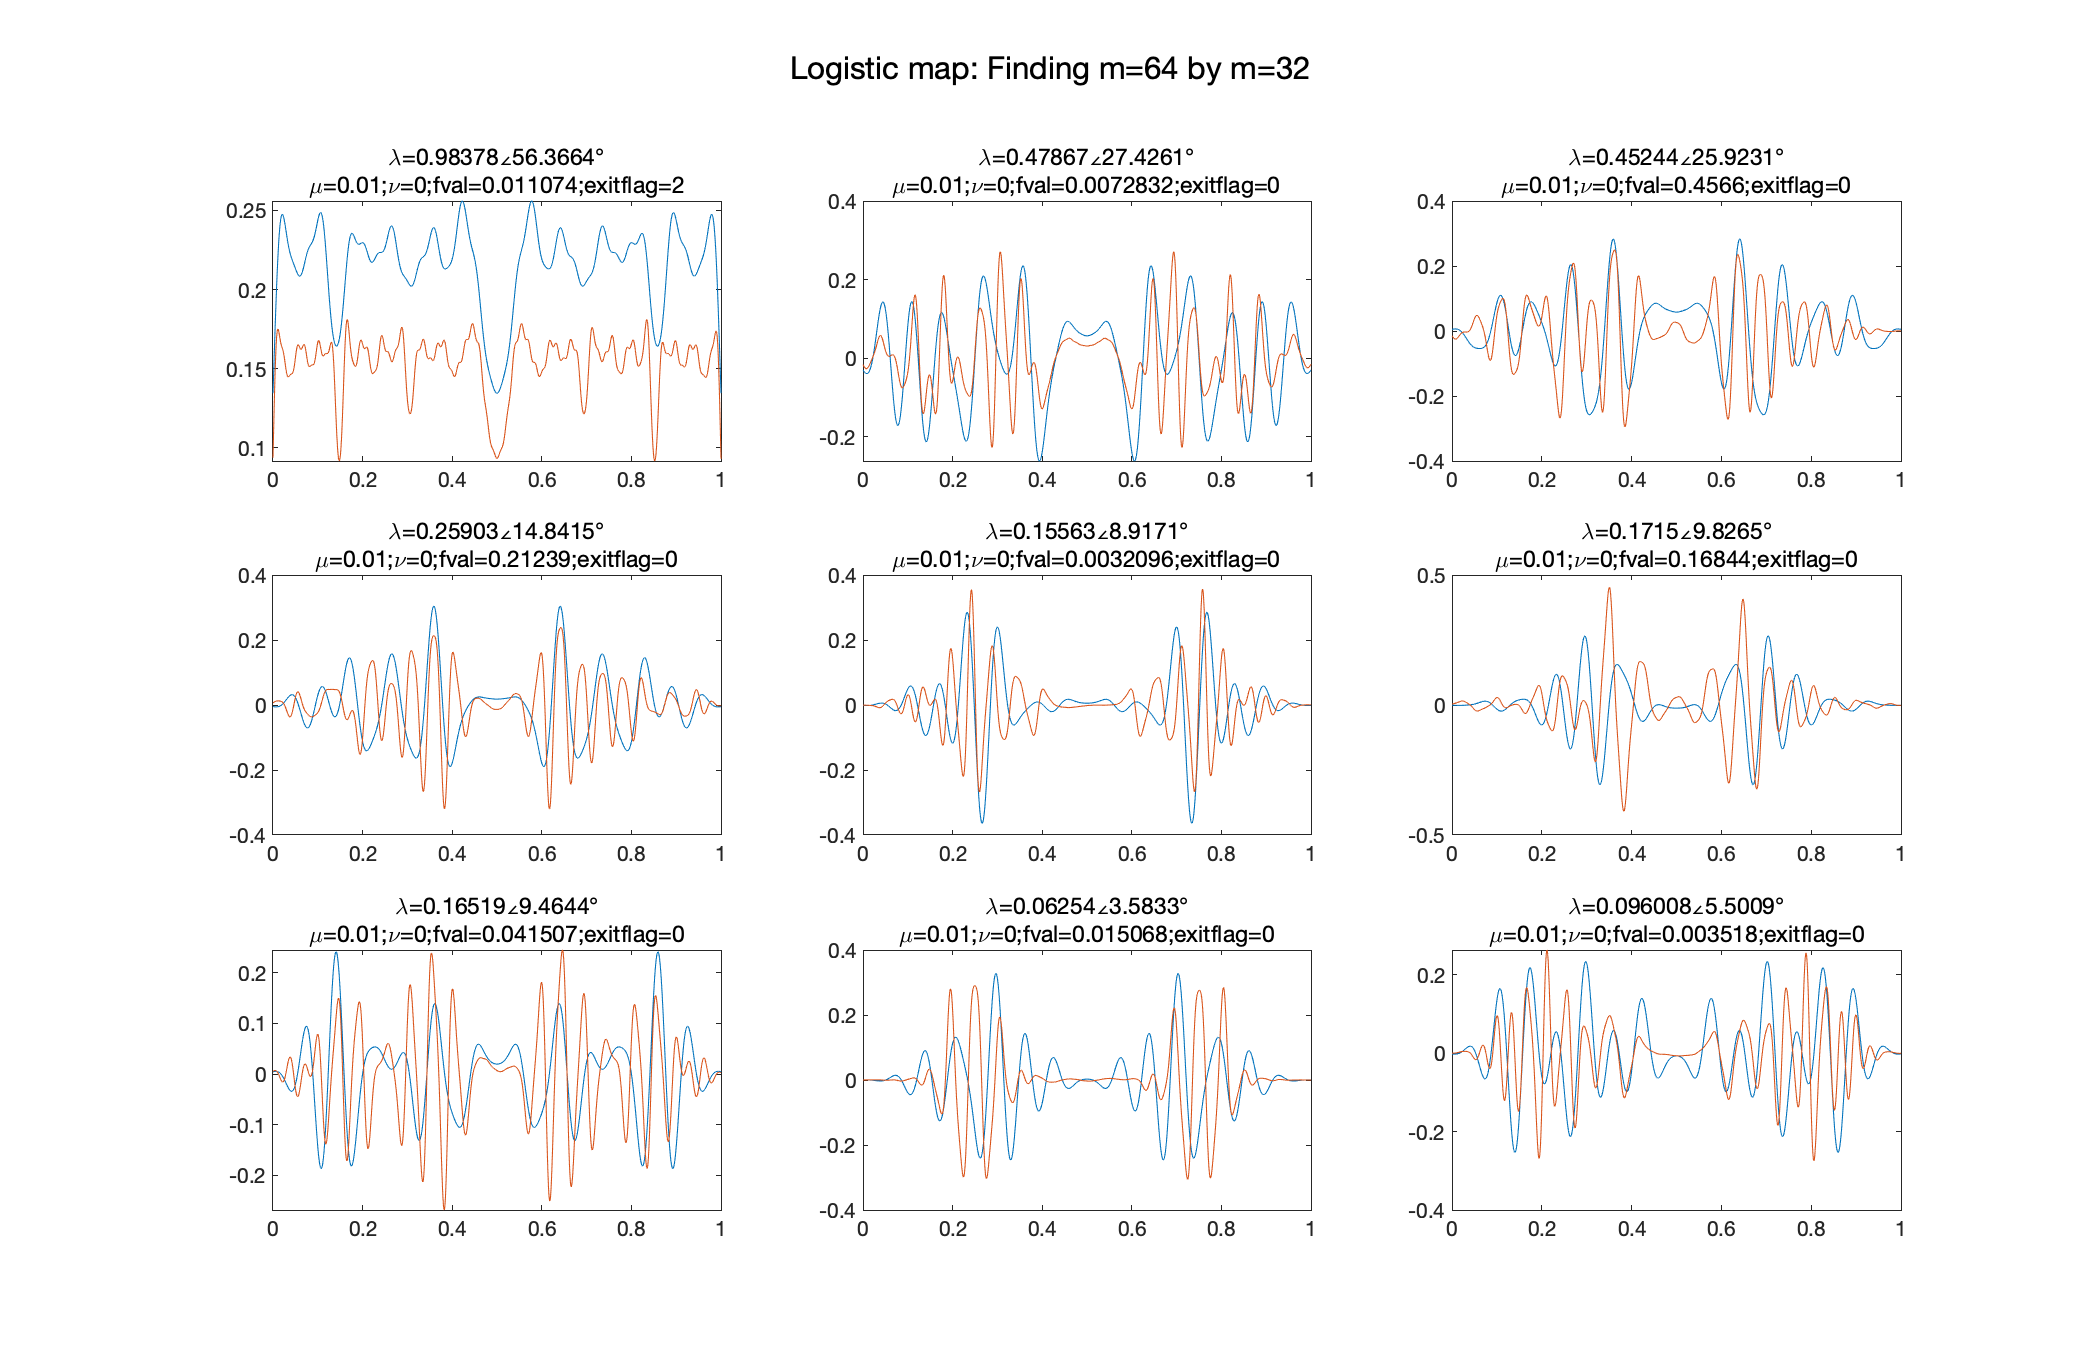
\includegraphics[scale=0.2]{logistic/accurate/Logistic_findeigen_m32m64}}
    \\
  \caption[Logistic映射本征函数不同基函数数量之间的对应关系]{Logistic映射本征函数不同基函数数量之间的对应关系($n=1000$):根据较小基函数数量的本征函数(蓝色)寻找满足条件的较大基函数数量的本征函数(红色)}\label{fig:Logistic_findeigen_m8m16}
\end{figure}

在图\ref{fig:Logistic_findeigen_m8m16}(c)第四个小图中,随着基函数数量扩大一倍,本征函数的极值点的数量也增加了一倍左右,且红色本征值的极值点并未丢失蓝色本征值的极值点,且红色本征值的极值点较蓝色本征值点增加了一些点,通过数据上的验证,我们发现这些多出来的极值点恰好处于某一层次下的Logistic的边界点。这说明了随着基函数数量的增加,本征函数描述边界点的层次有所增加。

这个结论得到了与帐篷映射一致的结论:Koopman算符的本征函数的极值点反映了Logistic映射的边界点,且随着函数格点数量的增加,我们对边界点层次的刻画也更为精细。这为我们寻找不同层次的边界点提供了一种方法:我们可以通过增加本征函数的数量来不断精确我们对边界点的划分,同时可辅以迭代关系来确定边界点的层次。图\ref{fig:Logistic_auto_level_n1000_m4}反映了在不同基函数下通过本征函数极值点及迭代关系确定的边界点的层次。

\begin{figure}[!]
  \centering
  \subfloat[m=4]{
    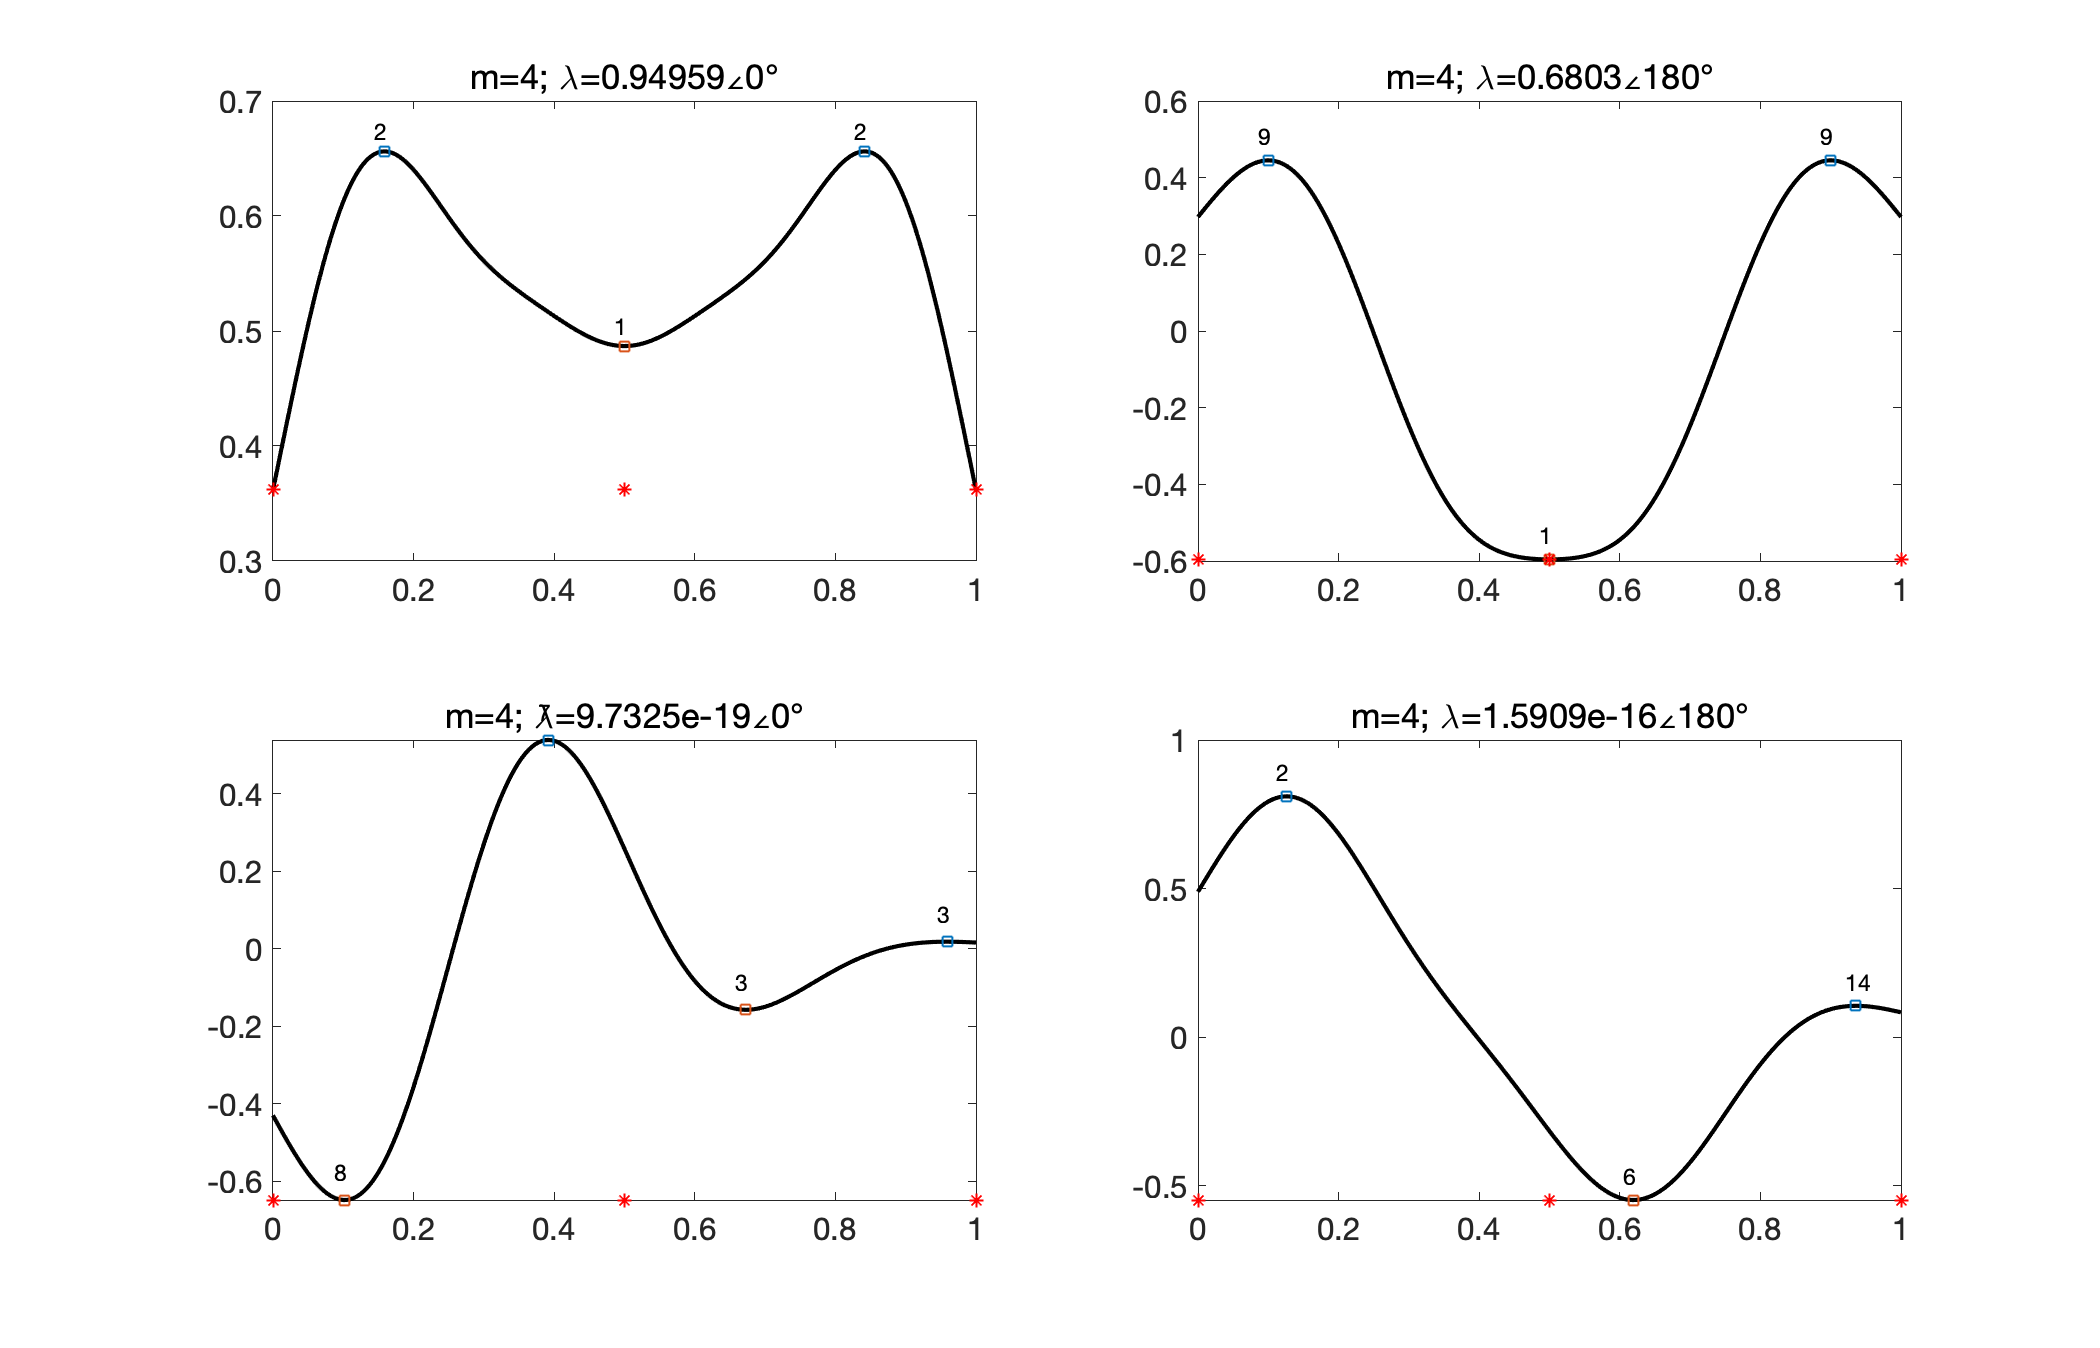
\includegraphics[scale=0.2]{logistic/accurate/Logistic_auto_level_n1000_m4}}
  \subfloat[m=5]{
    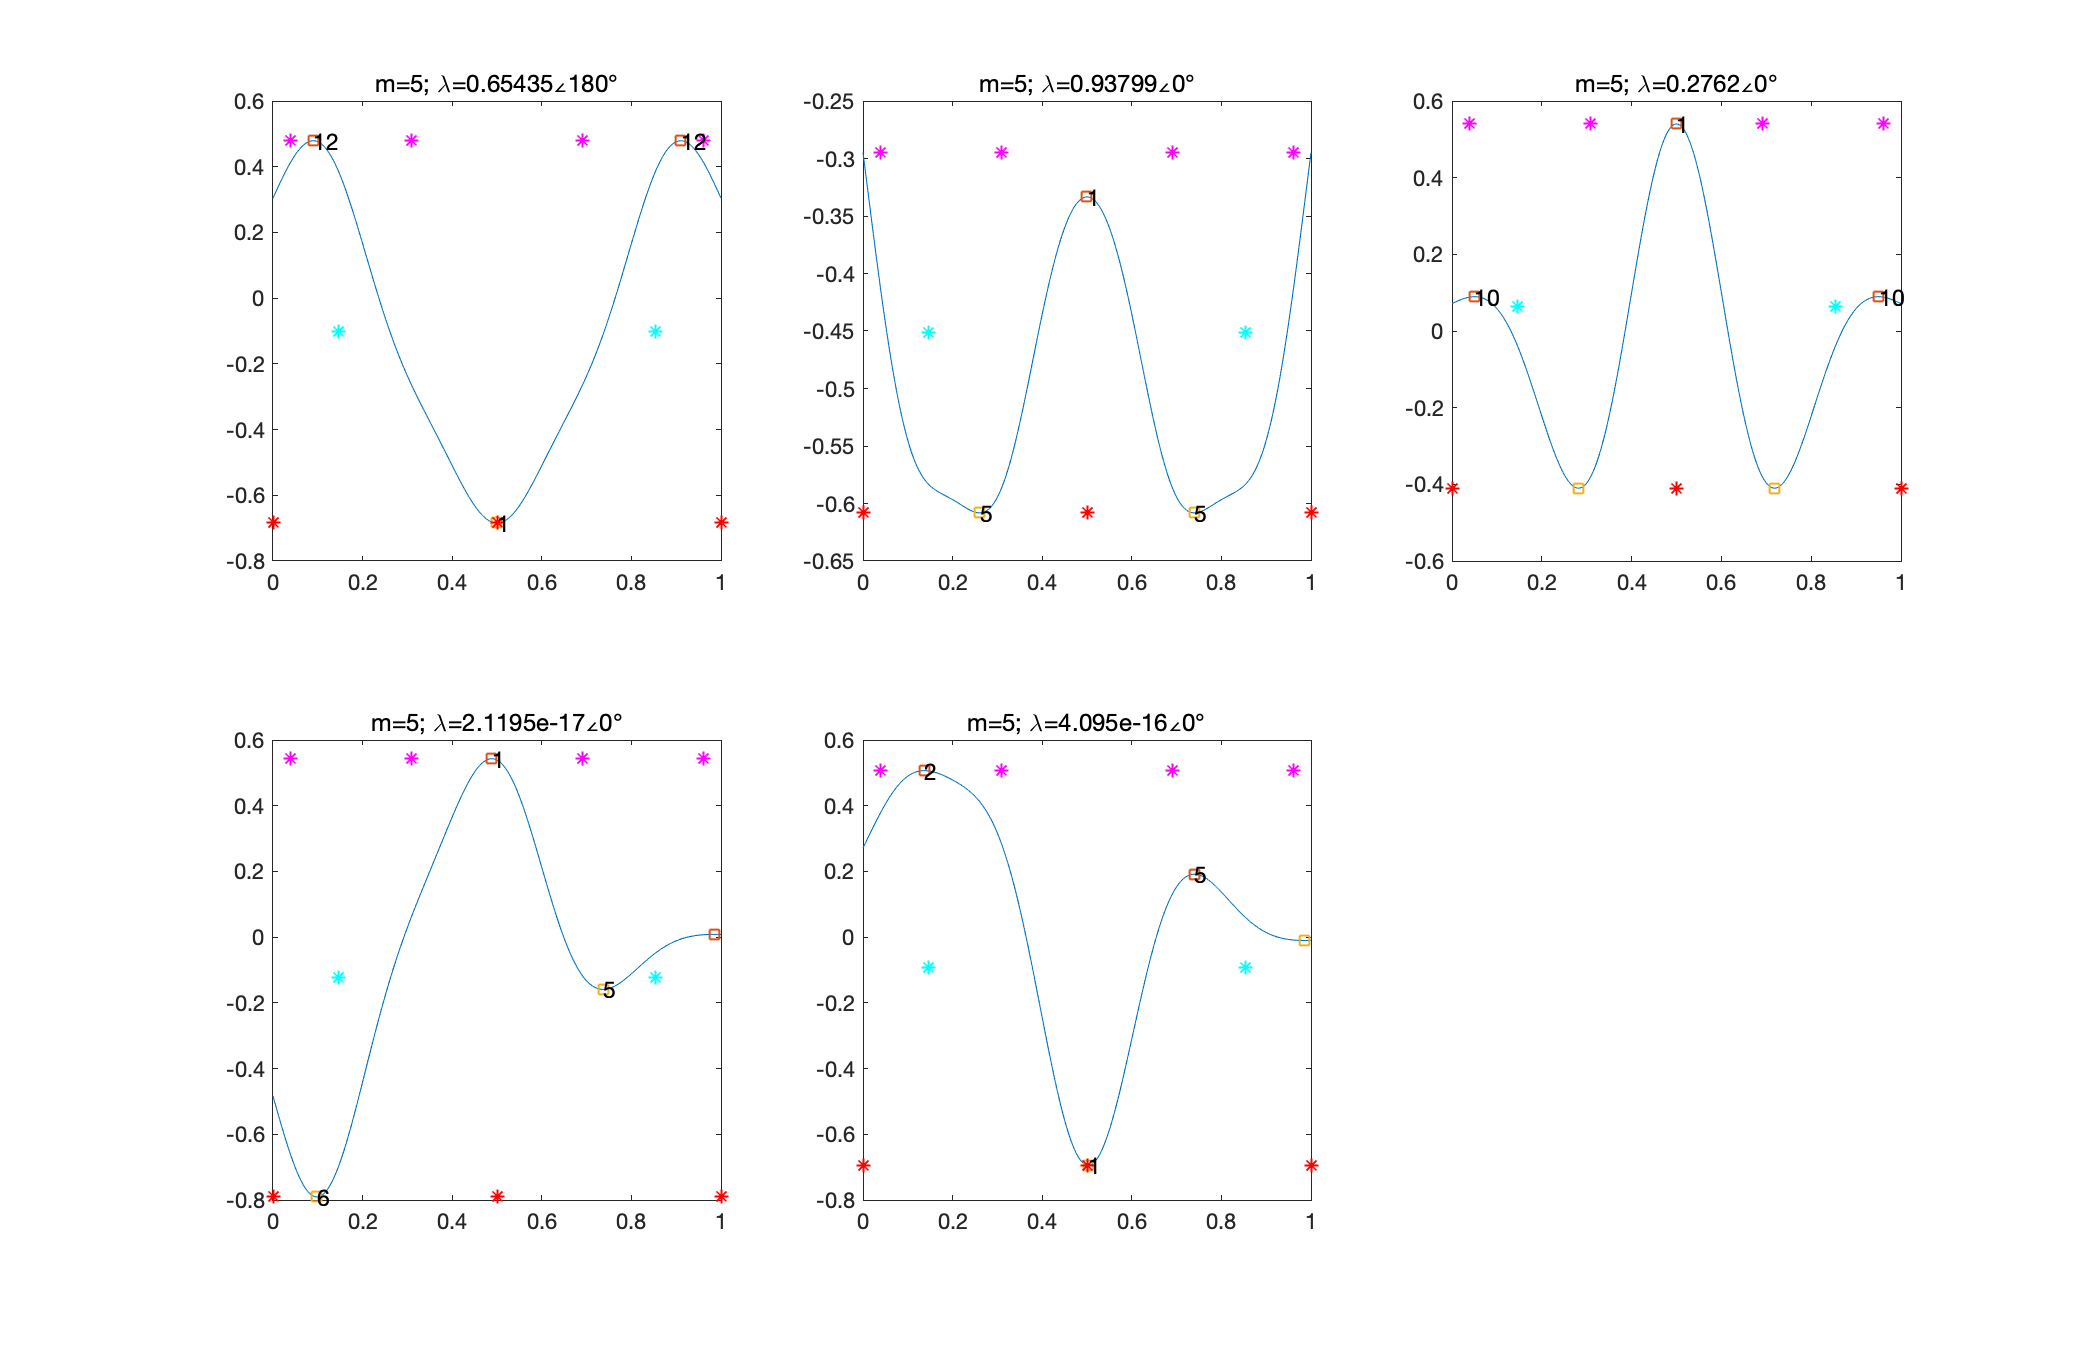
\includegraphics[scale=0.2]{logistic/accurate/Logistic_auto_level_n1000_m5}}
    \\
  \subfloat[m=8]{
    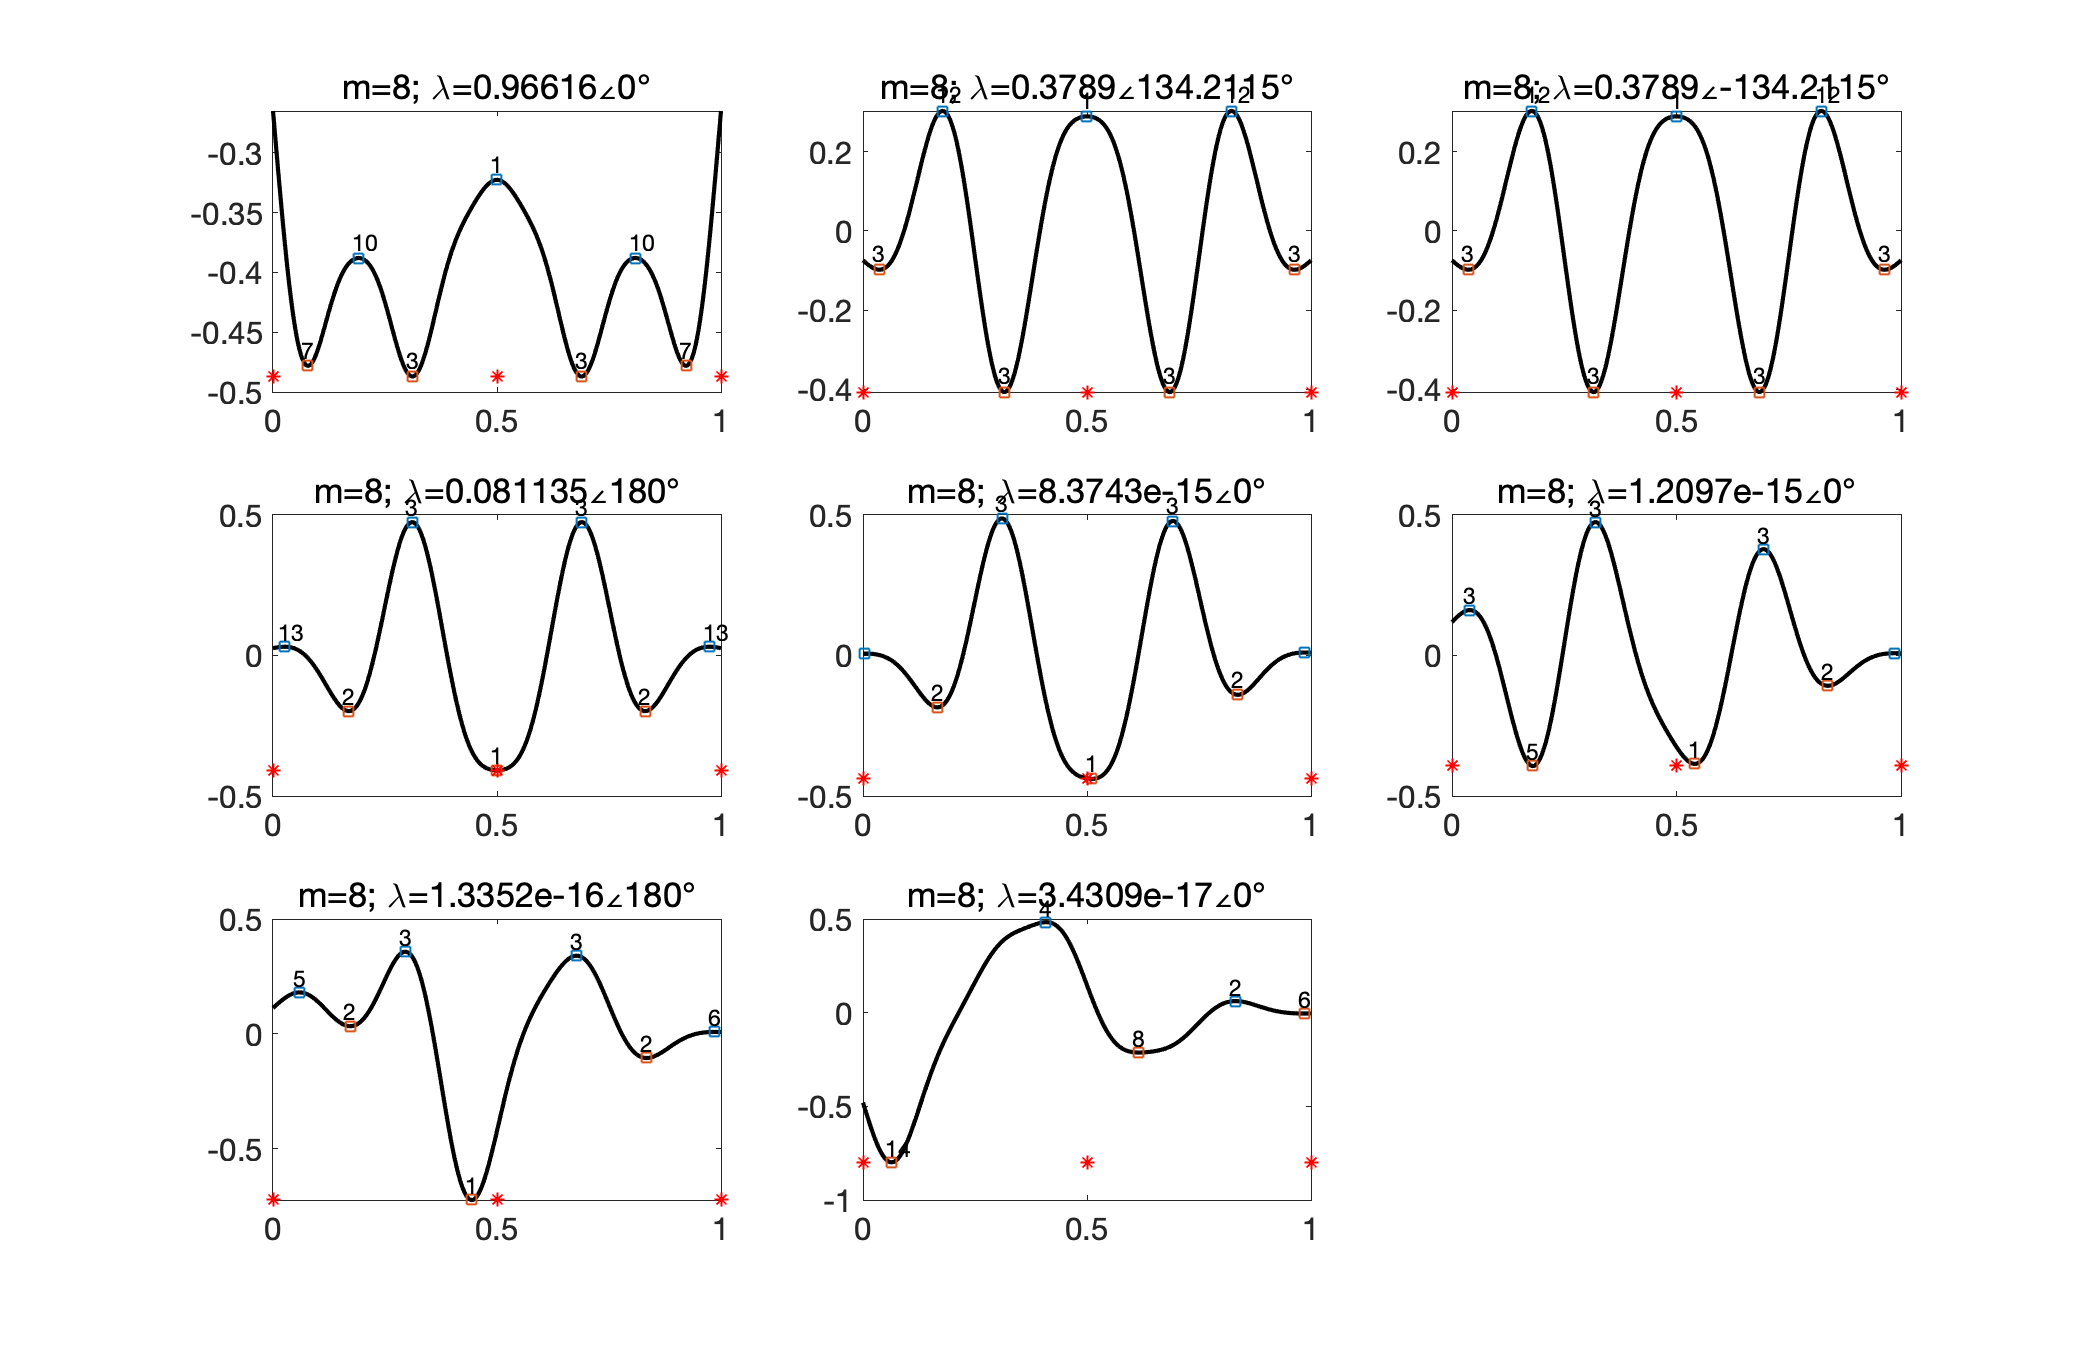
\includegraphics[scale=0.2]{logistic/accurate/Logistic_auto_level_n1000_m8}}
  \subfloat[m=10]{
    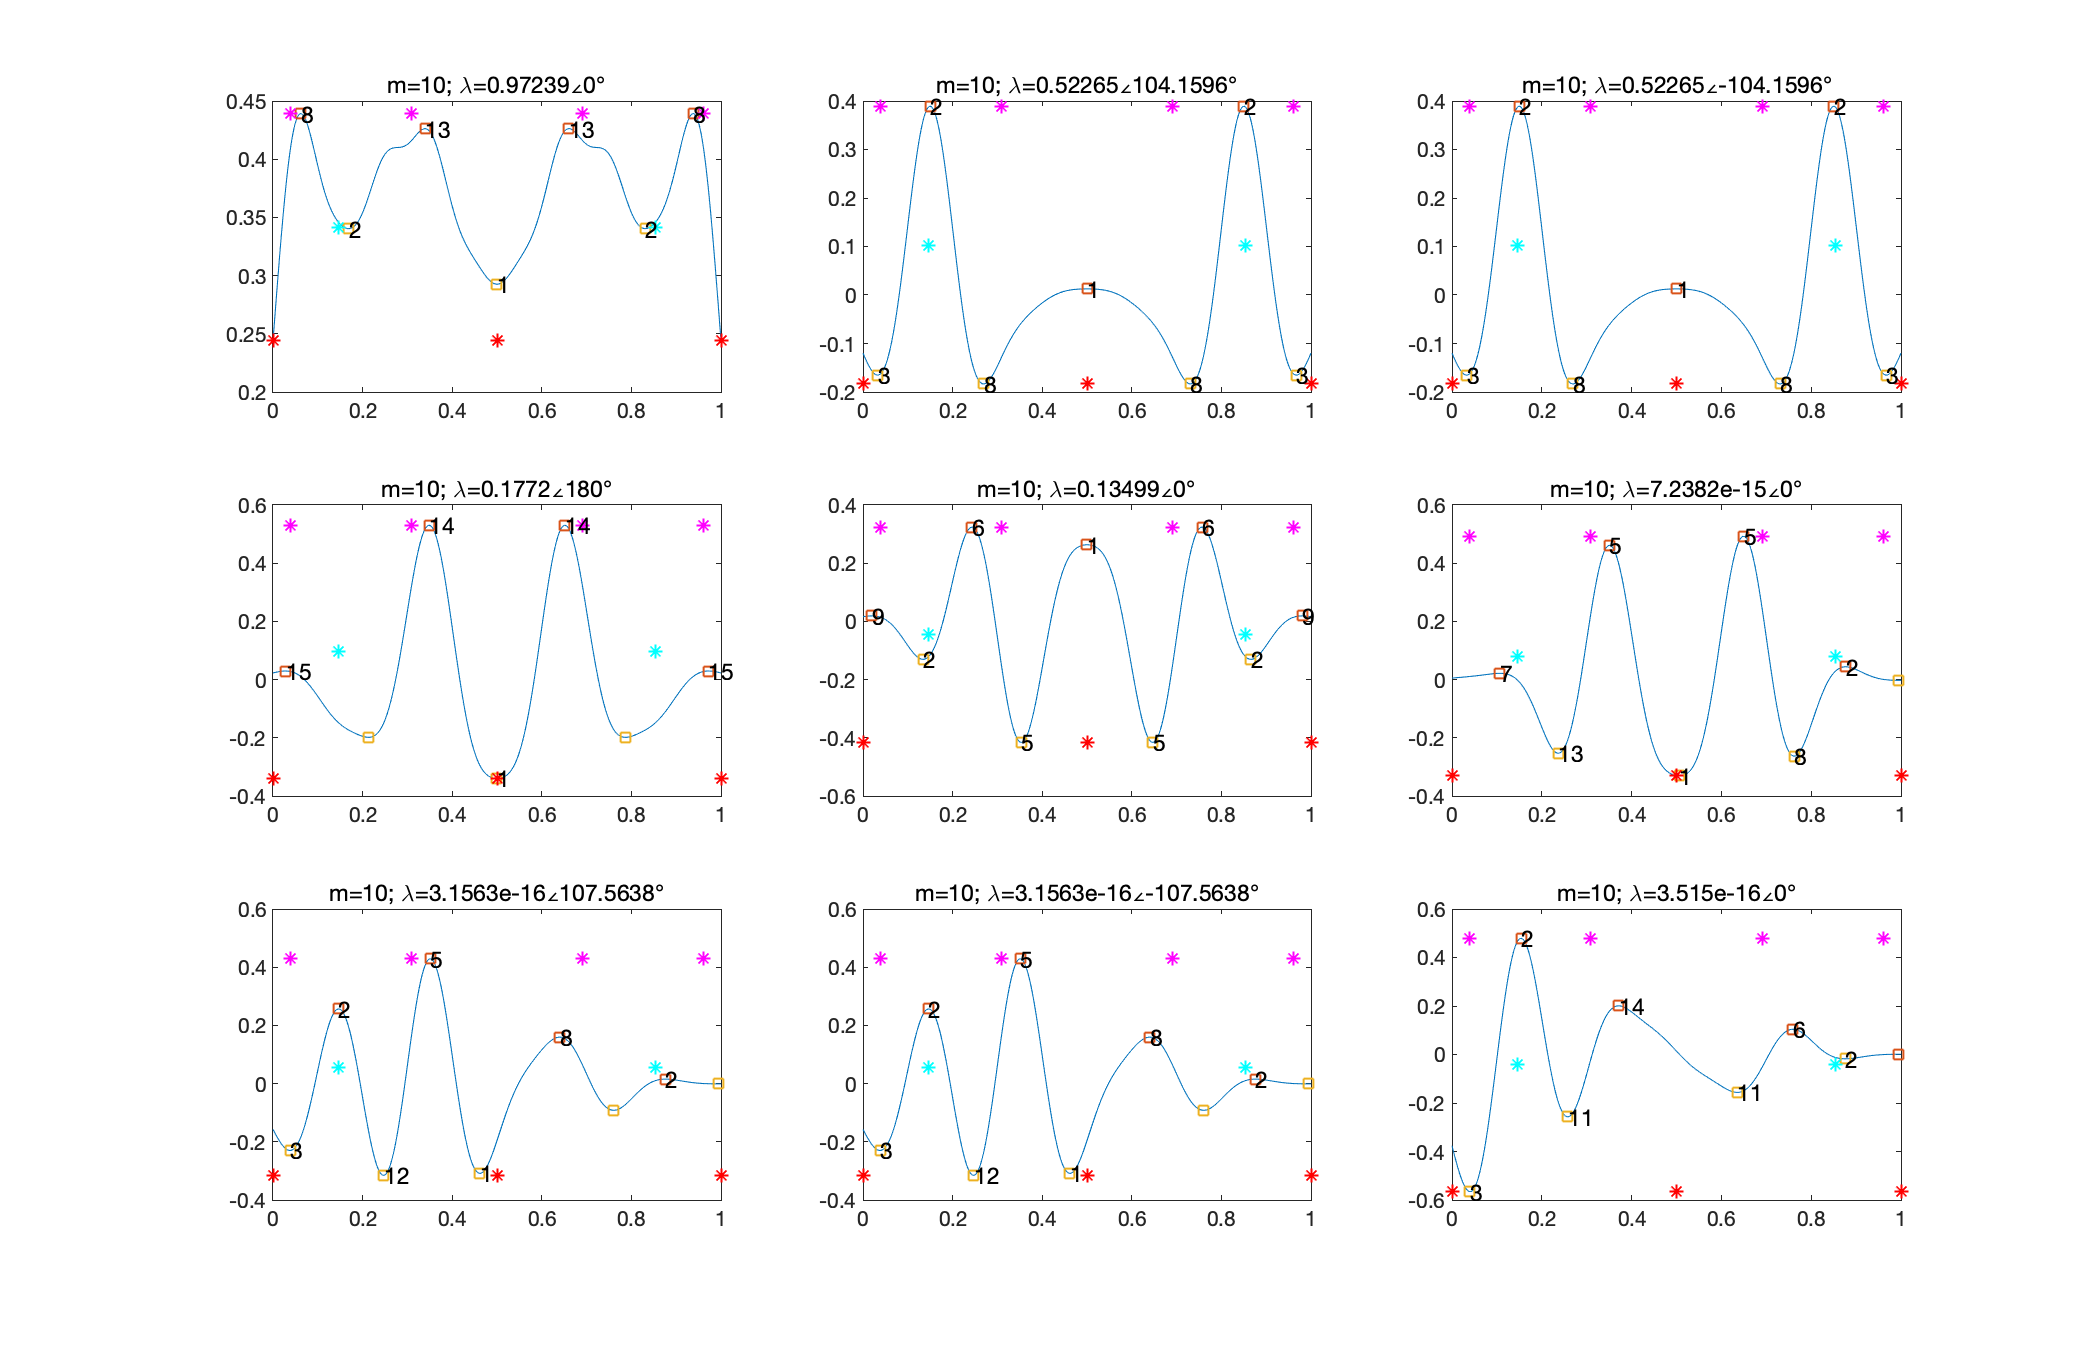
\includegraphics[scale=0.2]{logistic/accurate/Logistic_auto_level_n1000_m10}}
    \\
  \subfloat[m=15]{
    \includegraphics[scale=0.2]{logistic/accurate/Logistic_auto_level_n1000_m15}}
  \subfloat[m=20]{
    \includegraphics[scale=0.2]{logistic/accurate/Logistic_auto_level_n1000_m20}}
    \\
  \caption[Logistic映射本征函数确定边界点层次]{Logistic映射本征函数确定边界点层次($n=1000,noise=0$):红色与青色的点表示Logistic的边界点,空心方块表示本征函数的极值点,且若满足迭代关系则将其边界点的层次标注在极值点附近}\label{fig:Logistic_auto_level_n1000_m4}
\end{figure}
在图\ref{fig:Logistic_auto_level_n1000_m4}中,我们计算了处于层次为15以内的边界点:我们可以发现,很多本征函数的极值点,我们都可以通过迭代关系确定其层次,并识别大部分极值点。我们可以通过Koopman算符确定动力学系统的边界点,且可以通过增加函数格点数量来精确的寻找重要的边界点,而其他层次的边界点也可以通过迭代关系来确定。这个结论与帐篷映射中的结论一致。

%\subsection{小结}


